\documentclass[headings=small,a4paper, 12pt]{scrreprt}

%Schriftart
\usepackage[utf8]{inputenc}
\usepackage[T1]{fontenc}
\usepackage[ngerman]{babel}
%Times New Roman (CZG-Vorgabe: Times New Roman oder Arial, 12 pt)
\usepackage{newtxtext}
\usepackage{romannum} %römische Ziffern in Code: \Romannum{1} (groß) \romannum{1} klein
\usepackage{tabularx}
\usepackage{booktabs}
%schriftgröße der Überschriften
\setkomafont{chapter}{\Large}
\setkomafont{section}{\large}
\setkomafont{subsection}{\normalsize}

%zeilenabstand der itemizes
\usepackage{enumitem}
\setlist[itemize]{itemsep=0pt, parsep=0pt, topsep=0pt, partopsep=0pt}

%beginn fußnoten mit leerzeichen
\deffootnote{1em}{1em}{\makebox[1em][r]{\thefootnotemark\ }}

%normale Fußnoten mit Punkt schließen lassen, wenn noch kein '.', '!', '?' vorhanden
\let\orgfootnote\footnote
\newcommand\myautodot{%
  \ifthenelse{\the\spacefactor>\sfcode`,}{}{.}%
}
\renewcommand\footnote[2][\empty]{%
  \ifx#1\empty%
    \orgfootnote{#2\myautodot}%
  \else%
    \orgfootnote[#1]{#2\myautodot}%
  \fi%
}

%Absätze werden über parskip geregelt. Die Werte sind parskip=true/false/half
%(muss vor geometry stehen, sonst werden die Seitenränder überschrieben)
\KOMAoptions{parskip=half}
%Abbildungs- und Tabellenverzeichnis im Inhaltsverzeichnis aufführen
\KOMAoptions{listof=totoc}
%keine Punkte hinter Gliederungs-/Tabellennummern (auch im Anhang: "Tabelle A.1:")
\KOMAoptions{numbers=noenddot}
%Inhaltsverzeichnis nur bis zur nummerierten Ebene 3 (x.x.x)
\setcounter{tocdepth}{2}

%anpassung seitenränder (CZG: oben, links, rechts 2,5 cm; unten 2,0 cm)
\usepackage[
    left=25mm,   % linker Rand
    right=25mm,  % rechter Rand
    top=25mm,    % oberer Rand
    bottom=20mm, % unterer Rand (bis zum Text)
    footskip=8mm % Seitenzahl ca. 1,2 cm über der Blattkante (wie Fußzeile in Word)
]{geometry}

%Festlegen des Seitenlayouts
\usepackage[onehalfspacing]{setspace} %Zeilenabstand
%alternativ \linespread{1.5}
%Kein BCOR/DIV mehr: KOMA würde damit den Satzspiegel neu berechnen und die
%geometry-Ränder überschreiben.

%Seitenzahlen in der Fußzeile zentriert, keine Kopfzeile
\usepackage[automark]{scrlayer-scrpage}
\clearpairofpagestyles
\cfoot*{\pagemark}
\pagestyle{scrheadings}

%Fußnoten fortlaufend über die ganze Arbeit nummerieren (nicht pro Kapitel)
\counterwithout{footnote}{chapter}

%Name der Verfasserin / des Verfassers in kleinerer Schrift unter der Überschrift
\newcommand{\autor}[1]{\par\noindent{\small\textit{#1}}\par}

%Abstand vor Kapitelbeginn
\RedeclareSectionCommand[
  beforeskip=0pt,
  afterindent=false
]{chapter}

%Schriftart der Überschriften serif in bold
\addtokomafont{disposition}{\rmfamily}
%Schriftart der Überschriften in serif ohne bold
%\setkomafont{disposition}{\normalfont}

%Für das Einfügen eines Glossars: siehe https://en.wikibooks.org/wiki/LaTeX/Glossary

%stützt die Schnittstelle von float und listings zu tocbasic (genutzt von KOMA-script)
\usepackage{scrhack}

%Zum Auskommentieren von größeren Blöcken
\usepackage{comment}
%Als Platzhalter
\usepackage{lipsum}
%Einfachere Verwendung von Anführungszeichen
\newcommand{\qt}[1]{\glqq#1\grqq{}}
%Angabe von Bildquellen
\newcommand{\quelle}[1]{\\\vspace{.1cm}{Quelle: #1}}
%Angabe von Tabellenquellen (unter der Tabelle, Tabellenüberschrift steht oben)
\newcommand{\tabquelle}[1]{\par\vspace{.1cm}{Quelle: #1}}

%Bilder
\usepackage{graphicx}
\usepackage{float}
\graphicspath{{./abbildungen/}}
\usepackage[export]{adjustbox}
\usepackage{array}


%Einfügen von Unformatiertem typewriter Text
\usepackage{verbatim}
%über mehrere Zeilen mit \begin{Verbatim}[breaklines=true]\end{Verbatim}
\usepackage{fancyvrb}


%Alles was das Formelherz begehrt
\usepackage{amstext} 
\usepackage{amsmath}
%newtxmath (Times-Mathematik) enthält die amssymb-Symbole und muss nach amsmath geladen werden
\usepackage{newtxmath}

%Für die Literaturverzeichnisse
\usepackage{csquotes}

%Für Hauptname der Quelle in anderer Schriftart nehme man 'iso-authoryear'. (nutzt dreprecated Feld)




%Literaturverzeichnis exakt nach ISO 690-3
%Eine Alternative Erstellung von Literaturverzeichnissen über natbib (letzte Version von 2010)
%WICHTIG: bei einem Wechsel müssen alle Temporären Dateien von LaTex gelöscht werden!
%\usepackage{natbib}
%\usepackage{multibib} %Unterteilung in Internet- und Printmedien
%\newcites{online}{Internetquellenverzeichnis} 
%Statt \cite{} muss für Internetquellen nun \citeonline{} verwendet werden!



%Anklickbare Links und \url{}
\usepackage{hyperref}
%Zeilenumbrüche in URLs, standard url Paket wird von hyperref geladen, Befehl \url{} bleibt gleich
\usepackage{microtype}[final]
\urlstyle{same}

%glossar
\usepackage[acronym,hyperfirst=true,toc=true]{glossaries}
%\hypersetup{pageanchor=true}
\makeglossaries

%https://de.overleaf.com/learn/latex/Glossaries infos über Erstellung glossareintraäge und aufrufe dieser
%WICHTIG! wenn Änderungen an den Glossareinträgen vorgenommen werden,im Terminal hintereinander das hier iengeben:
%erstmal .glo datei lsöchen, dann:
%
%makeglossaries Seminarfacharbeit
%pdflatex Seminarfacharbeit.tex
%nur dann funktioniert das Glossar auch in der PDF-Datei
%
%CZG-Vorgaben: alphabetisch (wird automatisch nach "name" bzw. "sort" sortiert),
%jede Erklärung 1-2 Sätze. Es erscheinen nur Einträge, die im Text mit \gls{...}
%verwendet werden. Bei kleingeschriebenen Namen "sort" angeben, sonst landen sie am Ende.
\begin{comment}
    zum kopieren:
    \newglossaryentry{}
    {}
\end{comment}

\newglossaryentry{abtastrate}{
    name={Abtastrate},
    first={\textit{Abtastrate}},
    description={Anzahl der Messwerte, die pro Sekunde und Kanal aufgezeichnet werden. Sie wird in Hertz (Hz) angegeben}
}

\newglossaryentry{alphapower}{
    name={Alpha-Power},
    first={\textit{Alpha-Power}},
    description={Leistung des EEG-Signals im Alpha-Band (8--12 Hz), also ein Maß dafür, wie stark die Alpha-Aktivität ausgeprägt ist. Sie wird aus der spektralen Leistungsdichte berechnet und in \textmu V$^2$/Hz angegeben}
}

\newglossaryentry{analog-digital-converter}{
    name={Analog-Digital-Converter},
    first={\textit{Analog-Digital-Converter}},
    description={Auf Deutsch Analog-Digital-Wandler: elektronisches Bauteil, das analoge Signale in einen digitalen Datenstrom umwandelt, der dann weiterverarbeitet oder gespeichert werden kann}
}

\newglossaryentry{baseline_erp}{
    name={Basislinie (in Bezug auf ERPs)},
    first={\textit{Basislinie}},
    description={Auch \textit{Baseline}: Zeitraum direkt vor dem Stimulus, dessen mittlere Spannung als Nullpunkt dient. Bei der Basislinienkorrektur wird dieser Mittelwert von der gesamten Epoche abgezogen}
}

\newglossaryentry{baseline_alpha}{
    name={Basislinie (in Bezug auf Frequenzbänder)},
    first={\textit{Basislinie}},
    description={Auch \textit{Baseline}: Normalwert der Leistung in den Frequenzbändern, der nicht durch Reize oder Aufgaben beeinflusst ist}
}

\newglossaryentry{bandpass}{
    name={Bandpassfilter},
    plural={Bandpassfilter},
    firstplural={\textit{Bandpassfilter}},
    first={\textit{Bandpassfilter}},
    description={Filter, der nur Signale innerhalb eines bestimmten Frequenzbereichs durchlässt}
}

\newglossaryentry{berger-effekt}{
    name={Berger-Effekt},
    first={\textit{Berger-Effekt}},
    description={Blockade der Alpha-Wellen im EEG, die auftritt, wenn eine wache und entspannte Person die Augen öffnet; die Alpha-Wellen werden dann durch Beta-Wellen ersetzt. Beim Schließen der Augen kehrt der Alpha-Rhythmus zurück}
}

\newglossaryentry{brain-computer-interface}{
    name={Brain-Computer-Interface},
    first={\textit{Brain-Computer-Interface}},
    description={Brain-Computer-Interfaces, auf Deutsch Gehirn-Computer-Schnittstellen, sind Systeme, die es ermöglichen, Informationen direkt aus dem Gehirn zu extrahieren und in Befehle für externe Geräte umzuwandeln}
}

\newglossaryentry{brainflow}{
    name={BrainFlow},
    first={\textit{BrainFlow}},
    description={Frei verfügbare Software-Bibliothek, mit der die Daten verschiedener EEG-Geräte, unter anderem von OpenBCI, aufgezeichnet und verarbeitet werden können}
}

\newglossaryentry{claude-code}{
    name={Claude Code},
    description={KI-Assistent des Unternehmens Anthropic, der Programmcode schreiben und ausführen sowie Daten direkt untersuchen kann}
}

\newglossaryentry{cutoff}{
    name={Cut-off-Frequenz},
    first={\textit{Cut-off-Frequenz}},
    description={Grenzfrequenz, ab der ein Filter Signale durchlässt oder unterdrückt}
}

\newglossaryentry{elektrodencluster}{
    name={Elektroden-Cluster},
    plural={Elektroden-Clustern},
    first={\textit{Elektroden-Cluster}},
    firstplural={\textit{Elektroden-Clustern}},
    description={Gruppe benachbarter Elektroden, die gemeinsam ausgewertet werden, um die Aktivität einer bestimmten Hirnregion zu erfassen. Die Cluster werden nach den Hirnregionen benannt, über denen sie liegen. Die Elektroden, die den Okzipital-Cluster bilden, sind O1, O2, P7 und P8}
}

\newglossaryentry{elektrolyt}{
    name={Elektrolyt},
    first={\textit{Elektrolyt}},
    description={Ein Elektrolyt ist eine Substanz, die elektrische Ladungen leiten kann, wenn sie als Lösung oder im geschmolzenen Zustand vorliegt}
}

\newglossaryentry{epikrImpulse}{
    name={Epikritische Impulse},
    first={\textit{Epikritische Impulse}},
    description={Feine Sinnesreize wie Berührung oder Druck, die präzise wahrgenommen und genau lokalisiert werden können}
}

\newglossaryentry{epoche}{
    name={Epoche},
    plural={Epochen},
    first={\textit{Epoche}},
    firstplural={\textit{Epochen}},
    description={Kurzer Ausschnitt der fortlaufenden EEG-Aufzeichnung um ein Ereignis herum, zum Beispiel von kurz vor bis knapp eine Sekunde nach dem Erscheinen eines Stimulus}
}

\newglossaryentry{eventmarker}{
    name={Ereignismarker},
    plural={Ereignismarkern},
    first={\textit{Ereignismarker}},
    firstplural={\textit{Ereignismarkern}},
    description={Zeitliche Markierung im EEG-Signal zur Kennzeichnung eines Stimulus oder Ereignisses}
}

\newglossaryentry{grand-average}{
    name={Grand Average},
    first={\textit{Grand Average}},
    description={Gruppenmittelung: Mittelwert der ERP-Verläufe über mehrere Versuchspersonen, gebildet aus den zuvor für jede Person einzeln gemittelten Verläufen}
}

\newglossaryentry{mne}{
    name={MNE},
    first={\textit{MNE}},
    description={Frei verfügbare Python-Bibliothek (MNE-Python) zur Verarbeitung und Auswertung von EEG-Daten}
}

\newglossaryentry{messwiederholung}{
    name={Messwiederholung},
    first={\textit{Messwiederholung}},
    description={Versuchsaufbau, bei dem dieselben Personen alle Bedingungen durchlaufen. Dadurch können Unterschiede zwischen den Personen herausgerechnet und Effekte der Bedingungen zuverlässiger erkannt werden}
}

\newglossaryentry{neurofeedback}{
    name={Neurofeedback},
    first={\textit{Neurofeedback}},
    description={Training, bei dem die eigene Hirnaktivität in Echtzeit zurückgemeldet wird (z.\,B. als Bild oder Ton), sodass man lernt, sie gezielt zu beeinflussen}
}

\newglossaryentry{neuroprothese}{
    name={Neuroprothese},
    plural={Neuroprothesen},
    first={\textit{Neuroprothese}},
    firstplural={\textit{Neuroprothesen}},
    description={Technisches Hilfsmittel, das ausgefallene Funktionen des Nervensystems ersetzt oder unterstützt, z.\,B. durch elektrische Stimulation gelähmter Muskeln}
}

\newglossaryentry{no-switzerland-principle}{
    name={No-Switzerland-Prinzip},
    first={\textit{No-Switzerland-Prinzip}},
    description={Bezeichnung dafür, dass es am Körper keinen elektrisch völlig neutralen Ort für eine Referenzelektrode gibt. Jede Wahl der Referenz beeinflusst daher die gemessenen Spannungen}
}

\newglossaryentry{notch}{
    name={Notch-Filter},
    first={\textit{Notch-Filter}},
    description={Filter, der gezielt eine bestimmte Frequenz (z.\,B. 50 Hz Netzrauschen) unterdrückt}
}

\newglossaryentry{oligo}{
    name={Oligodendrozyten},
    first={\textit{Oligodendrozyten}},
    description={Spezialisierte Zellen im zentralen Nervensystem, die Nervenfasern mit einer schützenden Myelinschicht umhüllen}
}

\newglossaryentry{openbci-board}{
    name={OpenBCI-Board},
    first={\textit{OpenBCI-Board}},
    description={Platine von OpenBCI, die die Signale der Elektroden verstärkt, digitalisiert und drahtlos an einen Computer sendet}
}

\newglossaryentry{p300}{
    name={P300},
    first={\textit{P300}},
    description={ERP-Komponente, die etwa 300 ms nach einem seltenen oder bedeutsamen Stimulus auftritt}
}

\newglossaryentry{periphere Nervensystem}{
    name={periphere Nervensystem},
    sort={Periphere Nervensystem},
    first={\textit{periphere Nervensystem}},
    description={Das periphere Nervensystem umfasst alle Nerven außerhalb des zentralen Nervensystems (Gehirn und Rückenmark) und verbindet diese mit den Organen, Muskeln und der Haut}
}

\newglossaryentry{ProtoImpulse}{
    name={Protopathische Impulse},
    first={\textit{Protopathische Impulse}},
    description={Grobe Sinnesreize wie Schmerz oder Temperatur, die weniger genau unterschieden werden können}
}

\newglossaryentry{rückenmark}{
    name={Rückenmark},
    first={\textit{Rückenmark}},
    description={Teil des zentralen Nervensystems, der im Wirbelkanal liegt und als Hauptleitung für Nervenimpulse zwischen Gehirn und Körper dient}
}

\newglossaryentry{snrgl}{
    name={Signal-Rausch-Verhältnis},
    first={\textit{Signal-Rausch-Verhältnis}},
    description={Verhältnis der Stärke des gesuchten Signals zur Stärke der Störungen (des Rauschens). Je größer der Wert, desto deutlicher hebt sich das Signal vom Rauschen ab}
}

\newglossaryentry{silber-silberchlorid-elektrode}{
    name={Silber-Silberchlorid-Elektrode},
    plural={Silber-Silberchlorid-Elektroden},
    first={\textit{Silber-Silberchlorid-Elektrode}},
    firstplural={\textit{Silber-Silberchlorid-Elektroden}},
    description={Häufig in der Elektroenzephalographie verwendete Elektrode aus einem Silberdraht, der mit einer Schicht aus Silberchlorid überzogen ist}
}

\newglossaryentry{psdgl}{
    name={Spektrale Leistungsdichte},
    first={\textit{spektrale Leistungsdichte}},
    description={Beschreibt, wie sich die Leistung eines EEG-Signals auf die verschiedenen Frequenzen verteilt. Dadurch werden Rhythmen wie Delta-, Theta-, Alpha- und Beta-Wellen sichtbar}
}

\newglossaryentry{spline}{
    name={Sphärische Spline-Interpolation},
    first={\textit{sphärischer Spline-Interpolation}},
    description={Mathematisches Verfahren, das die Spannung an einer fehlenden Elektrode aus den Spannungen der übrigen Elektroden auf einer kugelförmigen Kopfoberfläche schätzt}
}

\newglossaryentry{standardabweichung}{
    name={Standardabweichung},
    first={\textit{Standardabweichung}},
    description={Maß für die Streuung von Messwerten um ihren Mittelwert. Je größer sie ist, desto stärker weichen die einzelnen Werte voneinander ab}
}

\newglossaryentry{stimulus}{
    name={Stimulus},
    plural={Stimuli},
    first={\textit{Stimulus}},
    firstplural={\textit{Stimuli}},
    description={Ein Stimulus (Mehrzahl Stimuli) ist ein Reiz, der eine bestimmte körperliche oder psychische Reaktion auslöst}
}

\newglossaryentry{trigger}{
    name={Trigger},
    plural={Trigger},
    description={Zahlencode, der während der Messung in die EEG-Aufzeichnung geschrieben wird, um festzuhalten, wann ein Ereignis, z.\,B. das Erscheinen eines Stimulus, stattfindet}
}

\newglossaryentry{varianzanalyse}{
    name={Varianzanalyse},
    first={\textit{Varianzanalyse}},
    description={Statistisches Verfahren, das prüft, ob sich die Mittelwerte mehrerer Bedingungen systematisch unterscheiden. Dazu werden die Unterschiede zwischen den Bedingungen mit den zufälligen Schwankungen innerhalb der Bedingungen verglichen}
}

\newglossaryentry{wernick}{
    name={Wernicke-Sprachzentrum},
    first={\textit{Wernicke-Sprachzentrum}},
    description={Gehirnbereich, der für das Verstehen von gesprochener und geschriebener Sprache zuständig ist}
}

\newglossaryentry{welch}{
    name={Welch-Methode},
    first={\textit{Welch-Methode}},
    description={Verfahren zur Bestimmung der spektralen Leistungsdichte, bei dem das Signal in überlappende Abschnitte geteilt wird, deren Spektren berechnet und anschließend gemittelt werden. Dadurch entsteht eine stabilere Darstellung der Frequenzanteile}
}


\newglossaryentry{elektrodenimpedanz}{
    name={Elektrodenimpedanz},
    first={\textit{Elektrodenimpedanz}},
    description={Elektrischer Widerstand für Wechselströme am Übergang zwischen Elektrode und Kopfhaut. Je höher er ist, desto schwächer und verrauschter wird das gemessene Signal}
}
\newglossaryentry{validierungsstudie}{
    name={Validierungsstudie},
    first={\textit{Validierungsstudie}},
    description={Untersuchung, die prüft, ob ein Messgerät oder Verfahren tatsächlich das misst, was es messen soll, meist durch Vergleich mit einem anerkannten Referenzverfahren}
}
\newglossaryentry{topographie}{
    name={Topographie},
    first={\textit{Topographie}},
    description={Räumliche Verteilung eines EEG-Signals über die Kopfoberfläche, also an welchen Elektroden es wie stark auftritt}
}
\newglossaryentry{posterior}{
    name={posterior}, sort={Posterior},
    first={\textit{posterior}},
    description={Anatomische Lagebezeichnung für hinten liegend, also zum Hinterkopf hin}
}
\newglossaryentry{anterior}{
    name={anterior}, sort={Anterior},
    first={\textit{anterior}},
    description={Anatomische Lagebezeichnung für vorne liegend, also zur Stirn hin}
}
\newglossaryentry{lateral}{
    name={lateral}, sort={Lateral},
    first={\textit{lateral}},
    description={Anatomische Lagebezeichnung für seitlich, also von der Mittellinie des Kopfes weg zur Seite hin}
}
\newglossaryentry{hochpass}{
    name={Hochpassfilter},
    first={\textit{Hochpassfilter}},
    description={Filter, der nur Frequenzen oberhalb einer Grenzfrequenz durchlässt und damit langsame Schwankungen wie Drifts entfernt}
}
\newglossaryentry{tiefpass}{
    name={Tiefpassfilter},
    first={\textit{Tiefpassfilter}},
    description={Filter, der nur Frequenzen unterhalb einer Grenzfrequenz durchlässt und damit schnelle Störungen wie Muskelrauschen entfernt}
}
\newglossaryentry{durchschnittsreferenz}{
    name={Durchschnittsreferenz},
    first={\textit{Durchschnittsreferenz}},
    description={Referenz, bei der der Mittelwert der Spannungen aller Elektroden als Bezugspunkt dient. Dieser Mittelwert wird von jeder Elektrode abgezogen (Re-Referenzierung)}
}
\newglossaryentry{paradigma}{
    name={Paradigma},
    plural={Paradigmen},
    first={\textit{Paradigma}},
    firstplural={\textit{Paradigmen}},
    description={Standardisierter Versuchsablauf aus Aufgabe, Reizen und Messgröße, mit dem ein bekanntes Hirnsignal zuverlässig ausgelöst und gemessen werden kann}
}
\newglossaryentry{spearman}{
    name={Rangkorrelation nach Spearman},
    first={\textit{Rangkorrelation nach Spearman}},
    description={Statistisches Maß ($\rho$) zwischen $-1$ und $1$ dafür, wie stark zwei Rangfolgen übereinstimmen. Ein Wert von 1 bedeutet identische Reihenfolge, 0 keinen Zusammenhang}
}
\newglossaryentry{zufallsniveau}{
    name={Zufallsniveau},
    first={\textit{Zufallsniveau}},
    description={Trefferquote, die man durch bloßes Raten erreichen würde, bei zwei gleich wahrscheinlichen Möglichkeiten also 50\,\%}
}
\newglossaryentry{inferenzstatistik}{
    name={Inferenzstatistik},
    first={\textit{Inferenzstatistik}},
    description={Teilgebiet der Statistik, das mit Tests prüft, ob ein in einer Stichprobe beobachteter Unterschied auf die Gesamtheit übertragbar oder nur zufällig entstanden ist}
}
\newglossaryentry{spektralanalyse}{
    name={Spektralanalyse},
    first={\textit{Spektralanalyse}},
    description={Zerlegung eines Signals in seine einzelnen Frequenzanteile, um zu bestimmen, wie stark jede Frequenz im Signal vertreten ist}
}
\newglossaryentry{smr}{
    name={Sensomotorischer Rhythmus},
    plural={Sensomotorische Rhythmen},
    first={\textit{Sensomotorischer Rhythmus}},
    description={Rhythmus über den motorischen und sensorischen Hirnarealen, z.\,B. der $\mu$-Rhythmus (etwa 8--13\,Hz), der bei Bewegung oder Bewegungsvorstellung schwächer wird}
}
\newglossaryentry{intrakortikal}{
    name={intrakortikal}, sort={Intrakortikal},
    first={\textit{intrakortikal}},
    description={Innerhalb der Großhirnrinde (Cortex) gelegen. Intrakortikale Implantate sind Elektroden, die operativ direkt in das Hirngewebe eingesetzt werden}
}
\newglossaryentry{bias}{
    name={Bias},
    first={\textit{Bias}},
    description={Systematische Verzerrung von Messergebnissen in eine bestimmte Richtung, die nicht zufällig ist und sich daher durch Mittelung nicht beseitigen lässt}
}

\newglossaryentry{zufallsgrenze}{
    name={Zufallsgrenze},
    first={\textit{Zufallsgrenze}},
    description={Trefferquote, die durch bloßes Raten nur mit einer Wahrscheinlichkeit von unter 5\,\% erreicht wird. Sie liegt über dem Zufallsniveau und hängt von der Anzahl der Entscheidungen ab}
}

\newglossaryentry{Comma-Separated Values}{
    name={Comma-Separated Values},
    first={\textit{Comma-Separated Values}},
    description={Ein einfaches Textformat zum Speichern von Tabellendaten, bei dem jede Zeile einem Datensatz entspricht und die einzelnen Werte durch ein Trennzeichen, meist ein Komma, voneinander getrennt sind}
}




%hier kommen die Einträge für das Abkürzungsverzeichnis rein
%so:
%\newacronym{label}{abkürzung}{lang}

\newacronym{csv}{CSV}{Comma-Separated Values}
\newacronym{bdf}{BDF}{BioSemi Data Format}

\newacronym{eeg}{EEG}{Elektroenzephalographie oder Elektroenzephalogramm}

\newacronym{bci}{BCI}{Brain-Computer-Interface}

\newacronym{epsp}{EPSP}{exzitatorisches / erregendes postsynaptisches Potenzial}

\newacronym{ipsp}{IPSP}{inhibitorisches / hemmendes postsynaptisches Potenzial}

\newacronym{adc}{ADC}{Analog-Digital-Converter}

\newacronym{erps}{ERPs}{Mehrzahl von \acrshort{erp}}

\newacronym{erp}{ERP}{Aus dem Englischen \emph{event-related potentials}, \glqq ereignisbezogene Potenziale\grqq, Mehrzahl ERPs}

\newacronym{dc}{DC}{Direct Current}

\newacronym{eog}{EOG}{Elektrookulographie}

\newacronym{cms}{CMS}{Common-Sense}

\newacronym{drl}{DRL}{Driven-Right-Leg}

\newacronym{ica}{ICA}{Independent Component Analysis}

\newacronym{ekp}{EKPs}{ereigniskorrelierte Potenziale}

\newacronym{pt}{pt}{Participant}

%gkleiche abstände zwischen den Absätzen
\newglossarystyle{acrostyle}{%
  \setglossarystyle{long}%
  \setlength{\glsdescwidth}{0.7\textwidth}%
}



%Formatierung und Import Bibliography

\usepackage[affil-it]{authblk}	
%Zitierweise nach CZG: Kurzbeleg in der Fußnote "Vgl. Familienname (Jahr): S. x."
%Quellenverzeichnis: alle Autor:innen (maxbibnames=99); im Kurzbeleg ab 3 Autor:innen
%immer "Erstautor et al." (Anmerkung der Fachlehrerin, abweichend vom CZG-Dokument,
%das bei 3-5 Autor:innen bei der Erstnennung alle Namen vorsieht).
\usepackage[datamodel=datamodel,backend=biber,style=authoryear,autocite=footnote,
  maxbibnames=99,minbibnames=99,maxcitenames=5,mincitenames=1,
  uniquename=false,uniquelist=false,citetracker=true,ibidtracker=constrict,pagetracker=true,
  urldate=short,lasteditdate=long,dateabbrev=false]{biblatex}
\addbibresource{literatur.bib}
\setlength{\bibitemsep}{1.5em}

% slash zwischen namen 
\DeclareDelimFormat{multinamedelim}{\space\slash\space}
\DeclareDelimFormat{finalnamedelim}{\space\slash\space}
%Vor und nach name richtige reinfolge
\DeclareNameAlias{sortname}{family-given}   
\DeclareNameAlias{default}{family-given}    

\DefineBibliographyStrings{ngerman}{
  urlseen = {Abrufdatum},
  andothers = {et\addabbrvspace al\adddot}
}

%URL ohne vorangestelltes "url:"; Abrufdatum als [Abrufdatum TT.MM.JJJJ]
\DeclareFieldFormat{url}{\url{#1}}
\DeclareFieldFormat{pages}{S\adddot\addnbspace#1}
\DeclareFieldFormat{edition}{\ifinteger{#1}{#1\adddot\addspace Aufl\adddot}{#1}}

%Kurzbeleg (\cite): Druckquellen "Familienname (Jahr)", Internetquellen
%"Autor/Institution (Abrufdatum)", Lexika "Lexikon: Stichwort (Abrufdatum)".
%Gibt es von derselben Institution mehrere Seiten mit gleichem Abrufdatum, steht
%zusätzlich das Feld shorttitle hinter dem Namen.
\newbibmacro{czg:abrufdatum}{%
  \printtext[parens]{\mkbibdateshort{urlyear}{urlmonth}{urlday}}}
\newbibmacro{czg:cite}{%
  \ifentrytype{onlinelexikon}
    {\printtext{\thefield{journaltitle}\addcolon\space\thefield{title}}%
     \setunit{\addspace}\usebibmacro{czg:abrufdatum}}
    {\printnames{labelname}%
     \ifboolexpr{test {\ifentrytype{onlinedokument}} and not test {\iffieldundef{urlyear}}}
       {\iffieldundef{shorttitle}{}{\printtext{\addcolon\space\thefield{shorttitle}}}%
        \setunit{\addspace}\usebibmacro{czg:abrufdatum}}
       {\setunit{\addspace}\printtext[parens]{\printlabeldateextra}}}}

%"Ebd." in Fußnoten, wenn direkt davor dieselbe Quelle allein zitiert wurde,
%aber nicht in der ersten Fußnote einer Seite (ibidtracker=constrict, pagetracker)
\newtoggle{czg:ibid}
\DeclareCiteCommand{\cite}
  {\global\togglefalse{czg:ibid}\usebibmacro{prenote}}
  {\usebibmacro{citeindex}%
   \ifboolexpr{test {\iffootnote} and test {\ifciteibid} and not test {\iffirstonpage}}
     {\global\toggletrue{czg:ibid}\printtext{Ebd\adddot}}
     {\usebibmacro{czg:cite}}}
  {\multicitedelim}
  {\iftoggle{czg:ibid}
     {\iffieldundef{postnote}{}{\setunit{\addcomma\space}\printfield{postnote}}}
     {\usebibmacro{postnote}}}
\DeclareDelimFormat{postnotedelim}{\addcolon\space}
\DeclareFieldFormat{postnote}{#1}
\renewcommand*{\multicitedelim}{\addsemicolon\space}

%ab 3 Autor:innen immer "et al." (siehe oben)
%Endet die Autorenliste im Literatureintrag mit "and others" (mehr Autor:innen als
%eingetragen), steht von Anfang an "Erstautor et al."
\AtEveryCitekey{\defcounter{maxnames}{2}%
  \ifandothers{labelname}{\defcounter{maxnames}{1}}{}}

%Datum ohne Leerzeichen: TT.MM.JJJJ
\DefineBibliographyExtras{ngerman}{%
  \protected\def\mkbibdateshort#1#2#3{%
    \iffieldundef{#3}{}{\mkdayzeros{\thefield{#3}}.}%
    \iffieldundef{#2}{}{\mkmonthzeros{\thefield{#2}}.}%
    \iffieldundef{#1}{}{\mkyearzeros{\thefield{#1}}}}}

%\DeclareFieldFormat{note}{\mkbibbrackets{\bibstring{urlseen}\addcolon\space#1}}

\DeclareFieldFormat{urldate}{\mkbibbrackets{\bibstring{urlseen}\space#1}}

\DeclareFieldFormat{lasteditdate}{\mkbibparens{#1}}

\DeclareFieldFormat{year}{\mkbibparens{#1}}

\DeclareFieldFormat{volume}{#1}






%citation commands
\DeclareCiteCommand{\vgl}[\mkbibfootnote]{%
	\usebibmacro{citeindex}%
	\iffieldundef{prenote}
		{\printtext{Vgl\adddot\space}}
		{\printfield{prenote}\setunit{\prenotedelim}}%
}
{%
	% Ausgabe abhängig vom Eintragstyp
	\ifentrytype{onlinedokument}
		{\printnames{labelname}\addspace\bibhyperref{\printurldate}}%
		{%
					\ifentrytype{onlinelexikon}
						{\printfield{journaltitle}\adddot\addspace\bibhyperref{\printfield{title}}}%
						{%
							\ifentrytype{zeitschriftartikel}
								{\printnames[family]{labelname}\addspace\bibhyperref{\printfield{year}}}%
								{\printnames[family]{labelname}\addspace\bibhyperref{\printfield{year}}}%
						}%
		}%
}
{\multicitedelim}
{%
	\iffieldundef{postnote}
		{\adddot}
		{\addcolon\addspace\printfield{postnote}\adddot}%
	\nopunct%
}

\DeclareCiteCommand{\vglHier}[]{%
	\usebibmacro{citeindex}%
	\iffieldundef{prenote}
		{\printtext{Vgl\adddot\space}}
		{\printfield{prenote}\setunit{\prenotedelim}}%
}
{%
	% Ausgabe abhängig vom Eintragstyp
	\ifentrytype{onlinedokument}
		{\printnames{labelname}\addspace\bibhyperref{\printurldate}}%
		{%
					\ifentrytype{onlinelexikon}
						{\printfield{journaltitle}\adddot\addspace\bibhyperref{\printfield{title}}}%
						{%
							\ifentrytype{zeitschriftartikel}
								{\printnames[family]{labelname}\addspace\bibhyperref{\printfield{year}}}%
								{\printnames[family]{labelname}\addspace\bibhyperref{\printfield{year}}}%
						}%
		}%
}
{\multicitedelim}
{%
	\iffieldundef{postnote}
		{\adddot}
		{\addcolon\addspace\printfield{postnote}\adddot}%
	\nopunct%
}
	


\DeclareCiteCommand{\ebd}[\mkbibfootnote]
{\usebibmacro{citeindex}%
\iffieldundef{prenote}
{\printtext{Vgl\adddot}}
{\printfield{prenote}\setunit{\prenotedelim}}%
}
{
	\printtext{ebd\adddot}
	\iffieldundef{postnote}
	{}
	{\addspace\printfield{postnote}\adddot}
}
{}
{}




%Einbinden von Quelltext in Python (https://tex.stackexchange.com/questions/83882/how-to-highlight-python-syntax-in-latex-listings-lstinputlistings-command)
% Default fixed font does not support bold face
\DeclareFixedFont{\ttb}{T1}{txtt}{bx}{n}{12} % for bold
\DeclareFixedFont{\ttm}{T1}{txtt}{m}{n}{12}  % for normal

% Custom colors
\usepackage{color}
\definecolor{deepblue}{rgb}{0,0,0.5}
\definecolor{deepred}{rgb}{0.6,0,0}
\definecolor{deepgreen}{rgb}{0,0.5,0}

\usepackage{listings}

% Python style for highlighting
\newcommand\pythonstyle{\lstset{
language=Python,
basicstyle=\ttm,
otherkeywords={self},             % Add keywords here
keywordstyle=\ttb\color{deepblue},
emph={MyClass,__init__},          % Custom highlighting
emphstyle=\ttb\color{deepred},    % Custom highlighting style
stringstyle=\color{deepgreen},
frame=tb,                         % Any extra options here
showstringspaces=false            % 
}}


% Python environment
\lstnewenvironment{python}[1][]
{
\pythonstyle
\lstset{#1}
}
{}

% Python for external files
\newcommand\pythonexternal[2][]{{
\pythonstyle
\lstinputlisting[#1]{#2}}}

% Python for inline
\newcommand\pythoninline[1]{{\pythonstyle\lstinline!#1!}}

\usepackage{eurosym}


\begin{document}
\glsenablehyper
\hypersetup{pageanchor=true}

\begin{titlepage}
\thispagestyle{empty}
\vspace{-1cm}
\begin{center}
    \vspace{-2cm}
    
\includegraphics[width=0.3\textwidth]{bilder/czg.pdf}
\end{center}

\begin{center}
 \begin{spacing}{1.0}
 
 \Huge{\textbf{Validierungsstudie eines portablen EEG-Gerätes von OpenBCI}}\\
 \end{spacing}
 \vspace{1cm}
 \begin{spacing}{1.0}
 {\normalsize Seminarfacharbeit in den Spezialklassen mit mathematisch-naturwissenschaftlich-technischer Richtung der gymnasialen Oberstufe}
\end{spacing}
\end{center}

%\vspace{0.4cm} %diesen Wert ändern, wenn der Titel sehr lang ist
\begin{spacing}{1.1}
\large{
\begin{flushleft}
\begin{tabular}{ll}
Autor/-innen: & Katharina Ensslen\\ 
 & Alisa Fiedler\\ 
 & Sophie Kleppe\\
 & Lorenz Kobylka \\
\noalign{\vskip 5mm}    
Schule: & Carl-Zeiss-Gymnasium Jena\\
\noalign{\vskip 5mm}
Abgabetermin: & 19. Oktober 2026\\
\noalign{\vskip 5mm}    
Fachbetreuerinnen: & Frau Altmann\\
 & Frau Nussbaum\\
\noalign{\vskip 5mm}    
 Fachlehrerin: & Frau Meißner\\
\noalign{\vskip 5mm}
Betreuer: & Herr Cebulski\\
\noalign{\vskip 5mm}  
\end{tabular}
\end{flushleft}
}
\end{spacing}

\end{titlepage}

%für römische Nummerierung der Seite(n) des Inhaltsverzeichnis
\pagenumbering{roman}
%CZG-Reihenfolge: Titelblatt, Abkürzungsverzeichnis, Inhaltsverzeichnis, Einleitung,
%Hauptteil, Zusammenfassung mit Ausblick, Glossar, Anhang, Quellenverzeichnis, Erklärung
\printglossary[type=\acronymtype, title=Abkürzungsverzeichnis, style=acrostyle]
\tableofcontents
\listoffigures %Abbildungsverzeichnis

%Das erste Kapitel muss mit \pagenumbering{arabic} beginnen.
\cleardoublepage
\pagenumbering{arabic}

%\chapter{Einführung in diese Vorlage}
\pagenumbering{arabic}
\section{Tipps}
\begin{itemize}
 \item Auf Overleaf kann diese Vorlage als .zip komprimierter Ordner importiert werden.
 \item \qt{Anführungszeichen} können mit \verb"\qt{Text}"
 eingefügt werden.
 \item Bücher und andere Quellen werden nur in der Bibliographie angezeigt, wenn auch auf sie verwiesen wird.
 \item Der Satzspiegel der Seiten ist nicht zentriert, da sich links ein Binderand befindet. Dieser kann in der Präambel konfiguriert werden.
 \item Die Art des Absatzes zwischen Abschnitten kann in der Präambel geändert werden.
 \item Es empfiehlt sich alle Label nach Typ zu strukturieren. Alle Bilder können zum Beispiel mit \texttt{fig:} begonnen werden.
 \item Sollten Fragen entstehen, lohnt sich zuerst ein Blick in die Präambel.
 \item Die Abstände der Seitenränder folgen denen der Seitenränder gängiger Textverarbeitungsprogramme und sind einzuhalten.
 \item Es wird anderthalbfacher Zeilenabstand verwendet.
 \item Die Schriftgröße beträgt 12 pt.
 \item Blocksatz und Silbentrennung sind obligatorisch.
\end{itemize}

\section{Text}
Dies ist ein Absatz mit Text.

Hier beginnt ein neuer Absatz. Sollte \LaTeX~ein langes Wort nicht kennen, kann mit \verb;\-; ein Bindestrich eingefügt werden, der nur bei Bedarf verwendet wird. 
Der Gedankenstrich (--) wird durch doppelte Eingabe des Bindestrichs \verb;--; realisiert.\\
Eine neue Zeile beginnt hier. Ein Zeilenumbruch kann unterbunden werden, indem der Befehl \verb;\mbox{}; verwendet wird.

\section{Bilder}

\begin{figure}[ht]
 \centering
 
\includegraphics[width=0.3\textwidth]{bilder/czg.pdf}
 \quelle{Bildquelle} %dieser Befehl muss direkt unter "includegraphics" stehen
 \caption{Das Schullogo des Carl-Zeiss-Gymnasiums in Jena}
 \label{fig:logo}
\end{figure}


Hier steht ein Text mit Verweis auf das Bild \ref{fig:logo}, welches sich mit nur einem Mausklick findet.

Figuren lassen sich mit dem \texttt{float} Paket durch die \texttt{[H]} Option fest auf der Seite platzieren.

Ein abweichender Eintrag zu einer Abbildung für das Abbildungsverzeichnis kann bei Bedarf in eckigen Klammern bei der Beschriftung angegeben werden.

In jedem Fall ist eine Quellenangabe für die Abbildungen vorzunehmen. 
Diese kann mit dem Befehl \verb;\quelle{}; direkt unter \verb;\includegraphics; eingefügt werden.

Jede Abbildung hat eine Abbildungsunterschrift, die sich aus einer Nummer und einer kurzen Erklärung zusammensetzt.

\section{Tabellen}
Tabellen lassen sich sehr einfach über die Seite \url{https://www.tablesgenerator.com/} erstellen. Jede Tabelle hat eine Überschrift und unterhalb gegebenenfalls einen Quellennachweis.
\begin{table}[h]
\centering
\caption{Dies ist eine Tabelle}
\begin{tabular}{|l|l|}
\hline
Spalte 1 & Spalte 2 \\ \hline\hline
Inhalt   & Inhalt   \\ \hline
Inhalt   & Inhalt   \\ \hline
\end{tabular}\\\vspace{.1cm}
{Quelle: Quelle der Tabelle}
\end{table}


\section{Bücher und Internetquellen}
Auf Bücher und Internetquellen lässt sich sehr leicht in Fußnoten referenzieren.\\ 
Viel über grundlegende Programmierung lernt man in dem Buch von Donald E. Knuth.\footnote{ Vgl. \cite{book:knuth97}.} \qt{Dieses Zitat benötigt eine Seitenangabe.}\footnote{S. \cite[S. 57]{book:knuth97}.} 
Eine beliebte Internetseite sind die Lexika des Spektrum-Verlags\footnote{ Vgl. \cite{online:spektrumlex}.}, die für alle MINT-Fächer wissenschaftliche Nachschlagewerke bereitstellen.
Es wird in der Fußnote automatisch auf das Literatur- beziehungsweise das Internetquellenverzeichnis verwiesen. 
Sollte eine Darstellung der Quellen nach ISO 690 bevorzugt werden, kann diese in der Präambel ausgewählt werden.

Im Literaturverzeichnis am Ende der Arbeit werden alle genutzten Werke dann alphabetisch sortiert und genannt.

Nutzt für eine Orientierung bei der Angabe von Literatur die Broschüre auf der Homepage und einigt euch in der Gruppe auf ein gemeinsames Vorgehen.

\section{Quelltext}
Dies: \pythoninline{class GuteKlasse} ist Quelltext im Text und hier \ref{listing:code} in einer Figur als Listing.\\
Quelltext aus einem Source-File einzubinden ist mit
\begin{verbatim}
 \pythonexternal{file.py}
\end{verbatim}
auch möglich.

\begin{figure}[h!]
\centering
\begin{python}
class MyClass(SuperClass):
    def __init__(self):
        print("Hello World")
\end{python}
\caption{Quellcodelisting in einer Figur}
\label{listing:code}
\end{figure}


 
\chapter[{Einleitung~[Sophie Kleppe]}]{Einleitung}
\autor{Sophie Kleppe}
 
Die direkte Übersetzung neuronaler Aktivität in Steuersignale für externe Geräte hat sich in den letzten Jahrzehnten von einem theoretischen Konzept zu einer klinischen Anwendung entwickelt. Während Hochberg et al.\ 2012 zeigten, dass Personen mit Tetraplegie (einer Lähmung beider Arme und Beine) einen Roboterarm über ein \glsdisp{intrakortikal}{intrakortikales} Implantat steuern konnten\footcite[Vgl.][S.~373]{hochberg2012_roboticarm}, gelang Meng et al.\ 2016 ein vergleichbares Ergebnis allein auf Basis nicht-invasiver Elektroenzephalographie (\acrshort{eeg}): Versuchspersonen steuerten durch die mentale Vorstellung von Bewegungsabläufen (\textit{Motor Imagery}) einen Roboterarm und konnten Objekte in einem dreidimensionalen Raum greifen und bewegen.\footnote{Vgl. \cite{meng2016_eeg_roboticarm}}

Solche \acrshort{eeg}-basierten Systeme setzen bislang jedoch hochspezialisierte und kostspielige Laborausstattung voraus. Open-Source-Plattformen wie OpenBCI bieten dabei eine weniger kostspielige Alternative. Das Ultracortex~Mark~IV von OpenBCI (16~Kanäle) ist mit einem Anschaffungspreis von ca. 530~€ um ein Vielfaches günstiger als konventionelle Laborsysteme, die je nach Ausstattung Kosten von bis zu 150.000~€ erreichen können.\footnote{Vgl. \cite{openbci_ultracortex_shop, kappenman2018_eeg_lab}} Zusätzlich ist das System portabel, was eine Anwendung außerhalb der Laborumgebung ermöglicht. Dies eröffnet Anwendungsfelder insbesondere im Bereich von \gls{neurofeedback} und der Forschung zu \glspl{brain-computer-interface} (\acrshortpl{bci}).

Diese Möglichkeiten gehen jedoch mit einer zentralen wissenschaftlichen Anforderung einher. \acrshort{eeg}-Signale liegen im Mikrovoltbereich und sind in besonderem Maße anfällig für Störfaktoren wie beispielsweise \gls{elektrodenimpedanz}, Verstärkerrauschen und die Präzision des Ereignis-Timings. Unterschiede in der Hardwarequalität können somit großen Einfluss auf die Genauigkeit der gemessenen Daten haben. Bevor ein Gerät für forschungsrelevante Aussagen oder \acrshort{bci}-Anwendungen genutzt werden kann, muss daher geprüft werden, ob es die gemessenen Signale mit ausreichender Messgenauigkeit aufzeichnet.

Bisherige Studien geben hierfür bedeutsame Ausgangspunkte. Rashid et al. überprüften die Leistungsfähigkeit des \glqq OpenBCI Cyton\grqq{}-Boards mit dem medizinischen \acrshort{eeg}-Standardgerät \glqq NuAmps\grqq{} und konnten zeigen, dass es keine statistisch signifikanten Unterschiede in der Signalqualität bei Frequenzen unter 40~Hz gibt.\footcite[Vgl.][S.~373]{rashid2018_ads1299} Diese Studie wurde allerdings unter idealisierten Bedingungen durchgeführt. Ob \acrshort{eeg}-Systeme auch unter weniger kontrollierten Bedingungen, etwa in Bildungseinrichtungen oder bei der Anwendung im Alltag, vergleichbare Ergebnisse liefern, ist bisher unzureichend untersucht.\footnote{Vgl. \cite{sabio2024}}

Diese Frage ist der zentrale Ausgangspunkt der vorliegenden Arbeit, die im Rahmen einer Kooperation mit dem \glqq DLR\_School\_Lab Jena\grqq{} und der Abteilung für Allgemeine Psychologie und kognitive Neurowissenschaften der Friedrich-Schiller-Universität Jena entstanden ist. Das langfristige Ziel dieser Kooperation ist die Entwicklung eines \acrshort{eeg}-basierten Systems zur Steuerung eines Roboterarms in einem Bildungs- und Anwendungskontext.

Dafür soll das \glqq Ultracortex~Mark~IV\grqq{}-Headset von OpenBCI (im Folgenden OpenBCI-System) mit dem \glqq BioSemi ActiveTwo\grqq{} (im Folgenden BioSemi-System) verglichen werden.\footnote{Vgl. \cite{openbci_ultracortex_shop}} Für den Vergleich werden zwei gut charakterisierte Zielgrößen verwendet: die frühe visuelle Komponente \glqq P1\grqq{} ereigniskorrelierter Potenziale (\acrshortpl{erp})\footnote{Vgl. \cite{luck2014}} sowie der \Gls{berger-effekt}, welcher sich durch eine dominierende synchrone \textit{Alpha}-Aktivität beim Schließen der Augen auszeichnet.\footnote{Vgl. \cite{nayak_waveforms}} Dabei ist die Frage zu beantworten, ob das OpenBCI-System auch in einer alltagsnahen Umgebung eine mit dem BioSemi-System vergleichbare Datenqualität liefert und damit als Grundlage für das spätere Initialisieren von Bewegungsabläufen des Roboterarms \glqq Arduino Tinkerkit Braccio\grqq{} dienen kann (vgl. Abschnitt~\ref{sec:fragestellung}).

Die methodischen Grundlagen folgen dabei Steven Lucks Buch \glqq An introduction to the event-related potential technique\grqq{}. Zunächst werden die Grundlagen der Neurobiologie, des \acrshort{eeg}s mit seinen Frequenzbändern sowie ereigniskorrelierter Potenziale erläutert, bevor Versuchsaufbau und Auswertungsmethodik beschrieben werden. Anschließend werden die Ergebnisse ausgewertet und abschließend hinsichtlich ihrer Relevanz im Bildungs- und Anwendungskontext diskutiert.





\chapter{Wissenschaftliche Grundlagen für eine EEG-Validierungsstudie und die Entwicklung eines Brain-Computer-Interfaces}

\section{Anatomischer Aufbau eines menschlichen Gehirns}
\autor{Lorenz Kobylka}

Der Aufbau des Gehirns lässt sich grundlegend in verschiedene funktionelle Bereiche gliedern: Großhirn, Balken, Zwischenhirn, Hirnstamm, Mittelhirn und Kleinhirn.\footnote{Vgl. \cite{klawitter2019}} Diese steuern zusammen eine Vielzahl von Lebensfunktionen. Das Cerebrum (Großhirn) bildet den größten Teil des menschlichen Gehirns. Dieses lässt sich, wie auch die anderen Bestandteile, in weitere Areale differenzieren (Abbildung \ref{Hirnaufbau}).\footnote{Vgl. \cite{javed2023_cortex}} Das Cerebrum liegt am Schädeldach an und ist stark gefurcht und gewunden. Anhand dieser Windungen lässt sich das Cerebrum in vier Lobi cerebri (Großhirnlappen) gliedern.\footnote{Vgl. \cite{javed2023_cortex}}

\begin{figure}
	\centering
	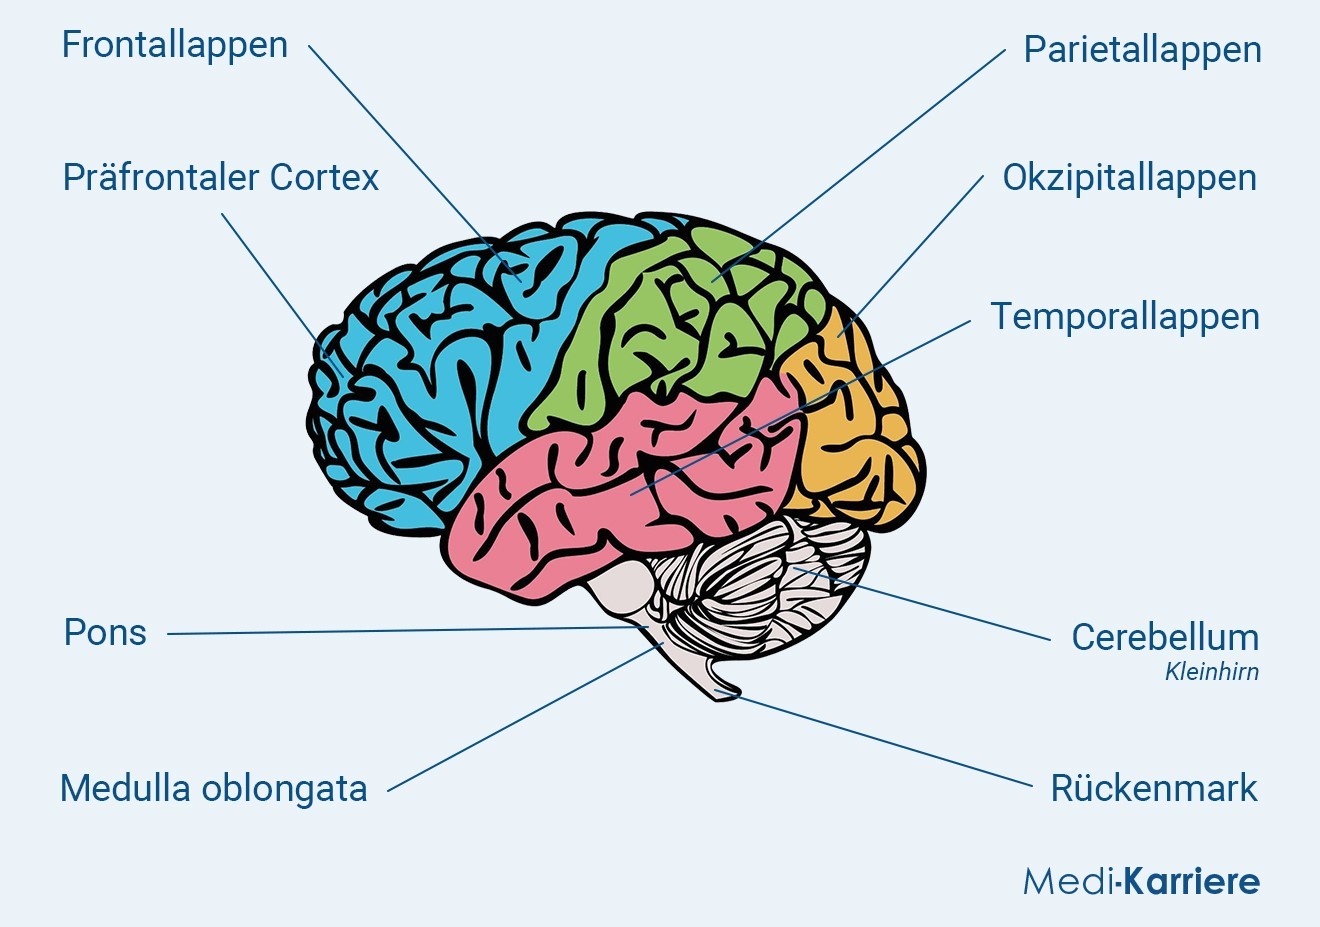
\includegraphics[width=0.65\textwidth]{bilder/Hirnaufbau.jpg}
    \quelle{\cite{medi_cortex}.} 
   \caption{Schematische Darstellung der Cortexareale}
    \label{Hirnaufbau}
\end{figure}
Der Lobus frontalis (Frontallappen) liegt am vorderen Hirnpol an und erstreckt sich bis zum Beginn des Lobus parietalis (Parietallappen). Somit ist er der größte Teil des Cerebrums. Der Lobus frontalis ist an wichtigen Funktionen wie der Motorik und an komplexen Funktionen beteiligt.\footnote{Vgl. \cite{elbaba2023_frontal}} Zum einen bildet er den Ursprung motorischer Bewegungen und dient dazu, komplexe Bewegungsabläufe zu planen und durchzuführen. Zu den komplexen Funktionen gehören vor allem hohe kognitive Leistungen, wie bspw. Rechnen, Schreiben und Planen.\footnote{Vgl. \cite{elbaba2023_frontal}} Des Weiteren ist er an ethischem Verhalten und an Emotionen beteiligt.

Besonders wichtig ist der präfrontale Cortex. Er bildet den vorderen Teil des Lobus frontalis und empfängt sensorische Signale und steht in Zusammenhang mit der Integration von Gedächtnisinhalten und emotionalen Bewertungen. Weitere wichtige Funktionen sind das Arbeitsgedächtnis und die Planung zukünftiger Handlungen.\footnote{Vgl. \cite{elbaba2023_frontal}}

An den Lobus frontalis grenzt am oberen, hinteren Teil des Gehirns der Lobus parietalis an. Der Parietallappen ist für die Verarbeitung sensorischer Eindrücke verantwortlich und spielt eine zentrale Rolle bei der somatosensorischen Wahrnehmung.\footnote{Vgl. \cite{javed2023_cortex}} Dazu zählen haptische Empfindungen wie Berührung, Druck und Vibration. \gls{epikrImpulse}, darunter das feine Tastempfinden sowie die Propriozeption, also die bewusste Wahrnehmung der Körperlage im Raum, werden an weitere Gehirnareale des Lobus parietalis weitergeleitet und dort verarbeitet. \gls{ProtoImpulse} wie Schmerz- und Temperaturreize werden ebenfalls sensorisch erfasst. Zudem ist der Lobus parietalis an der Verarbeitung visueller Reize beteiligt.\footnote{Vgl. \cite{javed2023_cortex}}

Im hinteren Teil des Cerebrums und an den Lobus parietalis angrenzend liegt der Lobus occipitalis (Okzipitallappen). Dieser enthält größtenteils die Sehrinde; diese ist vor allem für die visuelle Informationsverarbeitung zuständig. Innerhalb der Sehrinde erfolgt die Verschaltung visueller Eindrücke, wobei jeder Bereich der Sehrinde einem spezifischen Bildausschnitt des visuellen Feldes zugeordnet ist. Das ermöglicht es dem Gehirn, gezielt anvisierte Punkte im Blickfeld zu fokussieren und visuelle Details zu erkennen. So wird eine differenzierte Wahrnehmung und eine genaue Fokussierung auf Objekte im Raum ermöglicht.\footnote{Vgl. \cite{rehman2023_occipital}}

Der vierte Lobus cerebri, der Lobus temporalis (Temporallappen), bildet den seitlichen Anteil des Cerebrums und grenzt an alle drei Lobi an.\footnote{Vgl. \cite{kenhub_temporallappen}}

Der Lobus temporalis ist der zweitgrößte Großhirnlappen und übernimmt eine zentrale Rolle in der auditiven Wahrnehmung. Dort werden die von den Sinneszellen der Hörschnecke weitergeleiteten Signale verarbeitet. Zusätzlich befindet sich im Lobus temporalis das \gls{wernick}; dieses dient \glqq der semantischen Verarbeitung und Integration von Sprach- und Textinhalten\grqq{}.\footnote{\cite{doccheck_wernicke}}

\section{Entstehung und Weiterleitung elektrischer Signale im Gehirn}

\subsection{Grundlegende Entstehung und Weiterleitung}
\label{sec:entstehung}
\autor{Alisa Fiedler}

Das Gehirn ist das größte Organ des menschlichen Nervensystems und gehört zum zentralen Nervensystem.\footnote{Vgl. \cite{hescheler2010}} Es ist über das \Gls{rückenmark} und das \gls{periphere Nervensystem} mit dem ganzen Körper verbunden und übernimmt Funktionen wie die Verarbeitung von Informationen, die Integration von Sinnesreizen, die Koordination von Bewegungen und die Regulierung lebensnotwendiger Prozesse.\footnote{Vgl. \cite{maldonado2023_brain}} Die zuvor behandelten Strukturen des Gehirns bilden dabei die anatomische Grundlage für diese Funktionen. Damit diese Strukturen aktiv miteinander arbeiten können, ist eine Kommunikation notwendig.

\begin{figure}[H]
	\centering
	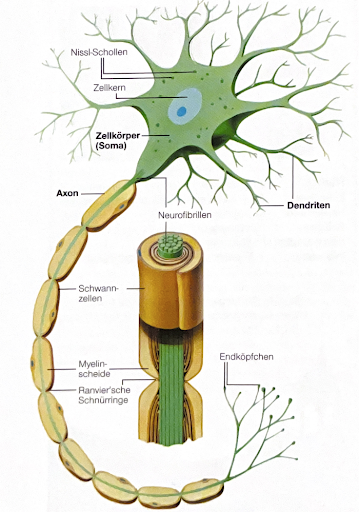
\includegraphics[width=0.4\textwidth]{bilder/Neuron.png}
    \quelle{\cite{varnhorn_2005}.}
    \caption{Aufbau eines Neurons}
    \label{Neuron}
\end{figure}

Diese Kommunikation wird von den Nervenzellen, den Neuronen (vgl. Abbildung~\ref{Neuron}), ermöglicht. Das Gehirn setzt sich aus Milliarden von Nervenzellen zusammen. Erst durch ihre Vernetzung bilden sich Netzwerke, die Informationen schnell aufnehmen und verarbeiten können. Neuronen haben sich auf die Erregungsleitung und -weitergabe spezialisiert.\footnote{Vgl. \cite{ludwig2023_neurons}}

Zellkörper und mehrere Fortsätze mit unterschiedlichen Funktionen bilden die Bestandteile von Nervenzellen. Die Dendriten empfangen Signale von Neuronen und transportieren sie weiter zum Soma (Zellkörper), wo die eingehenden Signale weiterverarbeitet werden. Vom Soma aus verläuft das Axon (Nervenfaser), das elektrische Signale in Form von Aktionspotenzialen zu Nerven- oder Muskelzellen weiterführt. Die synaptischen Endknöpfchen liegen am Ende des Axons. Sie enthalten Neurotransmitter (biochemische Substanzen), die Reize an die nächste Zelle weitergeben.\footnote{Vgl. \cite{studyflix_synapse}} Die Axone sind funktionell mit anderen Zellen verbunden, was die Zell-Zell-Kommunikation ermöglicht.

Die Grundlage für jedes elektrische Signal einer Nervenzelle ist das Ruhepotenzial. Es handelt sich hierbei um die elektrische Spannung zwischen der Innen- und Außenseite einer nicht erregten Zelle. Dieses Membranpotenzial beträgt bei einer Nervenzelle etwa $-70$\,mV, wobei der Innenraum der Zelle negativ und das Zelläußere positiv geladen ist. Ursache dafür ist die ungleiche Verteilung von Natrium- (Na$^+$), Kalium- (K$^+$) und Chlorid-Ionen (Cl$^-$) sowie organischen Anionen.\footnote{Vgl. \cite{hescheler2010}}

Innerhalb der Zelle befindet sich das Cytoplasma. Dort ist die Konzentration an Kalium-Ionen (K$^+$) und organischen Anionen hoch. Die Zellmembran ist semipermeabel, was bedeutet, dass sie den Zellinnenraum vom Äußeren abgrenzt. Darüber hinaus ist sie unterschiedlich durchlässig für verschiedene Ionen. Insbesondere Kaliumionen können die Membran über offene Kanäle passieren, während Natriumionen nur in geringem Maß eindringen können. Diese selektive Permeabilität führt zur Bildung eines Konzentrationsgradienten, der die Ionendiffusion antreibt, sowie eines elektrischen Gradienten, der aus der Ladungstrennung entsteht. Der Ionenkonzentrationsgradient entsteht durch die zufällige Brownsche Molekularbewegung vom Ort höherer Konzentration zum Ort niedriger Konzentration durch die Diffusion. Der elektrische Gradient dagegen entsteht, wenn die Ladung zu- oder abnimmt, wenn sich Ionen aus der Zelle ein- oder herausbewegen. Durch die Ladungstrennung bildet sich ein elektrisches Feld und es entsteht eine Spannung über der Membran. Die elektrische Kraft wirkt der weiteren Bewegung gleich geladener Ionen entgegen und zieht entgegengesetzte Ladungen an, wodurch sich zwischen beiden Kräften ein Gleichgewicht einpendelt.\footnote{Vgl. \cite{studyflix_ruhepotential}}

Das Gleichgewicht zwischen dem Konzentrationsgradienten der Ionen und dem elektrischen Gradienten führt zur Stabilisierung des Ruhemembranpotenzials
\begin{figure}
	\centering
	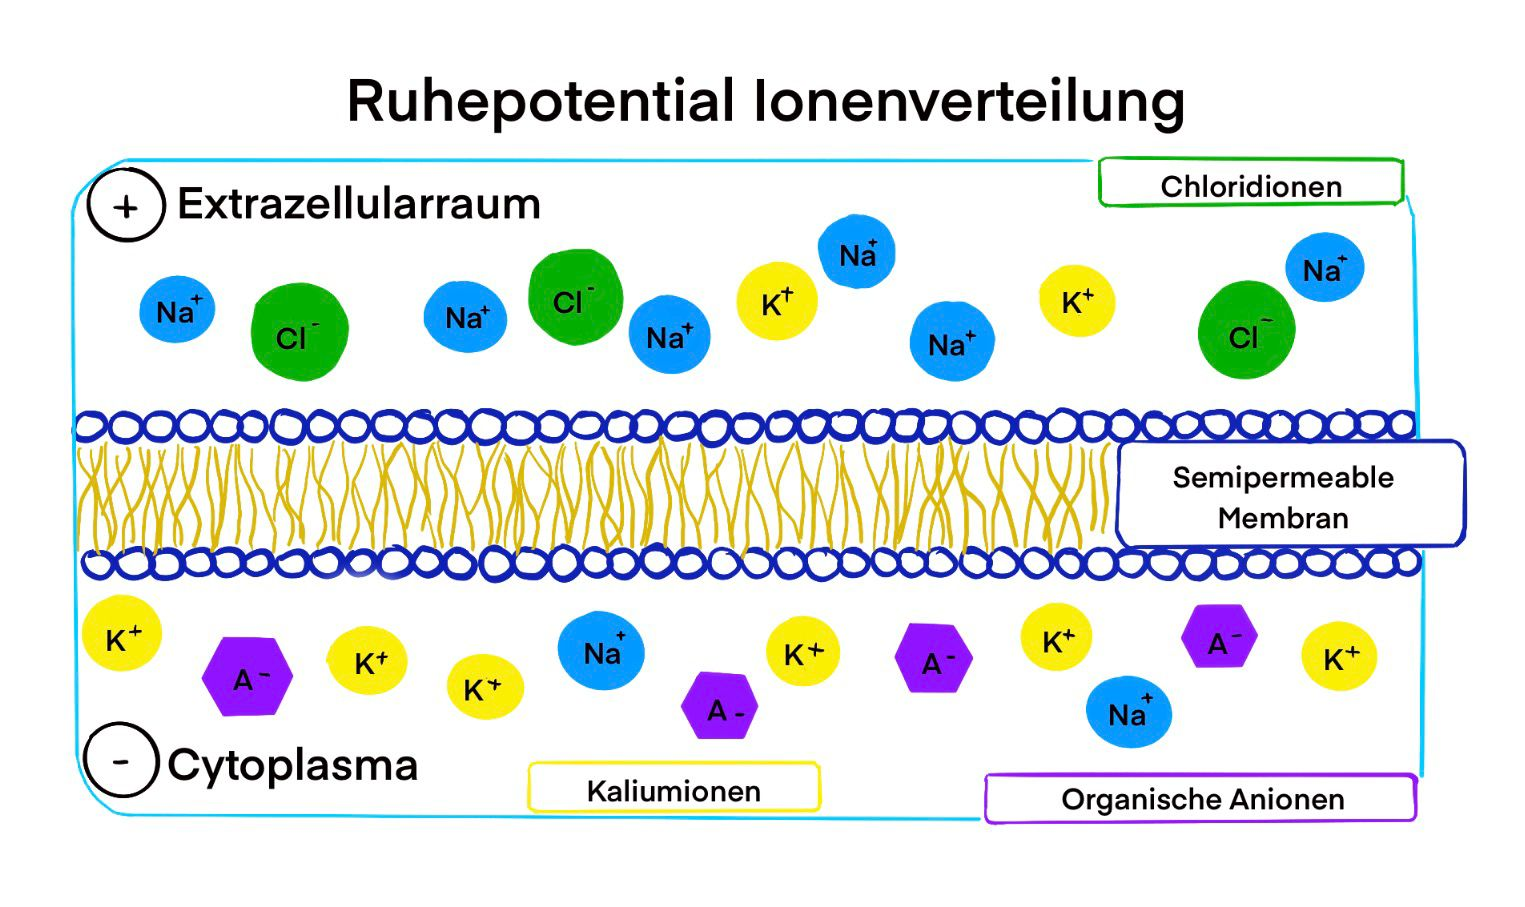
\includegraphics[width=0.7\textwidth]{bilder/ruhepotential_ionenverteilung.jpeg}
    \quelle{Eigene Abbildung in Anlehnung an \cite{studyflix_Abbildung}.}
    \caption{Ionenverteilung an einem Neuron während des Ruhepotenzials}
    \label{Ruhepotenzial}
\end{figure}
(Abbildung \ref{Ruhepotenzial}). Damit das Ruhepotenzial aufrechterhalten bleibt, spielt die Natrium-Kalium-Pumpe eine entscheidende Rolle. Das Enzym Natrium-Kalium-ATPase transportiert Natriumionen aus der Zelle hinaus und Kaliumionen in das Zytoplasma hinein. Dabei wird Energie in Form von Adenosintriphosphat (ATP) benötigt.\footnote{Vgl. \cite{hescheler2010}} Dadurch werden die Ionenkonzentrationen aufrechterhalten und Leckströme ausgeglichen, wodurch das Ruhepotenzial stabilisiert wird. Als Leckstrom bezeichnet man den kontinuierlichen, passiven Ionentransport über die Zellmembran von Neuronen. Dabei diffundieren Natriumionen trotz der geringen Durchlässigkeit der Membran in die unerregte Nervenzelle. Dies passiert aufgrund des Konzentrationsgefälles und der Ladungsverhältnisse. Leckströme würden langfristig das Ruhepotenzial aufheben, weshalb die Natrium-Kalium-Pumpe dieses Phänomen verhindert.\footnote{Vgl. \cite{wiki_leckstrom}}

Trifft ein ausreichend starker Reiz auf eine Nervenzelle, so kommt es zur Entstehung eines Aktionspotenzials. Das Aktionspotenzial ist die vorübergehende Spannungsänderung des Membranpotenzials über die Zellmembran.\footnote{Vgl. \cite{studyflix_refraktaerzeit}} Seine Funktion ist die Reizweiterleitung zwischen den Nervenzellen. Wird am Axonhügel der Schwellenwert von etwa $-50$\,mV überschritten, so kommt es zu einer Öffnung von Natriumkanälen. Anschließend strömt Natrium in die Zelle hinein, wodurch das Membranpotenzial auf etwa $+30$\,mV ansteigt (Depolarisation). Nachfolgend schließen sich die Natriumkanäle und Kaliumkanäle öffnen sich, sodass Kalium aus der Zelle fließt (Repolarisation). Danach kommt es zu einer Hyperpolarisation, bevor das Ruhepotenzial wiederhergestellt wird. Dabei schließen sich die Kaliumkanäle wieder. Darauffolgend findet die Rückkehr zum Ruhepotenzial statt, bei der die Natrium-Kalium-Pumpe das Ausgangspotenzial wiederherstellt.\footnote{Vgl. \cite{kenhub_aktionspotential}} Das Alles-oder-Nichts-Prinzip besagt, dass es keine halben oder unterschiedlich starken Aktionspotenziale gibt. Das bedeutet, dass alle Aktionspotenziale immer gleich stark sind.

\begin{figure}[H]
	\centering
	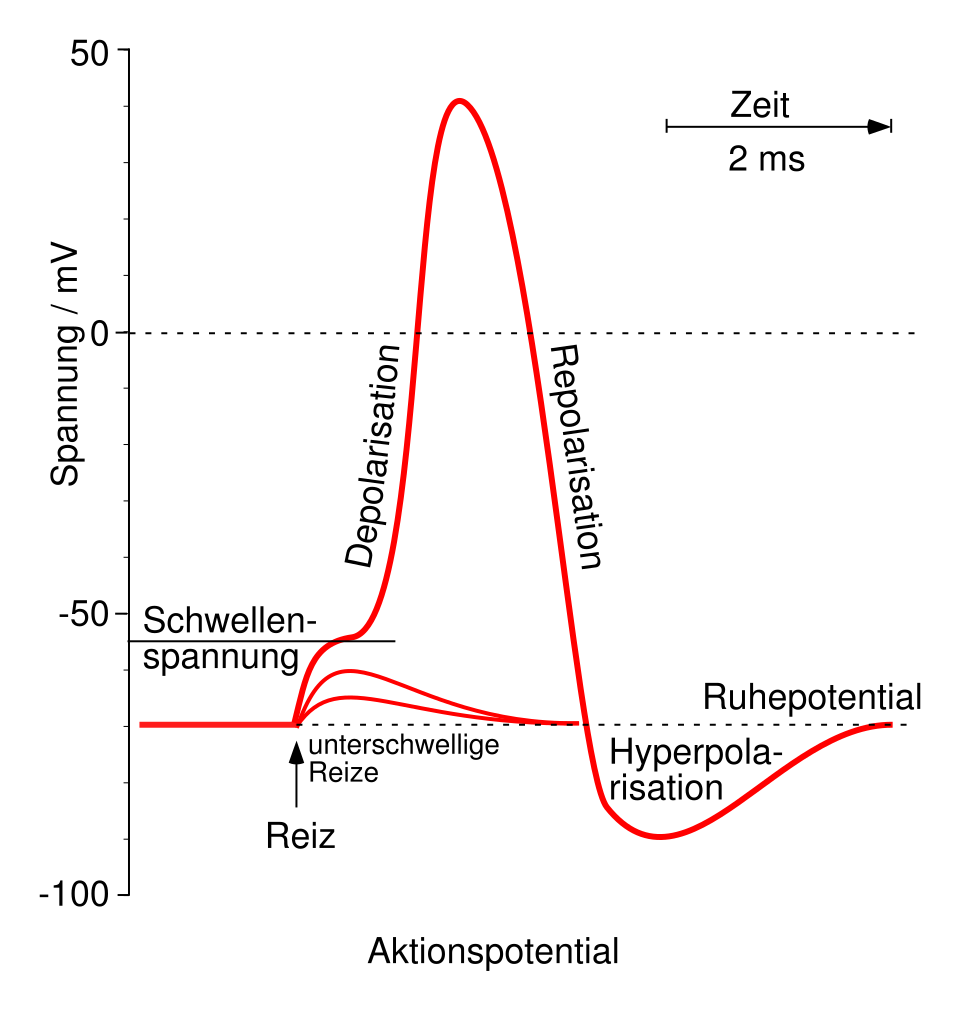
\includegraphics[width=0.625\textwidth]{bilder/Aktionspotential.svg}
    \quelle{\cite{wiki_aktionspotential}.}
    \caption{Der zeitliche Verlauf der Spannung während einer Erregung (Aktionspotenzial)}
    \label{Aktionspotenzial}
\end{figure}
Das Aktionspotenzial (Abbildung~\ref{Aktionspotenzial}) ist für den menschlichen Körper von zentraler Bedeutung, da es die Grundlage der neuronalen Kommunikation darstellt. Es ermöglicht die schnelle Signalübertragung entlang von Nervenzellen.\footnote{Vgl. \cite{studyflix_refraktaerzeit}} Zudem ist es notwendig, Reize, wie Berührung, Schmerz oder Temperatur, zu spüren sowie Muskeln gezielt zu bewegen. Darüber hinaus bildet das Aktionspotenzial die grundlegende Kommunikationsform im Körper und ermöglicht den Austausch von Informationen zwischen Gehirn, Rückenmark und inneren Organen.\footnote{Vgl. \cite{hescheler2010}}

Das Aktionspotenzial wird entlang des Axons weitergeleitet und ermöglicht so die schnelle Informationsübertragung innerhalb des Neurons. Um Informationen weiterzuleiten, ist eine Übertragung an Synapsen notwendig. Eine Synapse, also eine Verbindungsstelle zwischen Nervenzellen, ist \glqq eine Kontaktstruktur zur Übertragung eines chemischen oder elektrischen Signals von einer Nervenzelle auf eine andere Nervenzelle\grqq{}.\footnote{\cite{doccheck_synapse}} Die Synapse ist aus einer Präsynapse, der Postsynapse und dem dazwischenliegenden synaptischen Spalt aufgebaut.\footnote{Vgl. \cite{studyflix_synapse}}

Man unterscheidet elektrische und chemische Synapsen. Elektrische Synapsen bestehen aus direkten Zellverbindungen (Gap Junctions), durch die Ionen und niedermolekulare Substanzen unmittelbar von einer Nervenzelle durch Ionenkanäle zur nächsten fließen. Sie ermöglichen eine sehr schnelle Signalübertragung, welche in beide Richtungen möglich ist.

Häufiger sind jedoch chemische Synapsen. Trifft ein Aktionspotenzial an der Präsynapse ein, so kommt es zu einer Spannungsänderung in der präsynaptischen Membran. Es öffnen sich Calciumkanäle und es folgt ein Einströmen von Calcium-Ionen in die Zelle. Dies führt dazu, dass Vesikel mit Neurotransmittern mit der präsynaptischen Membran verschmelzen und ihre Botenstoffe in den synaptischen Spalt freisetzen. Die Neurotransmitter binden an spezifische Rezeptoren und öffnen dort Ionenkanäle. Von dort aus strömen Natriumionen aus dem Spalt in die Postsynapse, dadurch kommt es zu einer Spannungsänderung in der postsynaptischen Membran und zur Weiterleitung des Aktionspotenzials. Die Transmitter lösen sich anschließend wieder vom Rezeptor und werden von der Präsynapse aufgenommen oder enzymatisch abgebaut und bei der nächsten Reizweiterleitung wiederverwendet.\footnote{Vgl. \cite{studyflix_synapse}} Je nach Art der Synapse hat die Signalübertragung unterschiedliche Auswirkungen auf die Zielzelle. Erregende Synapsen lösen in der postsynaptischen Zelle ein exzitatorisches postsynaptisches Potenzial aus (kurz \acrshort{epsp}). Dies führt zu einer Depolarisation der Zellmembran und erhöht die Wahrscheinlichkeit, dass das Signal weitergeleitet wird und in der Zielzelle ein neues Aktionspotenzial entsteht. Hemmende Synapsen erzeugen hingegen ein inhibitorisches postsynaptisches Potenzial (\acrshort{ipsp}). Dabei kommt es zu einer Hyperpolarisation der postsynaptischen Membran, wodurch die Entstehung eines Aktionspotenzials erschwert oder verhindert wird und die Signalweiterleitung gehemmt wird.\footnote{Vgl. \cite{studyflix_epsp_ipsp}}

Einzelne Aktionspotenziale sind sehr kurz und lokal begrenzt und daher nicht direkt messbar. Messbar hingegen sind länger anhaltende postsynaptische Potenziale vieler Nervenzellen, die parallel zueinander liegen. Durch die gleichzeitige Aktivität einer großen Neuronengruppe entsteht ein Dipol, der an der Kopfoberfläche messbar ist. Die Aktivierung mehrerer solcher Gruppen erzeugt rhythmische Spannungsänderungen, die als Gehirnwellen bezeichnet werden. 

\subsection{Saltatorische Erregungsleitung}
\autor{Lorenz Kobylka}

Das Axon ist von einer isolierenden Myelinscheide umgeben, die seine Funktion maßgeblich unterstützt. Im Nervensystem spielen die Myelinscheiden eine zentrale Rolle bei der schnellen und effizienten Erregungsleitung. Diese Myelinscheiden werden im peripheren Nervensystem von den Schwannschen Zellen und im zentralen Nervensystem von den \gls{oligo} gebildet.\footnote{Vgl. \cite{grider2026_ranvier}} Die Myelinscheiden erfüllen mehrere wichtige Funktionen, wie die elektrische Isolation der Axone, die Versorgung der Nervenfasern und den physischen Schutz. Ein charakteristisches Merkmal dieser Myelinscheiden ist der Ranviersche Schnürring, ein Bereich zwischen den Myelinscheiden, der nicht isoliert ist. Dieser nicht-myelinisierte Abschnitt hat eine Länge von etwa 1\,µm und ermöglicht die sogenannte saltatorische Erregungsleitung.\footnote{Vgl. \cite{grider2026_ranvier}} Diese ermöglicht, dass ein Aktionspotenzial sprunghaft von einem Schnürring zum nächsten weitergeleitet wird, und leitet sich vom lateinischen Begriff \textit{\glqq saltare\grqq{}} (springen) ab.

Wenn ein Aktionspotenzial den Ranvierschen Schnürring erreicht, öffnen sich spannungsgesteuerte Natrium-Ionenkanäle. Dies hat zur Folge, dass $Na^+$-Ionen aus dem extrazellulären Milieu in das Axon strömen, wie schematisch in Abbildung \ref{Saltatorische Erregungsleitung} dargestellt ist. Die Axonmembran wird nun an dieser Stelle depolarisiert, also positiver.\footnote{Vgl. \cite{studyflix_erregungsleitung}} Dieses elektrische Potenzial breitet sich passiv am Axon weiter aus. Erreicht dieses Potenzial den nächsten Schnürring, öffnen sich erneut spannungsabhängige Natrium-Ionenkanäle und $Na^+$-Ionen strömen in das Axon. Es entsteht ein neues Aktionspotenzial.\footnote{Vgl. \cite{studyflix_erregungsleitung}}

Nach der Entstehung eines Aktionspotenzials öffnen sich spannungsabhängige Kalium-Ionenkanäle, wodurch $K^+$-Ionen aus dem Axon ausströmen. Dieser Ausstrom von $K^+$-Ionen führt dazu, dass das Membranpotenzial wieder negativer wird und sich dem Ruhepotenzial annähert (Repolarisation). Gleichzeitig befindet sich der zuvor erregte Schnürring in der Refraktärzeit. In dieser Phase sind die am Aktionspotenzial beteiligten Ionenkanäle vorübergehend inaktiviert, sodass an dieser Stelle kein neues Aktionspotenzial ausgelöst werden kann. So wird sichergestellt, dass das Aktionspotenzial nur in eine Richtung weitergeleitet wird.\footnote{Vgl. \cite{studyflix_refraktaerzeit}} 

\begin{figure}[H]
	\centering
	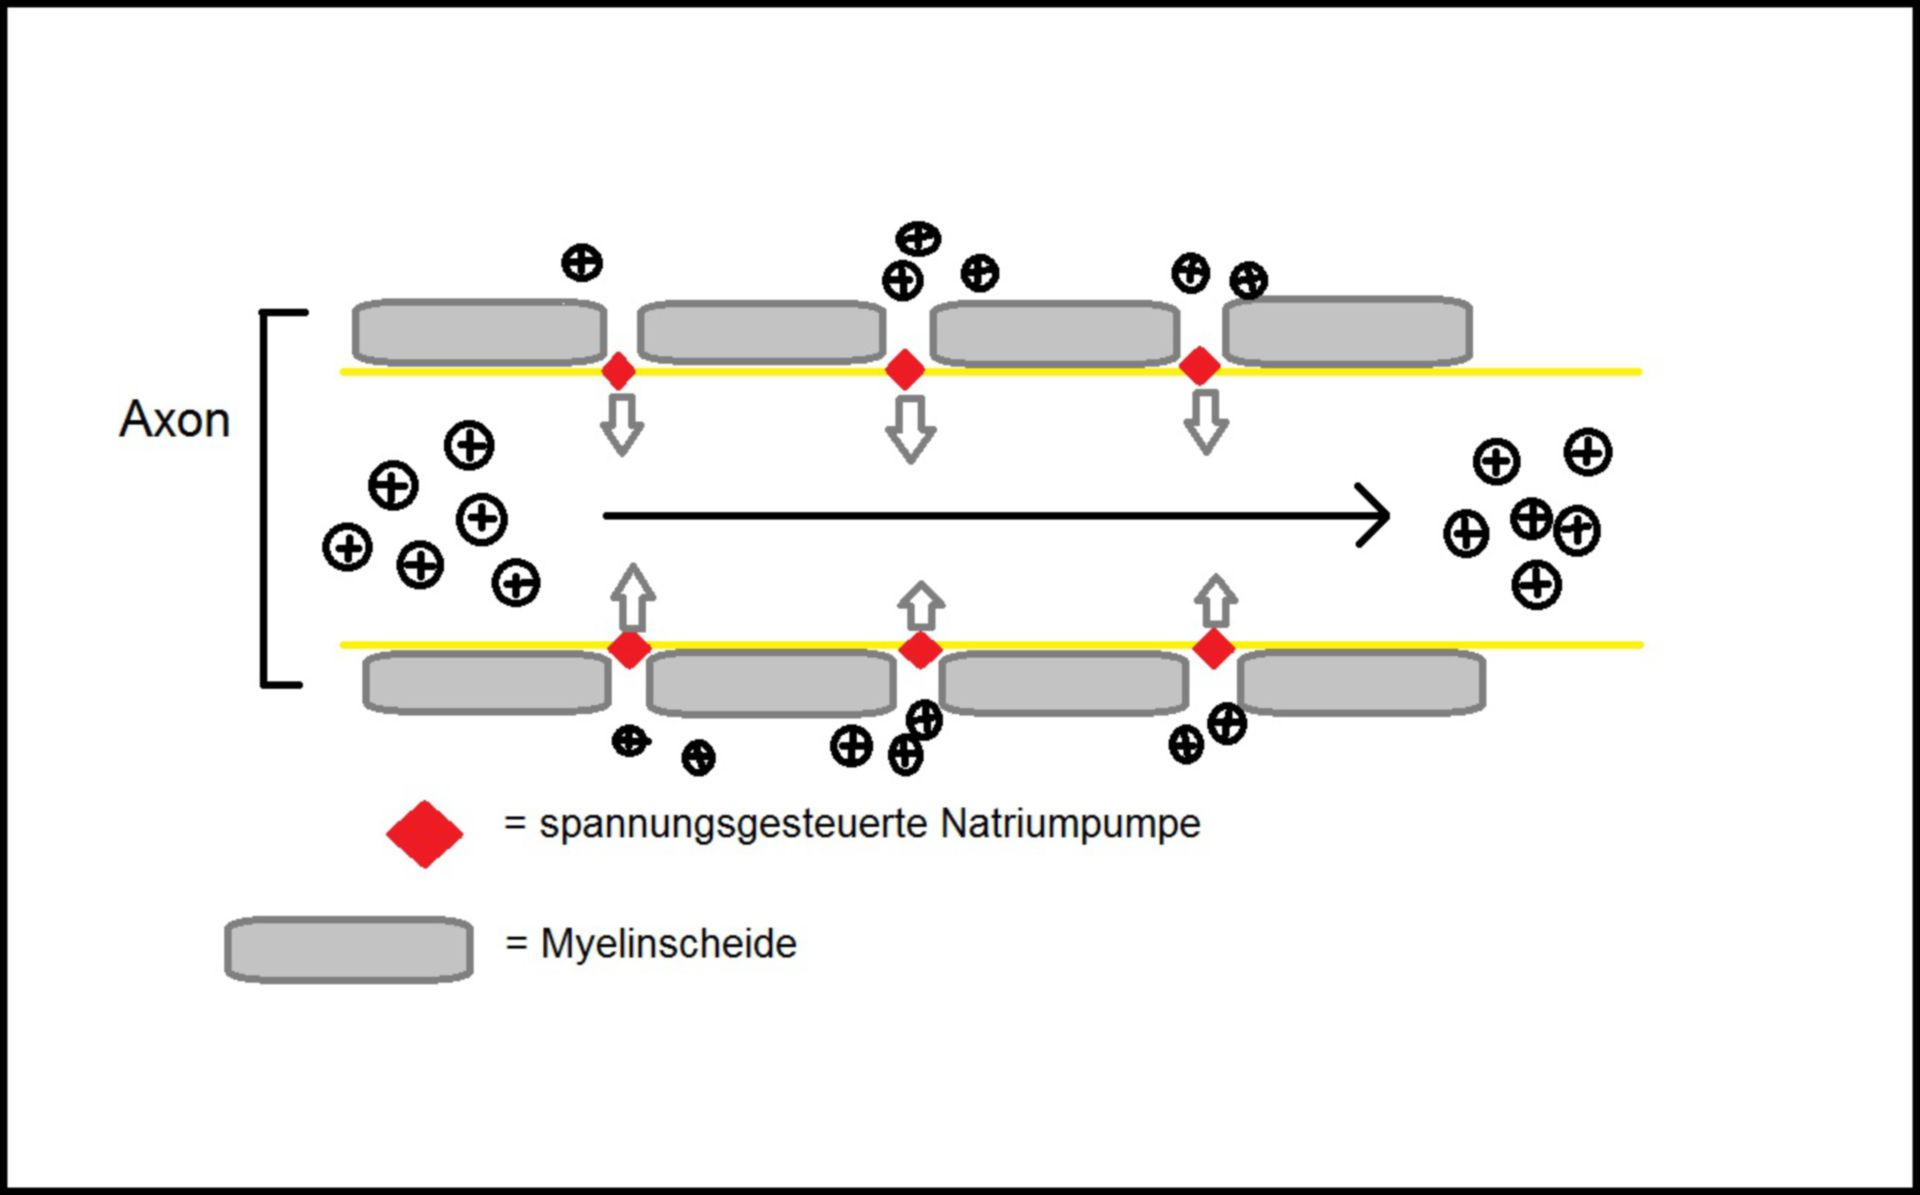
\includegraphics[width=0.65\textwidth]{bilder/Erregungsleitung.jpg}
    \quelle{\cite{doccheck_saltatorisch}.}    
    \caption{Schematische Darstellung der saltatorischen Erregungsweiterleitung}
    \label{Saltatorische Erregungsleitung}
\end{figure}

\subsection{Neuronale Verrechnung}
\autor{Lorenz Kobylka}

Jedes Neuron ist mit einer Vielzahl von Synapsen mit anderen Neuronen verbunden. Somit treffen in einem Neuron kontinuierlich zahlreiche Signale über Synapsen ein, die darüber entscheiden, ob ein Aktionspotenzial ausgelöst wird oder nicht. Diese Signale sind entweder erregend (\acrshortpl{epsp}) oder hemmend (\acrshortpl{ipsp}, vgl. Abschnitt~\ref{sec:entstehung}).\footnote{Vgl. \cite{betts2022_openstax}} Ein einzelnes \acrshort{epsp} reicht in der Regel nicht aus, um den Schwellenwert für die Auslösung eines Aktionspotenzials zu überschreiten. Daher ist eine Verrechnung mehrerer Signale notwendig. Diese Verrechnung erfolgt am Axonhügel des Neurons, dort werden die \acrshortpl{epsp} und \acrshortpl{ipsp} summiert (vgl. Abbildung~\ref{IPSP}). Übersteigt diese Summe einen bestimmten Schwellenwert, unter Berücksichtigung der hemmenden Signale, wird ein Aktionspotenzial am Axonhügel ausgelöst.\footnote{Vgl. \cite{betts2022_openstax}}

Dabei unterscheidet man zwei Formen der Summation: die zeitliche und die räumliche Summation. Bei der zeitlichen Summation addieren sich mehrere \acrshortpl{ipsp} oder \acrshortpl{epsp}, die in kurzen Abständen an die Synapse übertragen werden. Wenn sich \acrshortpl{ipsp} zeitlich summieren, wird das Membranpotenzial des folgenden Neurons zunehmend negativer (Hyperpolarisation). Das bedeutet, dass sich das Membranpotenzial weiter vom Schwellenwert entfernt.\footnote{Vgl. \cite{examio_summation}} Wenn sich hingegen \acrshortpl{epsp} zeitlich summieren, wird das Membranpotenzial des folgenden Neurons zunehmend positiver (Depolarisation). Dadurch steigt die Wahrscheinlichkeit, dass der Schwellenwert für ein Aktionspotenzial übertroffen wird.\footnote{Vgl. \cite{examio_summation}} Die zweite Form der Summation ist die räumliche Summation. Diese beschreibt das gleichzeitige Eintreffen von Signalen an verschiedenen Synapsen. Dabei werden mehrere \acrshortpl{epsp} oder auch eine Mischung aus \acrshortpl{epsp} und \acrshortpl{ipsp} gleichzeitig verrechnet.\footnote{Vgl. \cite{examio_summation}} Ausschlaggebend ist dabei die Entfernung der Synapse zum Axonhügel. Signale, die näher am Axonhügel übertragen werden, haben einen stärkeren Einfluss auf die Entstehung eines Aktionspotenzials. Beispielsweise treffen entfernt vom Axonhügel viele \acrshortpl{epsp} ein, während nahe am Axonhügel ein \acrshort{ipsp} eintrifft. In diesem Fall kann es passieren, dass der Schwellenwert nicht überschritten wird. Zusammenfassend lässt sich sagen, dass die Entstehung eines Aktionspotenzials das Ergebnis einer komplexen Verrechnung von erregenden und hemmenden Einflüssen ist. Nur wenn die Summe der \acrshortpl{epsp} die hemmenden Effekte der \acrshortpl{ipsp} überwiegt und der Schwellenwert am Axonhügel überschritten wird, kommt es zur Weiterleitung eines elektrischen Signals entlang des Axons.\footnote{Vgl. \cite{betts2022_openstax}}

\begin{figure}[H]
	\centering
	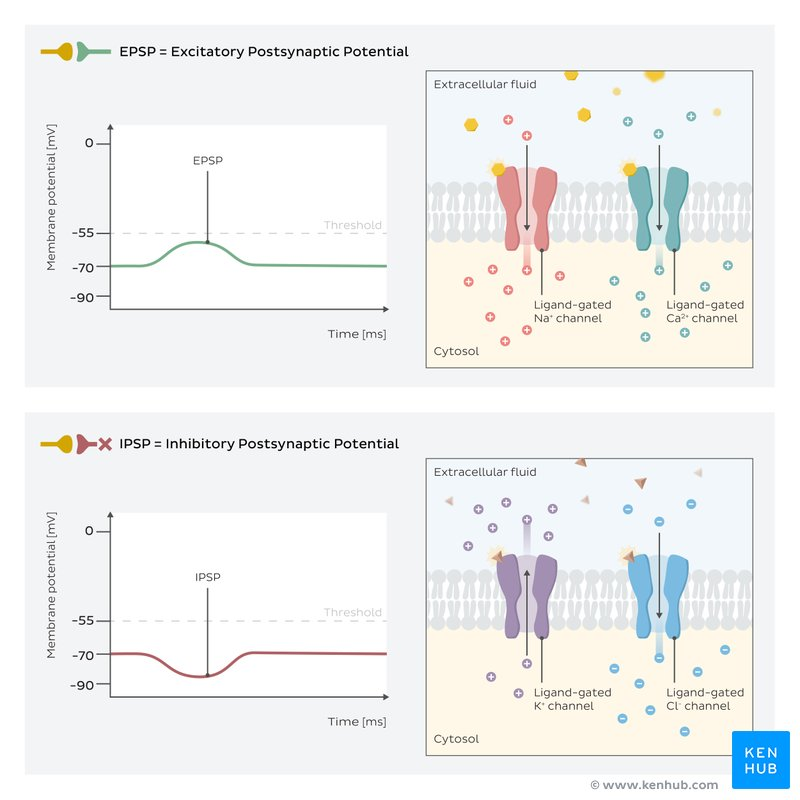
\includegraphics[width=0.65\textwidth]{bilder/ipsp.jpg}
    \quelle{\cite{kenhub_psp}.}    
    \caption{Darstellung des Einflusses eines EPSPs und IPSPs auf das Membranpotenzial}
    \label{IPSP}
\end{figure}

\section{Aufbau und Funktionsweise eines EEG-Systems}
\autor{Katharina Ensslen}
\subsection{Grundlegende Messmethode eines EEG-Systems}
Die entstehenden postsynaptischen Potenziale vieler gleichzeitig aktiver Neuronen haben messbare lokale Spannungsänderungen im Gehirn zur Folge (vgl. Abschnitt~\ref{sec:entstehung}). Das \acrshort{eeg} hat das Ziel, diese elektrischen Gehirnaktivitäten zu erfassen und aus ihnen Rückschlüsse auf Verarbeitungsprozesse im Gehirn zu ziehen. Hierzu werden die Spannungsdifferenzen auf der Kopfhaut mithilfe von Elektroden gemessen.

Eine Elektrode ist ein elektrischer Leiter, der zusammen mit einer Gegenelektrode mit einem Medium, das sich zwischen beiden Elektroden befindet, in Wechselwirkung steht. Elektroden bestehen meist aus Metall oder Graphit und ermöglichen die Messung von Spannungsunterschieden.\footnote{Vgl. \cite{heinen_elektronik_elektroden}}

Werden zwei Elektroden nah an der Kopfhaut angebracht, erfassen sie die Spannungsdifferenz zwischen den jeweiligen Messorten. Beide Elektroden messen nicht nur die Spannung, die durch Gehirnaktivität entstand, sondern weitere Spannungen, die unabhängig von der Aktivität aufgrund elektrischer Geräte in der Umgebung erzeugt werden. Wird eine Elektrode an einem Ort angebracht, an dem möglichst wenig Hirnaktivität zu messen ist, entspricht die Spannungsdifferenz näherungsweise der durch Gehirnaktivität an der anderen Elektrode erzeugten Spannung. Einen vollständig neutralen Punkt gibt es am Körper allerdings nicht, was als \gls{no-switzerland-principle} bezeichnet wird (vgl. Abschnitt~\ref{sec:stoer}).
Auf diese Weise lässt sich die Gehirnaktivität in der Umgebung einer Elektrode über längere Zeiträume hinweg aufzeichnen. Durch den Einsatz mehrerer Elektroden können Signale aus unterschiedlichen Hirnregionen gleichzeitig erfasst werden, wobei sich die gemessenen Muster je nach Funktion der jeweiligen Region unterscheiden. Die Aufzeichnungen lassen sich durch Weiterverarbeitung in interpretierbare Muster übersetzen. Mit diesen Informationen können Rhythmen bestimmt und bestimmte Aktivitäten provoziert werden.

Eine Einschränkung beim \acrshort{eeg} ist die räumliche Auflösung. Die elektrischen Signale entstehen in Nervenzellen, über einen Zentimeter von der Kopfhaut entfernt, während die Messung an der Kopfhaut erfolgt. Zwischen diesen Orten liegt eine räumliche Distanz, auf dem sich die Signale verbreiten. Außerdem erzeugen nur große Flächen gleichzeitig aktiver Neuronen messbare Signale. Die Elektroden messen demnach nicht nur die Spannung eines einzelnen Punktes, sondern einer Fläche von mindestens 6\,cm$^2$ der Oberfläche des Gehirns, über deren Zentrum sich die Elektrode befindet.\footnote{Vgl. \cite[Appendix~1]{stlouis2016}} Dieser Umstand hat zur Folge, dass empfangene Signale nicht örtlich einzuordnen sind. Daher ist die räumliche Auflösung von Hirnsignalen mit \acrshort{eeg} nur eingeschränkt bestimmbar. Im Gegensatz dazu ist jedoch die zeitliche Einordnung sehr exakt. Das bedeutet, dass zwischen dem Zeitpunkt, an dem Neuronengruppen aktiviert werden, und dem, an dem das elektrische Signal die Elektroden erreicht und aufgezeichnet wird, nahezu keine Zeit (ungefähr 1 ms)\footnote{Vgl. \cite{tu_darmstadt2022}} vergeht. 

\subsection{Geschichte und aktueller Stand der Forschung}
Richard Caton hat als Erster Messungen von Gehirnaktivität durchgeführt. Er zeigte in Liverpool, dass Gehirne von Affen und Kaninchen elektrische Ströme erzeugen, die durch Sinnesreize beeinflusst werden. Als \qt{Entdecker der Elektroenzephalographie} gilt jedoch ein Neurologe aus Jena. Hans Berger führte 1924 die ersten Elektroenzephalographien an der Universität Jena durch. Er entdeckte auch den \gls{berger-effekt}, eine leicht stimulierbare Veränderung des \acrshort{eeg}s, die auffällig und damit leicht messbar ist.\footnote{Vgl. \cite{caeira2023_berger}}

Seit der Entwicklung des ersten \acrshort{eeg} haben zahlreiche Institutionen, Unternehmen und Forschende daran gearbeitet, sowohl die Messgenauigkeit zu verbessern als auch neue Einsatzmöglichkeiten zu erschließen. Dabei lassen sich die Fortschritte und Anwendungen des \acrshort{eeg} nach unterschiedlichen Anwendungsbereichen strukturieren.

Ein zentraler Fokus liegt auf der Verbesserung der Messqualität, da genauere Daten die Grundlage für alle weiteren Anwendungen bilden. Durch Anpassungen an verschiedenen Komponenten des \acrshort{eeg}-Geräts können Abweichungen von der tatsächlichen Gehirnaktivität reduziert werden. Ein besonders fortschrittliches System (Stand 2023) stammt von Neuroscan und wird häufig in der Industrie eingesetzt, da es sowohl in Hard- als auch Software vielen anderen \acrshort{eeg}-Geräten überlegen ist. Auch Brain Products, ein deutsches Unternehmen, hat zur Weiterentwicklung beigetragen, etwa durch die Entwicklung eines \acrshort{eeg}-Headsets mit 160 Elektroden. Dieses ist deutlich dichter als herkömmliche Systeme, die meist maximal 128 Elektroden verwenden.

Ein wichtiger Anwendungsbereich sind sogenannte \Glspl{brain-computer-interface} (\acrshort{bci}). Hierbei wird die Gehirnaktivität erfasst, analysiert und in Steuersignale umgewandelt. Systeme wie das von NeuSen W wurden gezielt für diesen Zweck entwickelt. \acrshortpl{bci} stellen somit eine konkrete Anwendung der Neurotechnik dar.
\acrshort{eeg}-basierte \acrshort{bci}-Technologien finden besonders im medizinischen Bereich Verwendung. Dazu zählen unter anderem Rehabilitation, Epilepsie-Diagnostik, Emotionserkennung und neurodegenerative Erkrankungen wie Alzheimer und Parkinson.\footnote{Vgl. \cite{liu2025}} Durch die Auswertung von Gehirnaktivität eröffnen sich vielfältige Möglichkeiten: So könnten gelähmte Körperteile wieder nutzbar gemacht, Texte ohne Muskelbewegung geschrieben oder Schlafstörungen erkannt werden.\footnote{Vgl. \cite[S.~14]{liu2025}}

Im militärischen Bereich werden \acrshortpl{eeg} beispielsweise zur Beurteilung von Schädel-Hirn-Traumata infolge von Unfällen eingesetzt.\footnote{Vgl. \cite{fanter1986}}

Einige Anwendungen befinden sich noch in der Entwicklung, da sie eine noch höhere Messgenauigkeit erfordern. Dennoch gibt es bereits heute realisierbare Ansätze. Ein Forschungsteam der Tsinghua-Universität entwickelte ein \acrshort{bci} mit einer Genauigkeit von etwa 80\,\%, mit dem ein Roboterarm gesteuert werden konnte.\footnote{Vgl. \cite[S.~3]{qin2023}} Durch gezielte Veränderung eines einzelnen Gemütszustands gelang es, Hindernisse zu umgehen und Objekte zu greifen.

\subsection{Einteilung der Geräte}
Um einen Vergleich zwischen \acrshort{eeg}-Geräten zu ermöglichen, werden sie grundsätzlich nach drei Kriterien unterschieden: den Elektroden, der Art der Übertragung zur Weiterverarbeitung und dem Anwendungsbereich.

Die Elektroden können sich auf der Kopfhaut befinden, dann sind sie nicht-invasiv. Die Alternative sind invasive Elektroden, wobei sie beispielsweise ins Gewebe (tiefe Elektroenzephalographie) oder direkt auf den Cortex implantiert werden und sich innerhalb des Schädels befinden.

Anstatt einer herkömmlichen Elektrodenplatzierung und Kabeln als Verbindung nutzen drahtlose Geräte Bluetooth oder andere digitale Übertragungswege, um höhere Flexibilität, Bequemlichkeit und alternative Platzierung der Elektroden zu ermöglichen. Drahtlose Geräte können bei invasiven und nicht-invasiven \acrshortpl{eeg} eingesetzt werden.

Das letzte Kriterium zur Einordnung von Geräten, mit denen \acrshortpl{eeg} durchgeführt werden, ist der Anwendungsbereich. Die größten Bereiche sind Forschung und Kliniken. Die Geräte, die zur Forschung genutzt werden, besitzen mehr Elektroden und das Ziel ist eine hohe Präzision, um neue Erkenntnisse zu gewinnen. In Kliniken werden \acrshortpl{eeg} nach klinischen Standards durchgeführt und für medizinische Diagnosen und Überwachungen, auch über lange Zeiträume, genutzt. Dabei ist die Bequemlichkeit wichtiger als in der Forschung.\footnote{Vgl. \cite[S.~1 und 2]{qin2023}}

\subsection{Allgemeiner Aufbau der Geräte}
\acrshort{eeg}-Geräte bestehen aus vier grundlegenden Komponenten: Elektroden, Vorverarbeitungsschaltungen, \glspl{analog-digital-converter} (\acrshortpl{adc}) und Signalsteuerung und -feedback.\footnote{Vgl. \cite[S.~4]{qin2023}}
Elektroden werden in drei Kategorien unterteilt: invasiv, nicht-invasiv-nass und nicht-invasiv-trocken.

Die Nutzung von nicht-invasiven Elektroden ist ein sicherer und chirurgiefreier Ansatz. Beispiele für solche Elektroden sind Mikronadeln (Abbildung \ref{Spitze Elektroden}), die leicht in die Haut einstechen und so den Neuronen näher sind, und fingerförmige Elektroden (Abbildung \ref{Fingerelektroden}), die leicht durchs Haar dringen und angenehmer sind als Mikronadeln. Beide üben keinen Druck auf den Kopf aus und liegen direkt am Kopf an, was die Stabilität und Genauigkeit erhöht. Die elektrischen Signale sind jedoch gestreut und geschwächt, bevor sie gemessen werden, was die Qualität der aufgenommenen Daten verringert.\footnote{Vgl. \cite[S.~4--5]{qin2023}}

Trockene Elektroden bestehen aus einem leitfähigen Material wie Metall und liegen eng am Kopf an. Bei nassen Elektroden wird \glqq ein flüssiger Elektrolyt verwendet, häufig eine Salzlösung oder ein leitfähiges Gel\grqq{}.\footnote{\cite{anchuang_elektrodenkappe}} Der \gls{elektrolyt} sorgt für eine bessere elektrische Verbindung zwischen den Elektroden und der Kopfhaut, also weniger Widerstand, kann jedoch austrocknen und ist deswegen nicht für langfristige Nutzung geeignet.\footnote{Vgl. \cite{lopezgordo2014}}

\begin{figure}[H]
  \centering
  \begin{minipage}[t]{.47\linewidth}
    \centering
    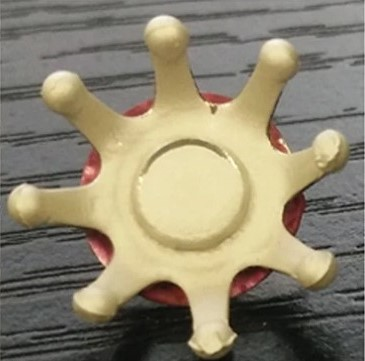
\includegraphics[height=4.2cm]{bilder/finger_electrodes.jpg}
    \quelle{\cite{xing2018}.}
    \caption{Fingerelektroden}
    \label{Fingerelektroden}
  \end{minipage}
  \hfill
  \begin{minipage}[t]{.47\linewidth}
    \centering
    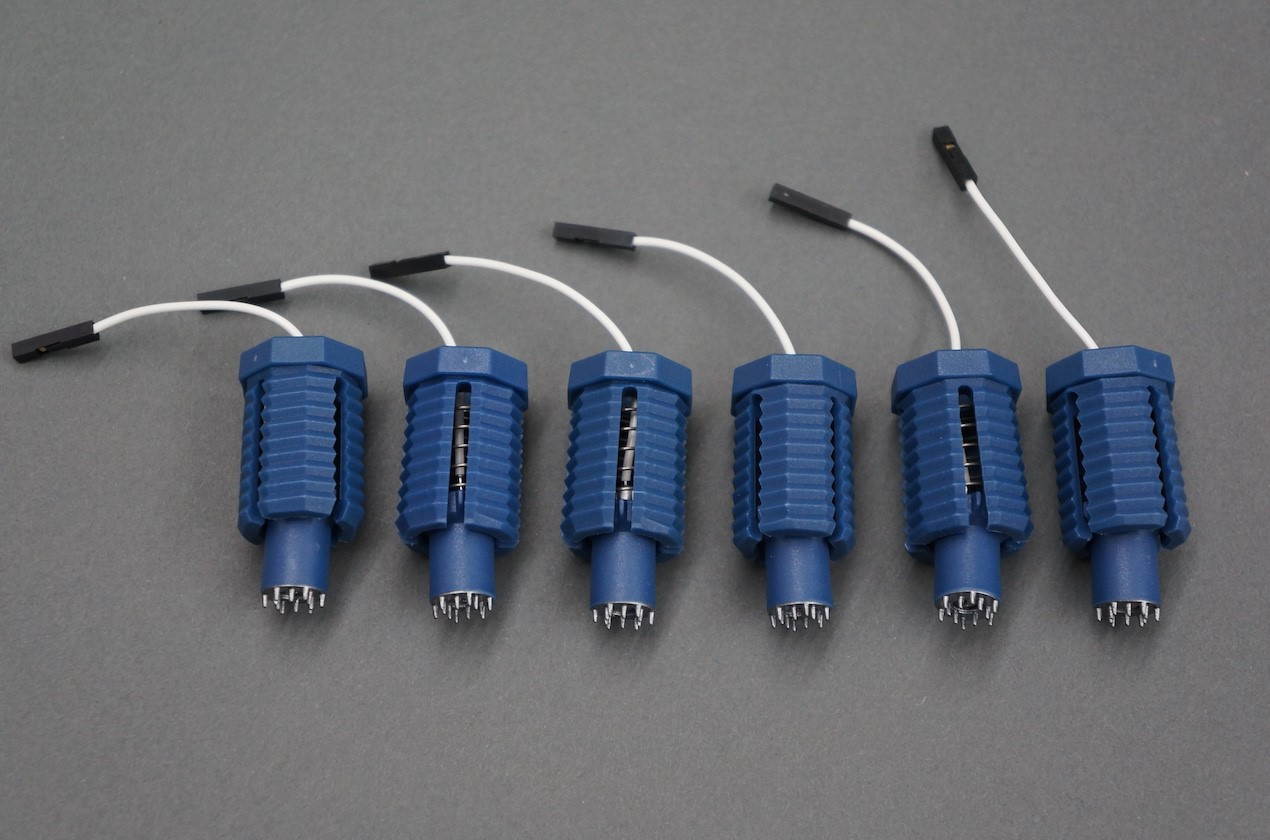
\includegraphics[height=4.2cm]{bilder/spikey_electrodes.jpg}
    \quelle{\cite{openbci_ultracortex_shop}.}
    \caption{Spitze Elektroden}
    \label{Spitze Elektroden}
  \end{minipage}
\end{figure}

Der Nachteil der Schwächung ist bei der Nutzung invasiver Elektroden (Abbildung \ref{invasiv}) nicht oder weniger vorhanden. Die raumzeitliche Auflösung ist höher, je näher die Elektroden den Neuronen, also den Quellen der Signale, sind. Das ermöglicht ein direktes Messen von Gehirnregionen und neuronalen Schaltkreisen. 
Die Nachteile sind das Risiko der chirurgischen Implantation, die fortgeschrittene und spezialisierte Herstellung, professionelle Operationen, die für die Messung durchgeführt werden müssen, höhere Kosten sowie dass ethische Gründe den Einsatz oft verhindern.\footnote{Vgl. \cite[S.~6]{qin2023}}

\begin{figure}[H]
	\centering
	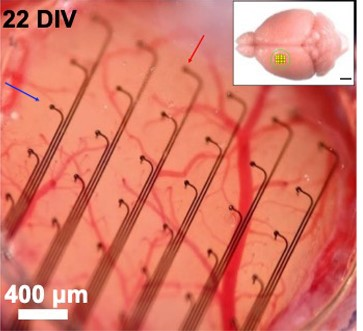
\includegraphics[width=0.4\textwidth]{bilder/invasive_electrode.jpg}
    \quelle{\cite{lee2022}.}
    \captionof{figure}{Beispiel für invasive Elektroden}
    \label{invasiv}
\end{figure}

Bei der Verwendung nicht-invasiver Elektroden gibt es verschiedene Möglichkeiten, diese anzuordnen. Die Formation ist abhängig von der Anzahl der Elektroden und der fokussierten Hirnregionen. Die besonders für nicht-invasive Elektroden standardisierte Elektrodenplatzierung ist das 10-20-System für 21 Elektroden, welches seit 1958 der Standard für klinische Messungen ist. Dabei sind die Messpunkte gleichmäßig verteilt. Viele Systeme arbeiten mit Kappen, an denen die Elektroden feste Plätze haben und nach dem 10-20-System angebracht werden. 10 und 20 stehen dabei für Prozentsätze: Benachbarte Elektroden liegen 10\,\% bzw. 20\,\% der Gesamtstrecke zwischen Nasion und Inion bzw. zwischen den beiden Ohren voneinander entfernt (Abbildung \ref{1020sys}). Weiterentwicklungen dieses Systems, wenn mehr Elektroden genutzt werden, werden 10-10- oder 10-5-System genannt. Die geringeren Abstände zwischen den Elektroden führen zu einer größeren Dichte von Elektroden und einer besseren räumlichen Auflösung.\footnote{Vgl. \cite{acharya2016_acns}}

\begin{figure}[H]
	\centering
	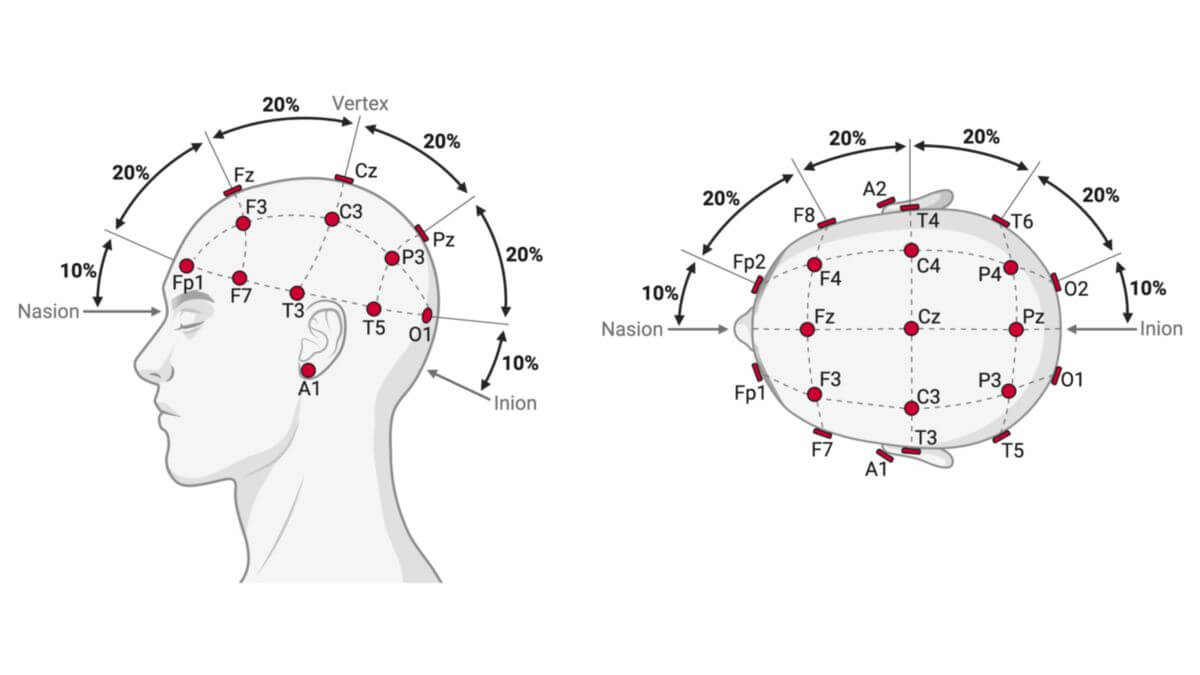
\includegraphics[width=0.75\textwidth]{bilder/1020_system.jpg}
    \quelle{\cite{doccheck_1020-system}.}
    \caption{Die Anordnung der Elektroden nach 10-20-System von der Seite und von oben betrachtet}
    \label{1020sys}
\end{figure}

Jede Elektrode wird mit einem Buchstaben und einer Ziffer kodiert (in manchen Fällen mit zwei Buchstaben). Die Buchstaben sind Abkürzungen für die darunterliegenden Lappen des Gehirns. Sie orientieren sich an den Gehörgangsöffnungen und an zwei festen Punkten, dem Nasion und Inion. Der Punkt Nasion ist in Abbildung \ref{nasion} markiert und der am weitesten vorne gelegene Punkt der Nahtstelle zwischen Stirnbein und dem linken und rechten Nasenbein. Die horizontale Ebene, auf der dieser Punkt liegt, trennt das Ober- vom Mittelgesicht.\footnote{Vgl. \cite{doccheck_nasion}} Der Punkt, der mit Inion bezeichnet wird, ist der am weitesten vorspringende Punkt des Os occipitale, eines platten Schädelknochens an der hinteren unteren Seite des Schädels, und in Abbildung \ref{inion} markiert.\footnote{Vgl. \cite{doccheck_inion}}

\begin{figure}[H]
  \centering
  \begin{minipage}[t]{.47\linewidth}
    \centering
    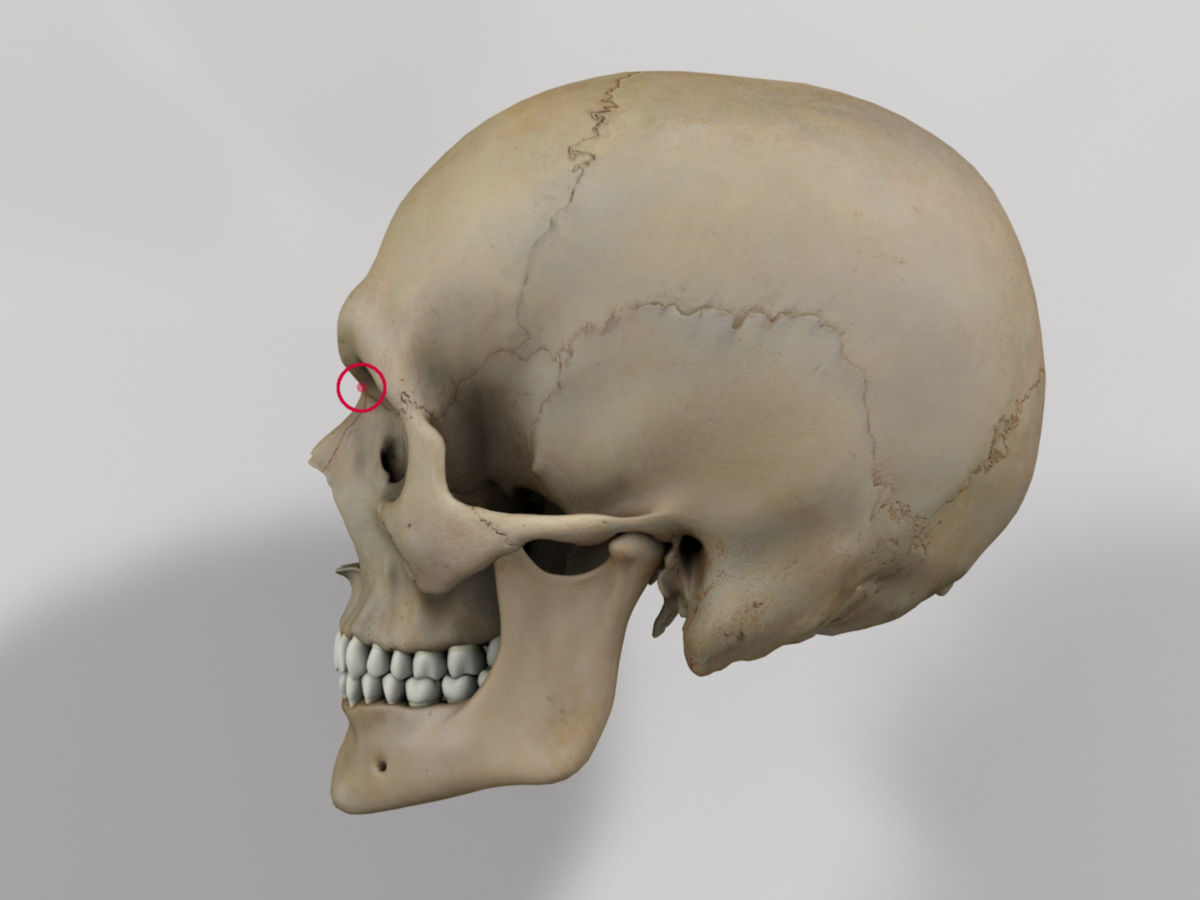
\includegraphics[height=5cm]{bilder/nasion.jpg}
    \quelle{\cite{doccheck_nasion}.}
    \caption{Position des Nasions}
    \label{nasion}
  \end{minipage}
  \hfill
  \begin{minipage}[t]{.47\linewidth}
    \centering
    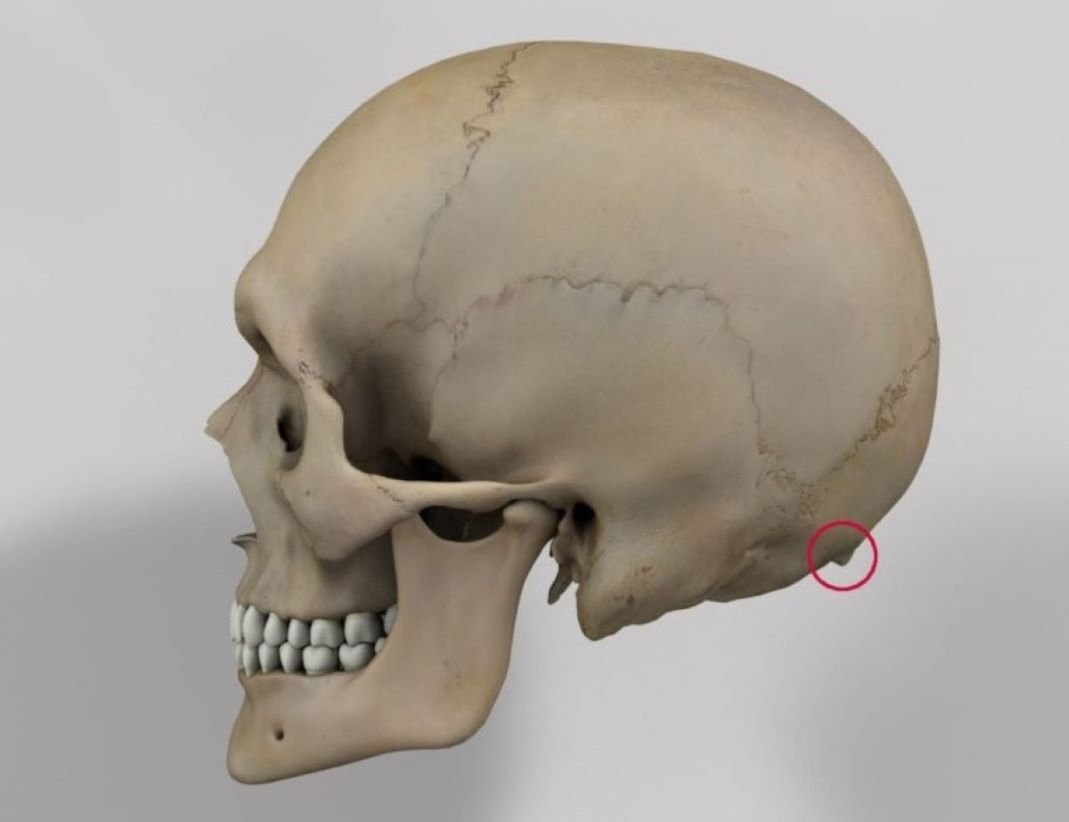
\includegraphics[height=5cm]{bilder/inion.jpg}
    \quelle{\cite{doccheck_inion}.}
    \caption{Position des Inions}
    \label{inion}
  \end{minipage}
\end{figure}

Die Buchstaben stehen für:
\begin{itemize}

    \item Fp = präfrontal - über präfrontalen Cortex
    \item F = frontal - über Frontallappen
    \item C = central - auf Verbindungslinie zwischen Gehörgangsöffnungen, in der Mitte der sagittalen (Nasion zu Inion) Linie
    \item T = temporal - über Temporallappen
    \item P = parietal - über Parietallappen
    \item O = okzipital - über Okzipitallappen
    \item A = aurikulär - am Ohr
    \item Z = zero (null) - ersetzt die Zahl an Elektroden zwischen Nasion und Inion, in der Mitte der koronaren (linke zu rechte Gehörgangsöffnung) Linie\footnote{Vgl. \cite{martinclemente2018}}

\end{itemize}
Elektroden, die auf der rechten Seite des Kopfes (rechts der sagittalen Linie) anliegen, werden mit einer geraden Nummer kodiert, links liegende mit einer ungeraden Nummer. Alle Zahlen nehmen von zentral zu temporal zu.\footnote{Vgl. \cite{doccheck_1020-system}}

Mit Z bezeichnete Elektroden werden oft als Referenzelektroden genutzt, da sie keiner Gehirnhälfte angehören. Hirnaktivität zeichnen allerdings auch sie auf.
Referenzelektroden spielen bei der Messung und im nächsten Schritt eine Rolle: der Vorverarbeitung. Diese geschieht durch Filter, Verstärker und die Ground- und Referenzelektroden.
Die Filter eliminieren ungewollte Störungen, behalten jedoch die Hauptfrequenz bei. Verstärker werden eingesetzt, um die geringen Amplituden des Signals (das Rohsignal liegt im Mikrovoltbereich) zu erhöhen (zum Beispiel in den Millivoltbereich), dadurch wird es einfacher, sie digital aufzuzeichnen.\footnote{Vgl. \cite[S.~8]{qin2023}} Referenzelektroden sind an Stellen des Kopfes angebracht, an denen möglichst wenig Gehirnaktivität zu messen ist, und machen einen Spannungsvergleich mit den anderen Elektroden möglich. Die Groundelektrode an Stirn oder Wange misst nicht nur sehr wenig Hirnaktivität, sondern schafft ein gemeinsames elektrisches Bezugspotenzial für das Messsystem. Wenn sich elektromagnetische Felder in der Umgebung befinden, beispielsweise aufgrund eines Monitors, der neben der Messanordnung steht, misst die Groundelektrode die dadurch entstandene Spannung. Dies ist Problematisch und wirkt sich negativ auf die Datenqualität aus. Das Zusammenspiel beider Elektroden, Referenz und Ground, ermöglicht Berechnungen in der Vorverarbeitungsschaltung. Die von dort weitergegebenen Daten zeigen dadurch weitgehend nur noch die Aktivität des Gehirns.\footnote{Vgl. \cite{biopac_reference_ground}}

Anschließend werden analoge Spannungssignale in digitale Form umgewandelt. Dies geschieht im \acrshort{adc}. Die Daten werden an Prozessoren gesendet, die Echtzeit-Verarbeitung und Analyse von Rohdaten ermöglichen. Sie erstellen die Grundlage für nachfolgende Datenverarbeitung am Computer.
Dort werden die Signale nach Mustern durchsucht. Aus den erkannten und klassifizierten Mustern werden Schlüsse gezogen und, je nach Versuchsaufbau und Anwendungsbereich, Feedback gegeben.\footnote{Vgl. \cite[S.~7]{qin2023}}

\section{Auswertung von EEG-Daten: Frequenzbandanalyse und ereigniskorrelierte Potenziale}
\autor{Sophie Kleppe}

\subsection{Zwei verschiedene Perspektiven der EEG-Analyse}
\label{sec:perspektiven}

Um \acrshort{eeg}-Daten zu verstehen und zu interpretieren, können die Signale in zwei sich ergänzende Perspektiven unterteilt werden.\footnote{Vgl. \cite{biasiucci2019}}

Es wird erstens zwischen spontanen \acrshort{eeg}-Rhythmen unterschieden, die durch kontinuierliche elektrische Aktivität (in Form von Wellen) in unterschiedlichen Frequenzbereichen gekennzeichnet sind, und zweitens \acrshortpl{erp}, welche als zeitlich gebundene Spannungsänderungen in Reaktion auf bestimmte Ereignisse oder \glspl{stimulus} erscheinen.\footnote{Vgl. \cite{biasiucci2019,sur2009}} Beide Perspektiven unterscheiden sich also grundlegend in ihrer zeitlichen Struktur: Während \acrshort{eeg}-Rhythmen kontinuierlich und ereignisunabhängig sind, sind \acrshortpl{erp} kurzzeitig, gebunden an ein konkretes Ereignis und in der Regel erst durch Mittelung vieler Wiederholungen im Experiment erkennbar.\footnote{Vgl. \cite{biasiucci2019}}

Genau diese eben beschriebenen Perspektiven bilden die methodische Grundlage für die im Rahmen unserer Arbeit durchgeführte \gls{validierungsstudie}. Um die Validität der Daten des portablen \acrshort{eeg}-Systems zu bewerten, müssen deshalb beide Betrachtungsweisen bedacht werden. Aus diesem Grund wird zum einen die \gls{alphapower} stellvertretend für die spontanen Rhythmen herangezogen, zum anderen die P1-Komponente stellvertretend für die ereigniskorrelierten Potenziale.

Im Folgenden werden deshalb zunächst die Frequenzbandbereiche  und anschließend die \acrshortpl{erp}  erläutert, wobei ein besonderer Fokus auf die in unserer Studie gewählten Vergleichsgrößen gelegt wird. Ausführlichere Beschreibungen weiterer Bänder und Komponenten finden sich im Anhang. Abschließend werden auch allgemeine Störgrößen behandelt, die später bei der Verarbeitung der in der Studie aufgenommenen Rohdaten beachtet werden müssen. 

\subsection{EEG-Rhythmen in verschiedenen Frequenzbandbereichen - Frequenzbandanalyse}

\acrshort{eeg}-Signale enthalten rhythmische Oszillationen, welche historisch in verschiedene Frequenzbänder unterteilt wurden, die mit griechischen Buchstaben bezeichnet werden. Diese inkludieren Delta ($\delta$)-, Theta ($\theta$)-, Alpha ($\alpha$)-, Beta ($\beta$)- und Gamma ($\gamma$)-Bänder sowie spezielle Bänder wie $\mu$ und $\sigma$.\footnote{Vgl. \cite{nayak_waveforms}} Jedes Band wird mit bestimmten Gehirnzuständen oder Funktionen assoziiert. Die Frequenzbänder werden mit einer \gls{spektralanalyse} aus dem \acrshort{eeg}-Signal bestimmt.\footnote{Vgl. \cite{biasiucci2019}}

Unter einem Frequenzband wird dabei ein definierter Frequenzbereich verstanden, in dem charakteristische \acrshort{eeg}-Aktivität auftritt. Die elektrische Aktivität selbst beschreibt die im \acrshort{eeg} gemessenen Signale, während regelmäßig auftretende, strukturierte Muster, zum Beispiel in Wellen ähnlicher Frequenz und Amplitude, dieser Aktivität als Rhythmen bezeichnet werden.

Die verschiedenen Frequenzbänder unterscheiden sich dabei aber nicht ausschließlich durch ihre Frequenz, auch die Amplitude, die \gls{topographie} und der assoziierte mentale und physiologische Zustand sind unterschiedlich. Tabelle~\ref{tab:frequenzbaender} stellt die verschiedenen Frequenzbänder anhand ihrer Unterscheidungsmerkmale gegenüber.

\begin{table}[htbp]
\centering
\caption{Übersicht der physiologischen EEG-Frequenzbänder und ihrer Eigenschaften}
\label{tab:frequenzbaender}
\begin{tabular}{ll p{7.5cm}}
\toprule
\textbf{Band} & \textbf{Frequenz (Hz)} & \textbf{Physiologischer Zustand} \\
\midrule
Delta ($\boldsymbol{\delta}$) & 0,5 -- 4   & Tiefschlaf \\
Theta ($\boldsymbol{\theta}$) & 4 -- 7     & Schläfrigkeit, frühe Schlafstadien \\
Alpha ($\boldsymbol{\alpha}$) & 8 -- 12    & Wacher, entspannter Zustand mit geschlossenen Augen \\
Beta ($\boldsymbol{\beta}$)   & 13 -- 30   & Wachzustand; Bewegungssteuerung und Aufmerksamkeit \\
Gamma ($\boldsymbol{\gamma}$) & $> 30$     & Sensorische und kognitive Verarbeitung \\
\bottomrule
\end{tabular}
\tabquelle{Eigene Darstellung nach \cite{nayak_waveforms}}
\end{table}
Wird die Topographie betrachtet, zeigt sich, dass Delta, Theta und Beta vermehrt frontozentral auftreten und Gamma über viele Hirnregionen verteilt ist, während Alpha \gls{posterior} und okzipital-dominant ist.\footnote{Vgl. \cite{nayak_waveforms}}
Werden die assoziierten mentalen und physiologischen Zustände betrachtet, lässt sich feststellen, dass niedrige Frequenzen wie Delta-Wellen vor allem in tiefen Schlafphasen dominieren, während höhere Frequenzen wie Beta- und Gamma-Wellen mit aktiver kognitiver Verarbeitung und Aufmerksamkeit assoziiert sind.\footnote{Vgl. \cite{nayak_waveforms}} Es ist jedoch zu beachten, dass diese Zuordnungen keine eindeutigen Zustände darstellen, da im Gehirn meist mehrere Frequenzbereiche gleichzeitig aktiv sind und sich überlagern.\footnote{Vgl. \cite{biasiucci2019}}

\subsection{Der Alpha-Rhythmus}
\label{sec:alpha}

Der Alpha-Rhythmus war die erste beschriebene, von Hans Berger entdeckte \acrshort{eeg}-Oszillation.\footnote{Vgl. \cite{jensen2010}} Im Wachzustand tritt Alpha insbesondere posterior über dem Okzipitallappen auf. Bei geschlossenen Augen oder geistiger Entspannung ist die Amplitude am höchsten, während sie sich bei geöffneten Augen oder geistiger Anstrengung deutlich verringert. Diese Abschwächung wird als \gls{berger-effekt} bezeichnet.\footnote{Vgl. \cite{nayak_waveforms}}

Die korrekte Abbildung des Alpha-Rhythmus eignet sich besonders gut als Kriterium, um zwei \acrshort{eeg}-Systeme miteinander zu vergleichen, da sein Auftreten durch den Berger-Effekt gut vorhersagbar ist.\footnote{Vgl. \cite{nayak_waveforms}} Zusätzlich ist dieses Phänomen gut untersucht\footnote{Vgl. \cite{barry2007}} und lässt sich leicht im folgenden beschriebenen Versuch einbauen (vgl. Kapitel~\ref{chap:methodik}).

\subsection{Bedeutung und Anwendungen der Frequenzbänder in BCI-Systemen}
\label{sec:bcibaender}

In der Klinik ist die Grundlage der \acrshort{eeg}-Auswertung die Kenntnis der normalen \acrshort{eeg}-Rhythmen und deren Abgrenzung zu abnormalen, krankhaften Mustern, wie etwa bei Epilepsie oder Hirnschädigungen.\footnote{Vgl. \cite{nayak_waveforms}} Die Analyse von Frequenzbändern hat jedoch auch großes Potenzial zur Nutzung in \acrshort{bci}-Anwendungen. Grund dafür ist insbesondere die Möglichkeit der gezielten Modulation \glsdisp{smr}{sensomotorischer Rhythmen}. Das bedeutet, dass die Stärke dieser Rhythmen durch die Person selbst beeinflussbar ist. Dafür ist allerdings häufig ein Training mittels \gls{neurofeedback} notwendig. Ist dieses erfolgt, kann die veränderte Rhythmusstärke in einen Befehl umgewandelt werden. Anwendungsziele liegen insbesondere in der Steuerung von \glspl{neuroprothese} durch gelähmte Menschen.\footnote{Vgl. \cite{wolpaw2002}} Bereits gelungen ist die Steuerung eines Cursors auf einem Bildschirm in x- und y-Richtung über die $\mu$- und Beta-Aktivität.\footnote{Vgl. \cite{wolpaw2004}} Versuchspersonen waren gesunde Menschen sowie Menschen mit Verletzungen des Rückenmarks. Dies stellt einen zentralen Durchbruch in der \acrshort{bci}-Forschung dar, da bis dahin angenommen wurde, dass dies nur über kortikal implantierte Elektroden möglich sei.\footnote{Vgl. \cite{wolpaw2004}} Auch gelungen ist das Greifen eines Gegenstands mit der gelähmten Hand einer Versuchsperson durch das Vorstellen einer Fußbewegung (Motor Imagery), was kurze, deutliche Ausbrüche von Beta-Aktivität zur Folge hatte (zur Funktionsweise vgl. Anhang, Abschnitt \glqq Steuerung einer Neuroprothese über Beta-Aktivität\grqq{}).\footnote{Vgl. \cite{pfurtscheller2003}} Gemeinsame Voraussetzung aller Beispiele ist allerdings das zuverlässige Erfassen dieser Rhythmen durch das verwendete \acrshort{eeg}-System. In diesen Studien kamen stationäre Forschungs- bzw. Laborsysteme zum Einsatz. 

\subsection{Ereigniskorrelierte Potenziale (ERPs)}
\label{sec:erp}

\subsubsection{Grundprinzip und Abgrenzung zu spontanen Rhythmen}

Während \acrshort{eeg}-Rhythmen den generellen Zustand des Gehirns widerspiegeln, sind \acrshortpl{erp} neuronale Reaktionen, welche mit bestimmten sensorischen, kognitiven oder motorischen Ereignissen verbunden sind und aus dem gesamten \acrshort{eeg} extrahiert werden können.\footnote{Vgl. \cite[S.~4]{luck2005}} Da jede dieser ereignisausgelösten neuronalen Reaktionen klein im Vergleich zur Gesamtheit aller gleichzeitig registrierten \acrshort{eeg}-Signale ist, werden in den meisten \acrshort{eeg}-Experimenten \acrshort{erp}-Wellen durch verschiedene Signalmittelungen von zufälligem Hintergrundrauschen isoliert.\footnote{Vgl. \cite[S.~56]{luck2005}}

\subsubsection{Abgrenzung der ERP-Komponenten voneinander}
\acrshort{erp}-Kurven bestehen aus einer Serie positiver und negativer Spannungsausschläge, wobei die einzelnen Ausschläge die verschiedenen Komponenten darstellen (vgl. Abbildung~\ref{fig:erp_schema}).\footnote{Vgl. \cite{biasiucci2019}} Die Benennung der Komponenten erfolgt folgendermaßen: Zunächst wird die Polarität relativ zur \gls{baseline_erp} (mittlere Spannung im Zeitraum unmittelbar vor dem Reiz) bestimmt. Positive Ausschläge werden dabei mit einem P gekennzeichnet, negative mit N. Darauf folgt entweder der Zeitpunkt des Ausschlags (Latenz) (z.\,B. \gls{p300} = positiver Ausschlag bei 300\,ms) oder die Reihenfolge, in der die Komponente auftritt (P1 = erster positiver Ausschlag). Eine Ausnahme bildet die C1-Komponente, deren Polarität je nach Ort der Präsentation des Stimulus im Gesichtsfeld (unteres Gesichtsfeld = positiv, oberes Gesichtsfeld = negativ) variieren kann.\footnote{Vgl. \cite[S.~35]{luck2005}} Was verwendet wird, hängt davon ab, wie stark die Latenz schwankt und ob sich die Ausschläge besonders bei späten Komponenten klar trennen lassen.\footnote{Vgl. \cite[S.~35--43]{luck2005}} Tabelle~\ref{tab:erp} soll einen Überblick über die Unterscheidungsmerkmale wie Latenz und Topographie der vier frühen visuellen \acrshort{erp}-Komponenten geben.

\begin{table}[htbp]
\centering
\caption{Unterscheidungsmerkmale der frühen visuellen ERP-Komponenten C1, P1, N1 und P2}
\label{tab:erp}
\small
\begin{tabularx}{\textwidth}{@{}l l >{\raggedright}p{3.1cm} >{\raggedright}p{3.3cm} >{\raggedright\arraybackslash}X@{}}
\toprule
\textbf{Komp.} & \textbf{Polarität} & \textbf{Latenzfenster} & \textbf{Topographie} & \textbf{Ursprung / Funktion / Sensitivität} \\
\midrule
C1 & Variabel & Onset: $\approx$ 40--60 ms \newline Peak: $\approx$ 80--100 ms & Posteriore Mittellinie & Primäre Sehrinde (V1), sensitiv für physikalische Reizmerkmale \\
\addlinespace
P1 & Positiv  & Onset: $\approx$ 60--90 ms \newline Peak: $\approx$ 100--130 ms & \Gls{lateral} okzipital & Frühe visuelle Verarbeitung, sensitiv für Kontrast \& Größe \\
\addlinespace
N1 & Negativ  & $\approx$ 100--200 ms \newline (Mehrere Subkomponenten) & \Gls{anterior} (früh), parietal \newline \& lateral okzipital (spät) & Aufmerksamkeitsbezogene Reizverarbeitung \\
\addlinespace
P2 & Positiv  & $\approx$ 150--250 ms & Anterior-zentral & Höhere visuelle Analyse, oft überlappt durch N1/N2 \\
\bottomrule
\end{tabularx}
\tabquelle{Eigene Darstellung nach \cite[S.~35--43]{luck2005}; \cite{dirusso2002}}
\end{table}

Insgesamt zeigt sich, dass die Komponenten in der zeitlichen Abfolge C1, P1, N1 und P2 innerhalb eines Zeitfensters von 40--250 ms nach dem auslösenden Ereignis auftreten. Je später die Latenz, desto schwerer ist auch die Isolation der Komponenten, da sich die elektrischen Signale im Gehirn zunehmend überlappen.\footnote{Vgl. \cite[S.~35]{luck2005}}

\begin{figure}[H]
\centering
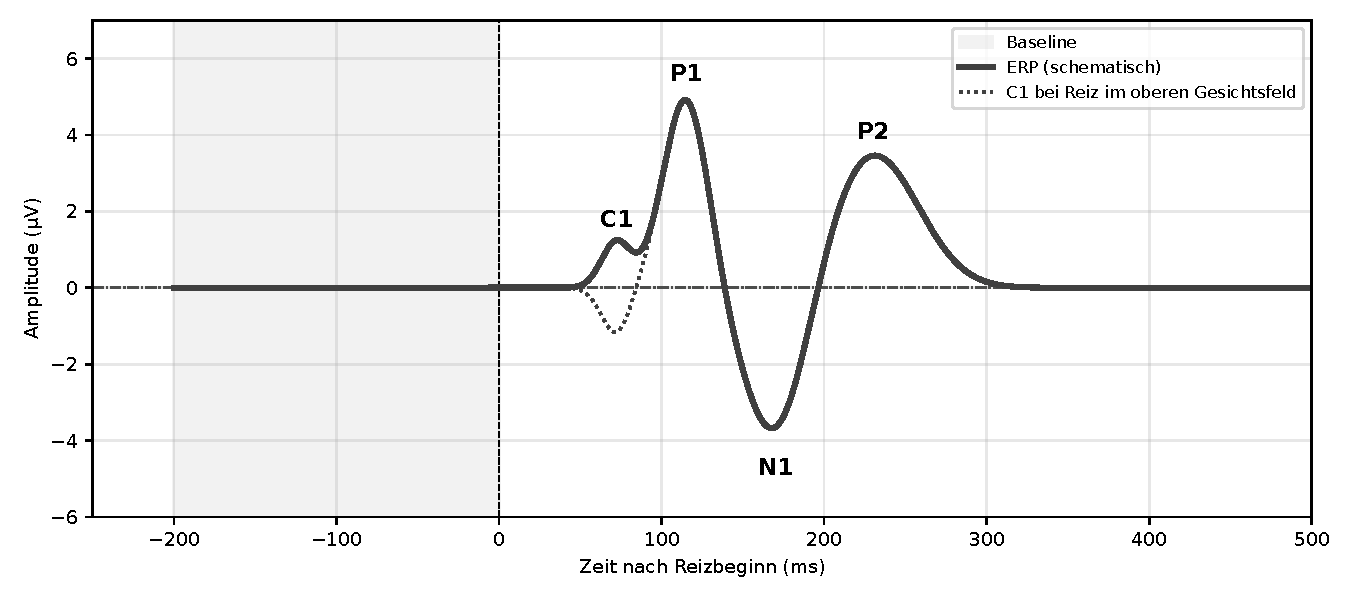
\includegraphics[width=0.85\textwidth]{bilder/erp_schema.pdf}
\quelle{Eigene Darstellung nach \cite{luck2005} und \cite{dirusso2002}.}
\caption{Schematischer Verlauf eines visuellen ereigniskorrelierten Potenzials mit den frühen Komponenten C1, P1, N1 und P2}
\label{fig:erp_schema}
\end{figure}

Im nächsten Abschnitt werden vor allen Dingen die charakteristischen Merkmale der P1-Komponente betrachtet, da diese Komponente als weiteres Vergleichskriterium dieser Validierungsstudie dient. Alle weiteren ausführlichen Beschreibungen der anderen Komponenten finden sich im Anhang.

\subsubsection{Die P1-Komponente}

Die positive P1-Komponente erreicht an den lateral okzipitalen Elektroden ihre maximale Amplitude, tritt 60--90 ms nach dem Reiz auf und erreicht ihr Maximum bei 100--130 ms. Sie ist allerdings schwierig genau zu identifizieren, da sie sich mit der C1-Welle überlappt. Die P1-Latenz und -Amplitude können sich maßgeblich durch den Stimuluskontrast verändern.\footnote{Vgl. \cite[S.~36]{luck2005}}

Genau diese Eigenschaften der P1 sind ausschlaggebend für die Eignung als Validierungskriterium für unsere Studie: Erstens kann die Auswertung hauptsächlich auf die lateral okzipitalen Elektroden beschränkt werden, da die P1 ihre maximale Amplitude an diesen Elektroden erreicht, und zweitens lässt sich das Verhalten der P1 gegenüber Kontrast- und Größenabhängigkeit des Stimulus gut vorhersagen. Dies bedeutet in der Praxis, dass die P1, wenn Versuchspersonen ein großes und kontrastreiches Bild sehen, eine geringere Latenz und größere Amplitude aufweisen müsste, als wenn sie ein kleines Bild mit geringem Kontrast sehen. 

\subsection{Einflussfaktoren und Störgrößen}
\label{sec:stoer}

Um aufschlussreiche Ergebnisse aus der \acrshort{eeg}-Analyse zu gewinnen, müssen einige wichtige Aspekte berücksichtigt werden. \acrshort{eeg}-Signale sind von Natur aus schwach und sehr verrauscht, und viele technische und psychologische Faktoren können die Messung beeinflussen. Im Folgenden werden einige Punkte aufgeführt, welche bei \acrshort{eeg}-Experimenten beachtet werden müssen.

\textbf{Artefakte und Rauschen:} \acrshort{eeg}-Aufzeichnungen sind grundsätzlich mit Artefakten kontaminiert. Artefakte sind Signale, welche nicht von der Gehirnaktivität stammen.\footnote{Vgl. \cite{jiang2019}} Häufige Artefakte umfassen Augenblinzeln und Augenbewegungen (diese produzieren große Spannungsabweichungen durch das Stehpotenzial des Auges), Muskelaktivität (Gesichts- und Nackenmuskeln können hochfrequente Störgeräusche verursachen), Herzsignale (der Puls kann rhythmische Störungen verursachen) und externe elektrische Störungen (Netzstromstörungen bei 50/60 Hz) sowie Schweißbildung auf der Kopfhaut (Elektrolyte im Schweiß können die Leitfähigkeit verändern und dadurch langsame Signalverschiebungen oder Drift verursachen).\footnote{Vgl. \cite{jiang2019}; \cite{muthukumaraswamy2013}; \cite{light2010}; \cite{kappenman2010}} 

Da einige Artefakte echte Gehirnströme imitieren oder verdecken können (z.\,B. können Verspannungen der Kopfhautmuskulatur Frequenzen von etwa 20\,Hz bis über 100\,Hz erzeugen, welche fälschlicherweise als Beta oder Gamma interpretiert werden könnten), ist ein sorgfältiger Umgang mit Artefakten entscheidend.\footnote{Vgl. \cite{muthukumaraswamy2013}} Dies kann vorbeugende Maßnahmen (z.\,B. Hinweise an die Versuchsperson, Bewegungen zu minimieren) sowie Nachbearbeitungsmethoden umfassen.\footnote{Vgl. \cite{light2010}} Eine Möglichkeit ist beispielsweise die Filterung (z.\,B. Verwendung eines \gls{notch} bei 50 Hz, um Netzrauschen zu entfernen). Dabei wird zwischen zwei Arten von Störungen unterschieden: äußeren Störungen, wie z.\,B. Netzbrummen bei 50\,Hz, welche meist durch einfache Filtermethoden entfernbar sind, sowie Störungen, welche vom Körper ausgehen und häufig im selben Frequenzbereich wie die eigentlichen vom \acrshort{eeg} aufgezeichneten Daten liegen und somit nicht durch Filtermethoden entfernt werden können, da sonst auch die Hirnaktivität verloren gehen würde.\footnote{Vgl. \cite{jiang2019}} Ein Beispiel dafür ist die Aktivität der Kiefermuskeln, welche vollständig mit dem Gamma-Band überlappt.\footnote{Vgl. \cite{muthukumaraswamy2013}}

Aufgrund dessen sind gesonderte Verfahrensweisen notwendig. Dazu zählt die Regression: Bei diesem Verfahren wird das Artefakt, beispielsweise Augenbewegungen, über eigene Elektroden an den Augen (Elektrookulographie, \acrshort{eog}) separat gemessen. Anschließend wird berechnet, wie stark sich dieses Artefakt auf jede \acrshort{eeg}-Elektrode auswirkt, und dieser Anteil wird abgezogen. Ein weiteres Verfahren ist die Unabhängigkeitskomponentenanalyse (\acrshort{ica}), mittels der das Signal in unabhängige Signalquellen (sogenannte \acrshort{ica}-Komponenten) zerlegt wird und anschließend Artefakte wie z.\,B. Lidschläge entfernt werden (vgl. Abschnitt~\ref{sec:p1auswertung}). Heute wird hauptsächlich die \acrshort{ica} genutzt, da kein zusätzlicher Kanal notwendig ist und auch Artefakte, welche nicht durch einen eigenen Kanal erfasst werden können, entfernt werden können.\footnote{Vgl. \cite{jiang2019}} Bei der Validierung eines \acrshort{eeg}-Geräts muss geprüft werden, dass das System eine ausreichende Signalqualität mit wenig Rauschen aufweist, sodass Artefakte zuverlässig entfernt werden können und die zu messenden Gehirnströme nicht in Verstärkerrauschen oder Interferenz untergehen.

\textbf{Elektrodenanordnung und Referenz:} Da \acrshort{eeg}-Messungen Spannungsunterschiede messen, hat die Wahl einer Referenzelektrode signifikanten Einfluss auf die aufgezeichneten Wellen. Das liegt daran, dass es keinen neutralen Punkt am Körper gibt (das sogenannte \gls{no-switzerland-principle}), sodass jede Referenzwahl (egal ob am Ohrläppchen, Mastoid (Teil des Schläfenbeins hinter dem Ohr), Vertex Cz oder einem Durchschnitt aller Elektroden) einen gewissen \gls{bias} oder ein Profil auf den Daten hinterlässt.\footnote{Vgl. \cite{yao2019}; \cite{biasiucci2019}} Viele moderne \acrshort{eeg}-Systeme erlauben es, später die Referenz zu ändern (z.\,B. zur \gls{durchschnittsreferenz}).\footnote{Vgl. \cite{yao2019}} Das nachträgliche Ändern ist insbesondere notwendig, wenn zwei zu vergleichende Systeme mit unterschiedlichen Referenzen messen, da diese die Ergebnisse erheblich verändern (vgl. Abschnitt~\ref{sec:vorverarbeitung}). Ebenfalls ist die standardisierte Elektrodenanordnung (internationales 10-20-System) wichtig, um sicherzustellen, dass bekannte Muster in den korrespondierenden Kanälen angezeigt werden.\footnote{Vgl. \cite{acns_guideline2}}

\textbf{Filter und Signalbandbreite:} \acrshort{eeg}-Signale umfassen ein breites Spektrum an Frequenzen, von langsamen Gleichspannungsanteilen (< 0,5 Hz) bis zu 100 Hz oder mehr.\footnote{Vgl. \cite{nayak_waveforms}} Um sich auf die relevanten Frequenzbänder zu fokussieren und Rauschen zu reduzieren, werden normalerweise \glspl{bandpass} angewendet, welche nur Signale zwischen einer unteren und einer oberen \gls{cutoff} passieren lassen. Gängige Bandpässe für Aufzeichnungen von \acrshortpl{eeg} bei Erwachsenen reichen beispielsweise von etwa 0,01--0,5\,Hz (\gls{hochpass}) bis 100\,Hz (\gls{tiefpass}), wodurch der herkömmliche Delta- bis Gammabereich erhalten bleibt und hochfrequente Störgeräusche sowie langsame Verschiebungen herausgefiltert werden.\footnote{Vgl. \cite{light2010}; \cite{wikipedia_eeg_highpass}} Es ist von essenzieller Bedeutung, vor der Analyse geeignete Filtereinstellungen zu wählen. So kann beispielsweise ein zu hoher Hochpassfilter langsame Wellen und \acrshortpl{erp} verzerren, während ein zu niedriger Tiefpassfilter auch gewünschte schnelle Aktivität entfernen kann.\footnote{Vgl. \cite{wikipedia_eeg_highpass}} Tatsächlich haben Forscher herausgefunden, dass bereits eine Hochpassgrenzfrequenz von etwa 0,3\,Hz die scheinbare Amplitude der \gls{p300} deutlich reduzieren kann, was unterstreicht, wie sich die Wahl des Filters auf die gemessenen Signale auswirkt.\footnote{Vgl. \cite{holinger2000}}

\textbf{Subjektfaktoren und Versuchsaufbau:} \acrshort{eeg}-Systeme reagieren sehr empfindlich auf den Zustand der Versuchsperson und den Versuchsaufbau. Vor der Analyse der Daten müssen Faktoren wie der Wachheitsgrad, die Müdigkeit und die Bewegungen der Versuchsperson sowie Faktoren wie Raumgeräusche oder Änderungen der Elektrodenimpedanz betrachtet werden.\footnote{Vgl. \cite{kappenman2010}} Viele dieser Faktoren können die Ergebnisse beeinflussen oder verfälschen: So weist beispielsweise eine schläfrige Versuchsperson mehr Theta-Wellen auf und kann somit die \gls{baseline_alpha} der \qt{Alpha-/Betaleistung} verzerren.\footnote{Vgl. \cite{nayak_waveforms}} Ein weiteres Beispiel ist, wenn die Versuchspersonen sich während der Aufzeichnung langweilen, wodurch überdurchschnittlich viel Alpha produziert wird. Daher ist es wichtig, den Zustand der Versuchsperson zu kontrollieren oder zu überwachen (manche Protokolle quantifizieren sogar Augenblinzeln oder inkludieren \acrshort{eog}-Kanäle, um die Wachsamkeit zu berücksichtigen).\footnote{Vgl. \cite{nayak_waveforms}} Für \acrshortpl{erp} muss das experimentelle \gls{paradigma} gut designt sein. Stimuli sollten mit präzisem Timing präsentiert werden (oft unter Verwendung von \glspl{eventmarker}) und der Versuch mit hinreichender Wiederholung durchgeführt werden, um eine Durchschnittsbildung zu ermöglichen.\footnote{Vgl. \cite{light2010}}

Genau diese Störgrößen bilden die Grundlage für die Vorverarbeitung (z.\,B. durch Bandpassfilterung, Anwendung eines \gls{notch}s, Re-Referenzierung und die Interpolation defekter Elektroden) der in unserer Studie gewonnenen Daten. 

\section{Merkmale von Brain-Computer-Interfaces und mögliche Anwendungen}
\label{sec:bci}
\autor{Alisa Fiedler}

Die zuvor beschriebene Frequenzbandanalyse ist eine wichtige Grundlage für die Funktionsweise von \acrshortpl{bci}.

Ein \acrshort{bci} ermöglicht \glqq eine direkte Informationsübertragung zwischen einem organischen Gehirn und einem technischen Schaltkreis\grqq{}.\footnote{\cite{heuer2015}}
Es nimmt neuronale Signale auf, analysiert und übersetzt diese in Befehle, ohne dass eine Muskelbewegung erforderlich ist.
Dadurch schaffen \acrshortpl{bci} völlig neue und kreative Möglichkeiten, Geräte zu steuern, die unabhängig von körperlicher Bewegung oder Sprache funktionieren.\footnote{Vgl. \cite{heuer2015}}

Die Funktionsweise eines \acrshort{bci} beruht auf der kontinuierlichen Erfassung physiologischer Signale, vor allem der elektrischen Aktivität des Gehirns.
Diese wird mithilfe eines \acrshort{eeg} gemessen.
Die Signale, die aufgezeichnet werden, werden mit vorab festgelegten oder erlernten Mustern verglichen, um charakteristische neuronale Signale festzustellen, die gleichzeitig als Kontrollsignale dienen.\footnote{Vgl. \cite{heuer2015}}
Durch die Analyse dieser Kontrollsignale kann das \acrshort{bci} die Intentionen des Benutzers erkennen und diese sodann in Steuerbefehle umsetzen.
Damit ein \acrshort{bci} zuverlässig funktioniert, müssen die Signale möglichst genau ausgewertet und in Echtzeit verarbeitet werden.
Gleichzeitig können äußere Störsignale sowie Unterschiede zwischen den Nutzern die Signalverarbeitung und Interpretation erschweren.
Dies führt dazu, dass die Interpretation der Signale anfällig für Fehler ist und nicht immer zwischen verschiedenen Gehirnaktivitätszuständen unterschieden werden kann.
In der Praxis erfordert dies daher eine ausführliche Signalverarbeitung sowie oft eine Anpassung des Systems an den jeweiligen Nutzer.\footnote{Vgl. \cite{wolpaw2002}}

Ein vereinfachtes Beispiel für ein \acrshort{bci}-System wurde im Rahmen eines Informatikprojekts in der 10. Klasse umgesetzt.
Dabei wurden \acrshort{eeg}-Daten von einem portablen \acrshort{eeg} in Echtzeit erfasst, analysiert und als Spiel visuell dargestellt.
Die Auswertung der \acrshort{eeg}-Daten basierte auf der Analyse des bestimmten Frequenzbereiches Alpha, die Rückschlüsse auf die mentale Aktivität des Nutzers ermöglichte.
Die Steuerung erfolgte über ein interaktives Spiel, bei welchem ein Ballon abhängig von der Gehirnaktivität gesteuert wurde. Dieses Projekt verdeutlichte die Funktionsweise eines \acrshort{bci}, da auch hier neuronale Signale verarbeitet und in eine visualisierte Auswertung der Gehirnströme überführt wurden.
Während in diesem Projekt nur eine visuelle Rückmeldung erzeugt wurde, lässt sich die gleiche Funktionsweise auf andere reale Systeme übertragen.
So können die analysierten Gehirnsignale auch genutzt werden, um einen Roboterarm, genannt Arduino Tinkerkit Braccio (vgl. Abbildung~\ref{roboter}), zu steuern.

\begin{figure}[H]
	\centering
    	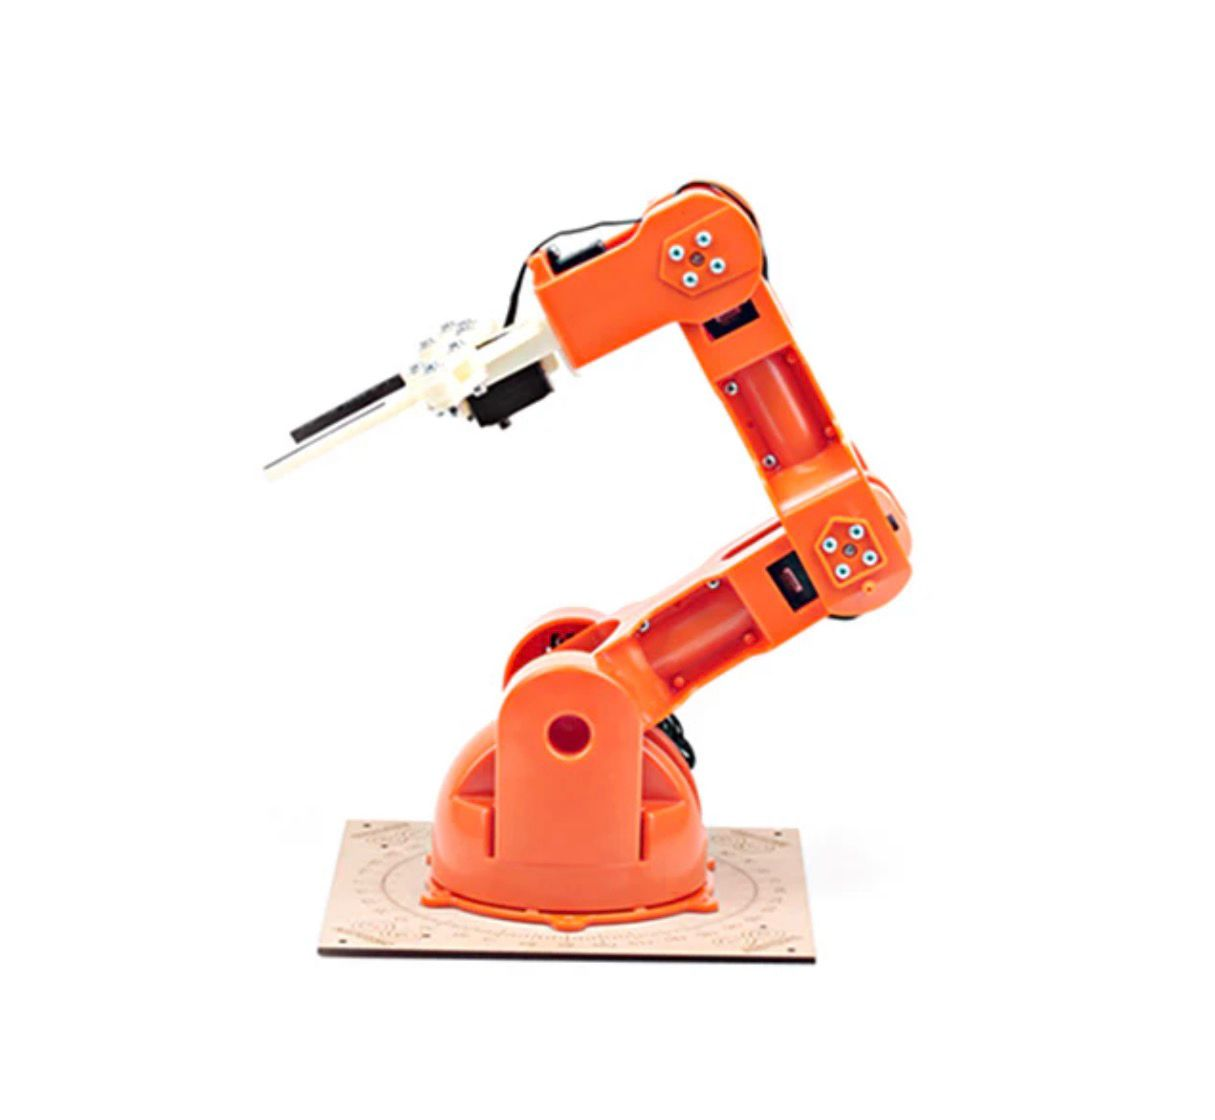
\includegraphics[width=0.5\textwidth]{bilder/roboter.jpeg}
    \quelle{\cite{arduino_braccio}.}
    \captionof{figure}{Roboterarm Arduino Tinkerkit Braccio}
    \label{roboter}
\end{figure}

Dabei werden die erkannten Muster nicht mehr nur abgebildet, sondern direkt in physische Bewegungen umgesetzt.
Im Rahmen der Seminarfacharbeit wird neben der Validierungsstudie eines portablen \acrshort{eeg}-Systems zusätzlich untersucht, ob die Daten des portablen Systems die Grundlage für die Steuerung eines Roboterarms mithilfe eines \acrshort{bci}-Programms bilden können.
Der Roboterarm ist dabei in der Lage, die durch das \acrshort{bci} erzeugten Signale zu verarbeiten und in gezielte Bewegungen umzusetzen.

\acrshortpl{bci} gewinnen in der heutigen Zeit an Bedeutung.
Insbesondere Menschen mit körperlichen Behinderungen können von der Technik mit der Umsetzung von \acrshortpl{bci} profitieren.
Es gibt bereits \glqq prototypische Systeme, die etwa die Steuerung eines Cursors, die Bedienung eines virtuellen Buchstabierprogramms oder die Kontrolle von robotischen bzw. prothetischen Effektoren erlauben\grqq{}.\footnote{\cite{heuer2015}}
Neben medizinischen Anwendungen gewinnen in den vergangenen Jahren auch nicht-medizinische Einsatzmöglichkeiten an Aufmerksamkeit.
Dazu zählen unter anderem die Steuerung von Fahrzeugen oder Robotern sowie die Überwachung von mentalen Zuständen.

\section{Fragestellung und Hypothesen}
\label{sec:fragestellung}
\autor{Sophie Kleppe}

Abschnitt~\ref{sec:bci} zeigt, dass Hirnaktivität in Steuerbefehle für \acrshort{bci}-Systeme übersetzt werden kann. Das ist vor allem für Menschen von Bedeutung, welche ihre Gliedmaßen nicht mehr gezielt bewegen können. Für Menschen mit Amputationen gibt es heute vielseitige Möglichkeiten, ihre Lebensqualität wiederherzustellen. Moderne Prothesen können über die Muskelsignale am Stumpf gesteuert werden, sodass eine sehr präzise Steuerung möglich ist. Querschnittsgelähmte haben dagegen zwar noch alle Extremitäten, können diese jedoch nicht mehr ansteuern, obwohl das Gehirn die Bewegung weiterhin planen kann. Für sie gibt es bisher nur wenige und eingeschränkte Möglichkeiten, wie z.\,B. \glspl{neuroprothese}, die die gelähmten Muskeln mithilfe elektrischer Impulse anregen und so etwa einen Griff ermöglichen. Diese benötigen allerdings ein Steuersignal. Bisher wird dieses aus Restbewegungen, bspw. der Schulter, gewonnen, die dem Patienten noch möglich sind. Bei einem hohen Lähmungsgrad sind diese Restbewegungen häufig aber auch nicht mehr vorhanden, weshalb an einer Steuerung mittels \acrshort{bci} geforscht wird.\footnote{Vgl. \cite{rupp2015}} Wie wichtig eine solche Steuerung wäre, zeigt eine Studie unter circa 680 Menschen mit Querschnittslähmung. Auffällig war, dass Menschen mit Tetraplegie, also einer Lähmung von Armen und Beinen, die Wiederherstellung der Arm- und Handfunktion als wichtigstes Ziel erachteten.\footnote{Vgl. \cite{anderson2004}} Dabei kann bereits eine einzige Greifbewegung ein Stück Selbstständigkeit zurückgeben. Eine solche \acrshort{bci}-Steuerung ist die langfristige Vision, an der diese Arbeit ansetzt. Ein Roboterarm kann dabei als vereinfachtes Modell dienen.

Neben dieser Vision ist die Arbeit auch für das DLR\_School\_Lab Jena von Bedeutung. Dort führen Schülerinnen und Schüler ab der 4.~Klasse unter Anleitung von Tutoren selbst Experimente zu aktuellen Forschungsthemen wie Robotik oder künstlicher Intelligenz durch.\footnote{Vgl. \cite{dlr_schoollab_jena}} Interessant ist hier die Frage, ob eine Experimentierstation aufgebaut werden könnte, an der Kinder und Jugendliche selbst erleben, wie ein \acrshort{bci} funktioniert, indem sie z.\,B. durch das Schließen der Augen eine Bewegung des Roboterarms auslösen. Im DLR\_School\_Lab gibt es jedoch keine abgeschirmte Kabine, und das Anlegen des Systems muss schnell gehen, um für eine Station geeignet zu sein.

Für beide Zielstellungen kommt ein günstiges und tragbares \acrshort{eeg}-System infrage. Es ermöglicht den Einsatz außerhalb eines Labors, welcher für eine Anwendung im Alltag nötig ist. Zudem ist es einfacher anzulegen, da die Elektroden trocken sind und somit ohne Gel auskommen.\footnote{Vgl. \cite{openbci_dry_electrodes}} Trotz der vielseitigen Vorteile gibt es auch entscheidende Nachteile, die im schlimmsten Fall eine Anwendung ausschließen könnten. Durch die Trockenelektroden kann es zu einem schlechteren Kontakt der Elektroden mit der Kopfhaut kommen, und im Alltag lassen sich Bewegungsartefakte nicht ganz vermeiden. Dies könnte dazu führen, dass Signale nicht mehr korrekt erfasst werden (vgl. Abschnitt~\ref{sec:stoer}).\footnote{Vgl. \cite{kappenman2010}} Bevor ein Roboterarm angesteuert werden kann, muss deshalb feststehen, dass das OpenBCI-System die Hirnaktivität zuverlässig aufzeichnet. Daher muss der erste Schritt zwingend eine Validierung durch den Vergleich mit einem stationären System als Referenz sein. Dafür wird das BioSemi-System genutzt, dieses steht im Institut für Psychologie in Jena. Dort wird mit Gelelektroden und aktiver Abschirmung, in Form eines Faradayschen Käfigs, gearbeitet.\footnote{Vgl. \cite{biosemi_active_electrodes}} Anschließend kann geklärt werden, ob das OpenBCI-System eine Grundlage für die spätere Initialisierung von Bewegungsabläufen des Roboterarms \glqq Arduino Tinkerkit Braccio\grqq{} bildet. Daraus ergibt sich die folgende Fragestellung.

\begin{quote}
\textit{Inwieweit lässt sich die Datenqualität des OpenBCI-Systems auch in einer alltagsnahen Umgebung mit der des BioSemi-Systems vergleichen, und genügt diese als Grundlage für das spätere Initialisieren von Bewegungsabläufen des Roboterarms?}
\end{quote}

Um die Fragestellung beantworten zu können, müssen zunächst Begriffe, die nicht direkt messbar sind, operationalisiert, das heißt in messbare Größen übersetzt, werden. Dazu muss für die zentralen Aspekte der Fragestellung geklärt werden, woran eine vergleichbare Datenqualität erkennbar ist, wie eine alltagsnahe Umgebung im Experiment umgesetzt werden kann und wann die Daten als Grundlage für die Steuerung des Roboterarms genügen.

\paragraph{Datenqualität} Die Datenqualität kann als vergleichbar angenommen werden, wenn sich bekannte Eigenschaften von \acrshort{eeg}-Signalen aus der Literatur in beiden Systemen klar erkennen lassen. Diese Eigenschaften müssen dabei beide Perspektiven der \acrshort{eeg}-Analyse abdecken, also sowohl spontane Rhythmen als auch \acrshortpl{erp} (vgl. Abschnitt~\ref{sec:perspektiven}). Daher werden der Alpha-Rhythmus und die P1-Komponente als Paradigmen herangezogen, deren Verhalten gut vorhersagbar ist (vgl. Abschnitte~\ref{sec:perspektiven}, \ref{sec:alpha} und~\ref{sec:erp}). Dadurch lässt sich vorab festlegen, welches Ergebnis ein System liefern muss, das die Hirnaktivität korrekt erfasst. Damit überprüfbar ist, wann diese Eigenschaften klar erkennbar sind, wird für jede ein Kriterium festgelegt.

Für das Alpha-Paradigma gelten die folgenden Kriterien:
\begin{itemize}
    \item Der Berger-Effekt muss nachweisbar sein, das heißt, das Verhältnis der Alpha-Power bei geschlossenen Augen (engl. eyes closed, \acrshort{ec}) zu geöffneten Augen (engl. eyes open, \acrshort{eo}), die sogenannte Alpha-Suppression, beträgt bei jeder Versuchsperson mindestens 2. Die Alpha-Power ist bei geschlossenen Augen also mindestens doppelt so hoch, damit ein Unterschied nicht allein durch zufällige Schwankungen erklärt werden kann.\footnote{Zum Anstieg der Alpha-Power bei geschlossenen Augen vgl. \cite{barry2007}}
    \item Die größte Alpha-Suppression liegt über den okzipital oder parietal liegenden Elektroden.
    \item Die Rangfolge der Versuchspersonen nach ihrer Alpha-Power stimmt zwischen den Versuchsbedingungen stark überein, das heißt, die \gls{spearman} beträgt mindestens 0,5.\footnote{Vgl. \cite{cohen1988}}
\end{itemize}

Für das P1-Paradigma gelten die folgenden Kriterien:
\begin{itemize}
    \item Die mittlere Amplitude der P1 ist für große, kontrastreiche Stimuli größer als für kleine, kontrastreduzierte Stimuli.\footnote{Vgl. \cite[S.~36]{luck2005}}
    \item Die P1 hebt sich vom Hintergrundrauschen ab, das \gls{snrgl} (\acrshort{snr}) ist also größer als 1.
\end{itemize}
Für beide Paradigmen wird zudem der Anteil der auswertbaren Datensätze je Versuchsbedingung angegeben und mit dem BioSemi-System verglichen. Wie diese Größen berechnet werden, ist in Abschnitt~\ref{sec:auswertung} beschrieben. Dabei ist nicht zu erwarten, dass beide Systeme identische Werte liefern, da sie sich in Elektroden und Verstärkern unterscheiden. Entscheidend ist, dass die genannten Kriterien erfüllt sind. Ist dies beim OpenBCI-System nicht der Fall, kann die Datenqualität nicht als vergleichbar angenommen werden.

\paragraph{Alltagsnahe Umgebung} Als alltagsnah gilt eine Umgebung, die eine Anwendung im DLR\_School\_Lab und im Alltag ermöglicht, also ohne Kinnstütze und ohne vollständig abgeschirmte Kabine. Um dies umzusetzen, wird das OpenBCI-System in zwei Versuchsbedingungen gemessen, in s1 bei offener Kabinentür und ohne Kinnstütze und in s2 bei geschlossener Kabinentür und mit Kinnstütze. Als Referenz dient das BioSemi-System, das unter idealen Bedingungen misst (s3, vgl. Abschnitt~\ref{sec:bedingungen}). Die Kriterien für die Datenqualität werden für jede Versuchsbedingung getrennt geprüft. Sind sie auch in s1 erfüllt, ist das OpenBCI-System auch in einer alltagsnahen Umgebung einsetzbar.

\paragraph{Grundlage für den Roboterarm} Ein Steuersignal für den Roboterarm muss willentlich erzeugt werden können und in kurzen Abschnitten von wenigen Sekunden erkennbar sein. Der \gls{berger-effekt} erfüllt diese Anforderungen, da das Schließen der Augen von jeder Person ohne Training ausgelöst werden kann. Zur Umsetzung werden die Alpha-Blöcke in Abschnitte von 2\,s zerlegt. Für jeden Abschnitt wird anhand der Alpha-Power entschieden, ob die Augen geöffnet oder geschlossen waren, und gezählt, wie oft diese Entscheidung richtig ist (Trefferquote). Die Daten gelten als Grundlage für die Steuerung, wenn die Trefferquote sicher über dem \gls{zufallsniveau} von 50\,\% liegt. Bei rund 60 Abschnitten pro Versuchsperson liegt dieser Wert aber höher, da bei wenigen Abschnitten auch durch Zufall eine höhere Trefferquote erreicht werden kann. Um sicherzustellen, dass die Entscheidungen nicht zufällig sind, darf die Trefferquote durch bloßes Raten nur mit einer Wahrscheinlichkeit von unter 5\,\% erreicht werden. Bei 60 Abschnitten liegt diese \gls{zufallsgrenze} bei 62\,\%.\footnote{Vgl. \cite{muellerputz2008}; zur Erläuterung vgl. Anhang, Abschnitt \glqq Erläuterung der Zufallsgrenze\grqq{}.} Grundlage bedeutet dabei, dass sich das Steuersignal in den aufgezeichneten Daten nachweisen lässt. Ob die Steuerung auch in Echtzeit funktioniert, wird in dieser Arbeit nicht untersucht.

Bezüglich dieser Paradigmen wurden die folgenden Hypothesen aufgestellt:

Alpha-Paradigma:
\begin{enumerate}[label=Hypothese \arabic*:, leftmargin=*, align=left]
    \item Bei beiden Systemen ist die mittlere Alpha-Power bei geschlossenen Augen bei jeder Versuchsperson größer als bei geöffneten Augen (Alpha-Suppression \acrshort{ec}/\acrshort{eo} $\geq$ 2).
    \item Die Rangfolge der Versuchspersonen nach ihrer Alpha-Power stimmt zwischen den Versuchsbedingungen stark überein ($\rho \geq 0{,}5$).
    \item Bei beiden Systemen ist die Alpha-Suppression okzipital oder parietal am größten und ist deutlich größer als die Suppression von anterior ligenden Hirnregionen.
    \end{enumerate}
Der \gls{berger-effekt} ist ein gegenüber Störungen robustes Phänomen. Er sollte selbst bei geringem \acrshort{snr} erkennbar sein (vgl. Abschnitt~\ref{sec:alpha}).\footnote{Vgl. \cite{barry2007}} Da der Alpha-Rhythmus vor allem physiologisch über dem Hinterkopf erwartet wird, wird zudem vermutet, dass die Alpha-Suppression dort am größten ist (Hypothese 3). Für Hypothese 2 ist entscheidend, dass sich die Stärke der Alpha-Aktivität zwischen Personen deutlich unterscheidet, bei derselben Person aber über mehrere Wochen weitgehend stabil bleibt.\footnote{Vgl. \cite{salinsky1991}} Es ist daher zu erwarten, dass Schwächen des OpenBCI-Systems, die alle Versuchspersonen gleichermaßen betreffen, zwar die Höhe der Werte verändern, nicht aber ihre Reihenfolge. Lediglich Fehler, die sich zwischen den Personen unterscheiden, etwa durch einen unterschiedlich guten Elektrodenkontakt, oder durch eine geringe Reliabilität der Messung können einzelne Plätze vertauschen. Daher wird eine starke, aber keine vollständige Übereinstimmung erwartet.

P1-Paradigma:
\begin{enumerate}[label=Hypothese \arabic*:, leftmargin=*, align=left, resume]
    \item Die P1 hebt sich bei beiden Systemen vom Rauschen ab (\acrshort{snr} > 1), die \acrshort{snr} ist beim OpenBCI-System aber geringer als beim BioSemi-System.
    \item Bei beiden Systemen ist die gemessene mittlere P1-Amplitude für große, kontrastreiche Stimuli größer als für kleine, kontrastreduzierte Stimuli. Dabei ist der Unterschied beim BioSemi-System größer als beim OpenBCI-System.
    \end{enumerate}
Die P1-Komponente hängt von Kontrast und Größe des Reizes ab (vgl. Abschnitt~\ref{sec:erp}), weshalb der Unterschied zwischen den Stimuli bei beiden Systemen auftreten sollte. Da die P1 jedoch nur wenige Mikrovolt groß ist, ist sie empfindlich gegenüber Rauschen. Die Trockenelektroden des OpenBCI-Systems haben einen schlechteren Kontakt zur Kopfhaut, wodurch mehr Rauschen entsteht (vgl. Abschnitt~\ref{sec:stoer}).\footnote{Vgl. \cite{kappenman2010}} Beim OpenBCI-System werden daher ein kleinerer Unterschied zwischen den Stimuli (Hypothese 5) und ein geringeres \acrshort{snr} (Hypothese 4) erwartet.

Umgebung und Steuersignal:
\begin{enumerate}[label=Hypothese \arabic*:, leftmargin=*, align=left, resume]
    \item Die Kriterien für die Datenqualität sind auch bei offener Kabinentür ohne Kinnstütze (s1) erfüllt, die Datenqualität ist bei geschlossener Kabinentür mit Kinnstütze (s2) aber besser.
    \item Mit dem OpenBCI-System lässt sich in 2-s-Abschnitten erkennen, ob die Augen geöffnet oder geschlossen waren, das heißt, die Trefferquote liegt in allen Versuchsbedingungen nicht nur über dem Zufallsniveau von 50\,\%, sondern auch über der Zufallsgrenze von 62\,\%.
\end{enumerate}
Der Faradaysche Käfig schirmt elektrische Störungen ab, und die Kinnstütze verringert Bewegungsartefakte (vgl. Abschnitt~\ref{sec:stoer}). Deshalb wird in s2 eine bessere Datenqualität erwartet als in s1. Da die Kriterien jedoch nur prüfen, ob die Effekte erkennbar sind, und nicht, wie groß sie sind, sollten sie auch in s1 erfüllt sein (Hypothese 6). Hypothese 7 folgt aus Hypothese 1: Ist der Berger-Effekt robust und deutlich ausgeprägt, sollte er bereits in kurzen Abschnitten von 2\,s erkennbar sein (vgl. Grundlage für den Roboterarm).






\chapter{Methodisches Vorgehen einer EEG-Validierungsstudie}
\label{chap:methodik}




\section{Beschreibung der Messapparatur}
\autor{Katharina Ensslen}

Die Geräte, die miteinander verglichen wurden, nutzen beide nicht-invasive Elektroden und leiten die gemessenen Daten digital an einen Rechner weiter. Die Geräte werden zur Forschung genutzt. Die gleiche Einteilung der genutzten Geräte ermöglicht eine bessere Vergleichbarkeit.\newline

Das \acrshort{eeg}, das als Vergleich diente, wurde mit dem BioSemi-System (BioSemi ActiveTwo) aufgezeichnet. 32 Elektroden wurden an einer Kappe mit festen Positionen angebracht. Die Pin-Typ-Elektroden sind \glspl{silber-silberchlorid-elektrode}, werden mit Elektrodengel verwendet, sind langzeitstabil und wie in Abbildung \ref{pinelectroden} aufgebaut. Sie sind in dem erweiterten 10-20-System angeordnet. \newline

\begin{figure}[h]
	\centering
	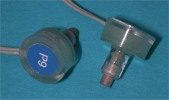
\includegraphics[width=0.325\textwidth]{bilder/Pin-Elektroden.jpg}
    \quelle{\cite{biosemi_active_electrodes}.}
   \caption{Die Elektroden, die im BioSemi-System genutzt werden}
   \label{pinelectroden}
\end{figure}

Als Ground- und Referenzelektroden wurde ein Kreis aus einer Common-Mode-Sense-Elektrode (\acrshort{cms}) und einer Driven-Right-Leg-Elektrode (\acrshort{drl}) genutzt. Dabei wurde die \acrshort{cms}-Elektrode in der Mitte aller messenden Elektroden angebracht und die \acrshort{drl}-Elektrode entfernt vom Kopf, zum Beispiel am Bein oder Arm.\footnote{Vgl. \cite{biosemi_systems}} \newline
Ein Teil der Messungen (vgl. Abschnitt~\ref{sec:bedingungen}) fand in einer speziellen, für \acrshortpl{eeg} ausgelegten Kabine (4400 A-CT-Special) von Industrial Acoustics statt.\footnote{Vgl. \cite{iac_eeg_kabine}} Sie ist schwach beleuchtet, elektrisch isoliert und schallgedämpft, um die Aufnahme äußerer, nichtmenschlicher elektrischer Signale zu minimieren. In den Versuchsbedingungen s2 und s3 legte die Versuchsperson ihren Kopf in eine Kinnstütze und hatte dadurch einen konstanten Abstand von 90\,cm zum Monitor, auf dem die Experimente präsentiert wurden (vgl. Abschnitt~\ref{sec:bedingungen}).\newline

Das portable \acrshort{eeg}-Gerät, das validiert werden sollte, ist das Ultracortex Mark IV von OpenBCI. Es besteht aus einer 3D-gedruckten Halterung, welche auf das 10-20-System ausgelegt ist, in die 16 Silber-Silberchlorid-Elektroden eingesetzt werden. 14 davon sind trocken und mit spitzen Zacken versehen, um durch das Haar zu dringen. Die restlichen zwei sind ebenfalls trocken, haben aber keine Zacken, um auf die Haut aufgelegt zu werden und nicht zu verletzen. Sie werden an der Stirn angebracht. Alle Elektroden haben eine Lebensdauer von etwa zehn Nutzungen ohne Pflege, da die Beschichtung abgenutzt wird und sie schlechter leitet. Um eine korrekte Messung zu garantieren, müssen sie regelmäßig ausgetauscht werden.\footnote{Vgl. \cite{openbci_dry_electrodes}}\newline 
Zusätzlich zu den messenden Elektroden enthält das System zwei Ohrclips, die als Referenzelektroden fungieren und an einer Stelle mit möglichst wenig Hirnaktivität sitzen.\footnote{Vgl. \cite{openbci_ultracortex_shop}} Für die Auswertung wurden die Daten beider Systeme allerdings auf eine gemeinsame Durchschnittsreferenz umgerechnet (vgl. Abschnitt~\ref{sec:vorverarbeitung}). Verbunden werden die Elektroden mit Kabeln, die zu einer Platine führen, die die gesammelten Daten über Bluetooth an ein verbundenes Gerät schickt. Der Aufbau ist in Abbildung \ref{headset} zu sehen. \newline

\begin{figure}
	\centering
	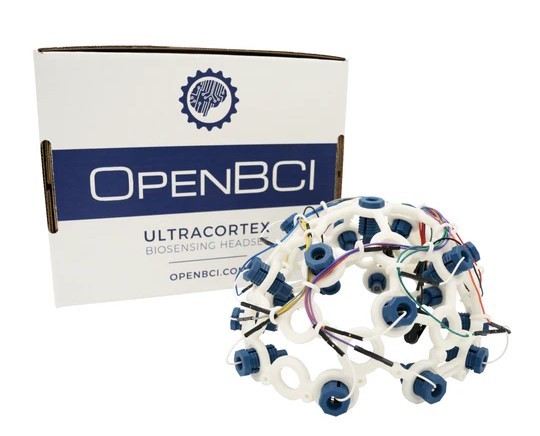
\includegraphics[width=0.325\textwidth]{bilder/Ultracortex_Headset.jpg}
   \quelle{\cite{openbci_ultracortex_shop}.}
    \caption{Das Ultracortex Mark IV Headset}
    \label{headset}
\end{figure}

\section{Beschreibung der Stichprobe} 
\autor{Lorenz Kobylka}

Geplant war die Teilnahme von 10--15 Versuchspersonen; an der Studie im Juli 2026 nahmen zehn Versuchspersonen teil. Sie waren zwischen 16 und 18 Jahren alt und besuchten das Carl-Zeiss-Gymnasium in der elften Klasse. Bevor ein \acrshort{eeg} aufgenommen wurde, unterschrieben die Versuchspersonen eine schriftliche Einverständniserklärung, füllten einen Händigkeitsfragebogen aus und gaben demografische Daten, wie Alter und Geschlecht, an. Ein genehmigter Ethik-Antrag unterstützte das Aufnehmen von Daten von Minderjährigen. Die Versuchspersonen absolvierten \acrshort{eeg}-Messungen unter drei verschiedenen Bedingungen, die jeweils etwa zehn Minuten dauerten.

\section{Experimentalaufbau für die Messung} 
\autor{Lorenz Kobylka}
\subsection{Versuchsbedingungen}
\label{sec:bedingungen}
Unsere Datenerhebung gliederte sich in drei Versuchsbedingungen, die von den Versuchspersonen durchlaufen wurden. Die Versuchsbedingungen waren dabei folgendermaßen aufgebaut: \\
\begin{tabularx}{\textwidth}{@{}lX@{}}
-- \textbf{Versuchsbedingung 1 (s1):} & Die Messung fand mit dem OpenBCI-System und ohne Kinnstütze statt, zudem stand die Tür der speziellen Kabine offen, um möglichst alltagsnahe Situationen zu simulieren.  \\
-- \textbf{Versuchsbedingung 2 (s2):} & Die Messung fand mit dem OpenBCI-System statt, nun mit einer Kinnstütze, und die Tür der Kabine war geschlossen. \\
-- \textbf{Versuchsbedingung 3 (s3):} & Die Messung fand mit dem BioSemi-System statt, unter idealen Bedingungen, d.\,h. die Kabine war geschlossen und die Versuchsperson befand sich in einer Kinnstütze. \\
\end{tabularx}
Dabei wurde zudem darauf geachtet, dass die Rahmenbedingungen konstant waren. Das beinhaltete gleichbleibende Beleuchtungsstärke und einen konstanten Geräuschpegel.


\subsection{Messung mit dem BioSemi-System}
\label{sec:messung_biosemi}
Zur Erhebung der \acrshort{eeg}-Daten wurden den Versuchspersonen verschiedene Spielkarten aus einem Pokerdeck auf einem Bildschirm gezeigt. Die Karten dienten als \gls{stimulus}. Jede Karte erschien zweimal, einmal in großer Darstellung und einmal deutlich verkleinert mit reduziertem Kontrast. Mit dem Erscheinen jeder Karte wurde ein zeitlicher Marker in den \acrshort{eeg}-Rohdaten gesetzt. Dies war ein wichtiger Bestandteil der Messung und half uns dabei, während der Auswertung genau zu bestimmen, wann das Bild gezeigt wurde und wie die entsprechende Reaktion darauf ausfiel. Denn nach der Präsentation eines Bildes tritt innerhalb der nächsten Millisekunden ein visuelles \acrshort{erp} (\Romannum{1}) auf. Dies ist gekennzeichnet durch einen charakteristischen Verlauf. Dabei ist eine bestimmte Komponente in diesem Verlauf für unsere Auswertungsmethode entscheidend: die sogenannte P1. Diese spiegelt die Verarbeitung des visuellen Reizes wider und reagiert sensibel auf Unterschiede in Größe und Kontrast der dargebotenen Reize. Entsprechend wurde erwartet, dass sich die P1-Antwort zwischen den beiden Darbietungsbedingungen deutlich unterscheidet.\newline
Ein einzelner Durchgang begann mit der Präsentation eines Fixationskreuzes für 500\,ms, gefolgt von der Anzeige einer Spielkarte für 750\,ms. Anschließend erschien für 2000\,ms ein schwarzer Bildschirm. Um die Aufmerksamkeit der Versuchspersonen sicherzustellen, sollten sie bei jedem gezeigten König die Leertaste drücken. Insgesamt wurden 104 Karten präsentiert (52 Karten eines Pokerdecks in zweifacher Wiederholung), was eine Dauer von etwa fünf Minuten ergab.\newline
Um die Alpha-Power messen zu können (\Romannum{2}), wurde das \acrshort{eeg} einmal mit geschlossenen Augen aufgezeichnet und anschließend mit geöffneten. Zwischen diesen Bedingungen sollte ein großer Unterschied in der Alpha-Power zu sehen sein (vgl. Abschnitt~\ref{sec:alpha}). Diese Messung, inklusive Instruktion, dauerte drei Minuten.




    \subsection{Messung mit dem OpenBCI-System}

Zur Erhebung der \acrshort{eeg}-Daten durchliefen die Versuchspersonen den bereits in Abschnitt~\ref{sec:messung_biosemi} beschriebenen Untersuchungsablauf, wobei die gleichen Aufgaben bearbeitet wurden und sich lediglich die eingesetzten Messinstrumente unterschieden. Zuerst durchlief die Versuchsperson die Versuchsbedingung s1. Diese Daten wurden aufgezeichnet und gespeichert. Im Anschluss folgte s2.

  

    \subsection{Zeitlicher Ablauf des Experiments} 
\autor{Lorenz Kobylka}

Der Ablauf sah dabei folgendermaßen aus: 

    \begin{itemize}
\item Ankommen der Versuchspersonen \& Unterschreiben einer Einverständniserklärung (ca. 5 min)
\item Erhebung der demografischen Daten (ca. 10 min)
\item Anlegen und Prüfen des OpenBCI-Systems (ca. 10 min)
\begin{itemize}
\item \textbf{s1} (ca. 10 min)
\item \textbf{s2} (ca. 10 min)
\end{itemize}
\item Abnehmen des OpenBCI-Systems und Anlegen des BioSemi-Systems mit 32 Elektroden (ca. 25 min)
\begin{itemize}
\item \textbf{s3} (ca. 10 min)
\end{itemize}
\item Abnehmen des BioSemi-Systems (ca. 5 min)
\item Haare waschen (ca. 10 min)
\item Belohnung, Auswertung, aufkommende Fragen besprechen, Verabschiedung der Versuchspersonen (ca. 10 min) 

\end{itemize}

Für die Datenerhebung mit unseren Versuchspersonen war eine Gesamtdauer von etwa 110 Minuten pro Person eingeplant. Diese Zeit umfasste sowohl die eigentliche \acrshort{eeg}-Messung als auch die Vor- und Nachbereitung im Labor.
\section{Auswertungsmethodik}
\label{sec:auswertung}
\autor{Alisa Fiedler}

Die im vorangegangenen Abschnitt beschriebenen Rohdaten wurden für beide Zielgrößen -- die P1-Komponente und die Alpha-Power -- zunächst gemeinsam vorverarbeitet und anschließend in zwei getrennten Auswertungssträngen analysiert. Der grundsätzliche Ablauf ist in Abbildung~\ref{analysis} dargestellt.


\begin{figure}[h]
	\centering
	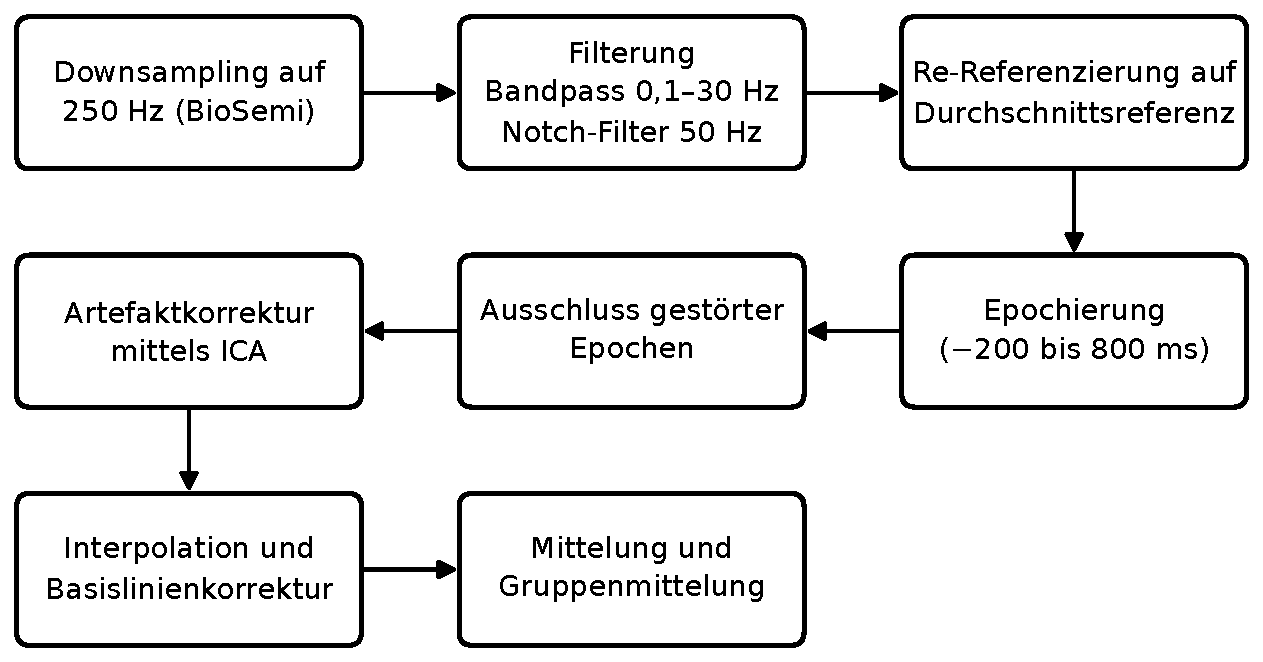
\includegraphics[width=0.85\textwidth]{bilder/Analysis_Pipeline}
    \quelle{Eigene Abbildung.}
    \caption{Auswertungsstränge}
    \label{analysis}
\end{figure}


\subsection{Vorverarbeitung der Rohdaten}
\label{sec:vorverarbeitung}
Vor der eigentlichen Analyse wurden die Rohdaten für jede Versuchsperson mit einem \gls{bandpass} gefiltert und mit einem \gls{notch} vom 50-Hz-Netzbrummen befreit (vgl. Abschnitt~\ref{sec:stoer}). Da sich die Anforderungen der beiden Zielgrößen unterscheiden, erhielt jeder Auswertungsstrang eigene Filtergrenzen: 0,1--30\,Hz für die \acrshortpl{erp}, die eine feine zeitliche Auflösung im niederfrequenten Bereich benötigen, und 1--40\,Hz für die Alpha-Power. Danach erfolgte eine Re-Referenzierung auf die \gls{durchschnittsreferenz}. Dies war für diese Arbeit notwendig, da das OpenBCI-System gegen die Ohrclips als Referenz misst, während das BioSemi-System die \acrshort{cms}- und \acrshort{drl}-Elektroden als Referenz nutzt (vgl. Abschnitt~\ref{sec:stoer}). Durch die gemeinsame Durchschnittsreferenz sind die Daten beider Systeme auf dieselbe Weise referenziert.\newline

Elektroden, die vor oder während der Messung als defekt oder stark verrauscht auffielen, wurden markiert und aus den benachbarten Elektroden mittels \gls{spline} rechnerisch ersetzt (Interpolation).\footnote{Vgl. \cite{ferree_spherical}} So hatten alle Versuchspersonen dieselbe Anzahl an Kanälen, was eine Gruppenmittelung ermöglicht. Beim OpenBCI-System betraf dies in den auswertbaren Datensätzen im Mittel etwa 7 der 16 Elektroden, vor allem frontale Elektroden wie F3, F4 und F7 sowie P4. 

\subsection {Vorverarbeitung der Rohdaten: Ergänzungen für OpenBCI}
\label{sec:openbci_trigger}
\autor{Sophie Kleppe}

Das \gls{openbci-board} wurde über die Software \gls{brainflow} ausgelesen.
BrainFlow speichert die Daten als Textdatei im \gls{Comma-Separated Values} (\acrshort{csv}) mit 32
Spalten. Enthalten sind die Kanäle 1--16, wobei die Spannungen in \textmu V angegeben
sind. Weitere Spalten enthalten den Zeitstempel des Computers und eine Spalte
für die \glspl{trigger}. Jede Zeile der Datei entspricht einem Messzeitpunkt.
Das OpenBCI-System zeichnet pro Elektrode 125 Messwerte pro Sekunde auf, was
einer \gls{abtastrate} von 125\,Hz entspricht (BioSemi: 512\,Hz). Damit die
OpenBCI-Daten auf dieselbe Weise wie die BioSemi-Daten mit \gls{mne}
ausgewertet werden können, wurden sie in das BioSemi Data Format
umgewandelt, in dem auch die Daten des BioSemi-Systems gespeichert sind. Bei
dieser Umwandlung gingen die Trigger verloren, und die Signale wurden
abgeschnitten. Zusätzlich kam es zu einem Problem bei der zeitlichen
Zuordnung der Trigger. BrainFlow empfängt die Messwerte nicht
einzeln, sondern in Paketen von jeweils 60 Messwerten. Da das System 125
Messwerte pro Sekunde aufzeichnet, umfasst ein Paket einen Zeitraum von
0,48\,s. Ein Trigger kann so allerdings nicht dem Messzeitpunkt, an dem
der Stimulus erscheint, zugeordnet werden, sondern erst dem ersten
Messwert des nächsten Pakets. Die Trigger liegen daher zufällig
zwischen 0 und 480\,ms nach dem tatsächlichen Stimulusbeginn.

Dies führt zu einem Problem bei der Auswertung der P1. Da die P1 ein kurzer
Ausschlag von etwa 50\,ms ist, der nur sichtbar wird, wenn viele \glspl{epoche} genau
zum Stimulusbeginn übereinandergelegt und gemittelt werden, würden die zufällig
verschobenen Trigger dazu führen, dass die P1 bei der Mittelung
zeitlich verschmiert. Um dieses Problem zu lösen, waren umfangreiche
Programmierarbeiten in Python nötig, die über unsere eigenen
Programmierkenntnisse hinausgingen. Deshalb wurde der KI-Assistent
\gls{claude-code} (Anthropic) eingesetzt, um ein Python-Skript zur
Rekonstruktion des tatsächlichen Stimulusbeginns zu entwickeln. Dies erfolgte
durch die Kombination zweier Informationen. Zum einen hält das
Präsentationsprogramm PsychoPy für jeden Durchgang genau fest, zu welchem
Zeitpunkt der Stimulus erscheint, woraus sich die Abstände zwischen allen
Stimuli einer Messung ergeben. Aus der \acrshort{eeg}-Aufzeichnung lässt sich dagegen nur
ablesen, in welchem Zeitraum ein Stimulus erscheint. Weil der
Trigger erst mit dem nächsten Paket gespeichert wird, liegt der
tatsächliche Stimulusbeginn innerhalb der 0,48\,s davor. Zu klären war also,
um wie viel die beiden Zeitachsen gegeneinander verschoben waren. Dafür wurde
eine Verschiebung gesucht, bei der alle Stimuli einer Messung gleichzeitig in
das 0,48-s-Fenster fallen. Bei rund 100 Stimuli mit bekannten Abständen konnte
der zeitliche Versatz deshalb sehr genau eingegrenzt werden. Im Median
verblieb jedoch eine mögliche Abweichung von 8,6\,ms. Diese ist im Vergleich
zur Dauer der P1 klein und genügte deshalb für die Auswertung. Als Kontrolle
wurden mit derselben Zuordnung die Zeitpunkte der Tastendrücke vorhergesagt,
die meist auf 0 bis 9\,ms mit den aufgezeichneten Triggern
übereinstimmten.

Nach der Rekonstruktion der Trigger erfolgte die bereits beschriebene Analyse. Alle Entscheidungen zur Auswertung wurden von uns
getroffen, und die Ergebnisse der von \gls{claude-code} erstellten Programme
wurden von uns überprüft. Zusätzlich wurden die Ergebnisse von
Wissenschaftlerinnen und Wissenschaftlern des Instituts für Psychologie
kontrolliert.


\subsection{Auswertung der P1}
\label{sec:p1auswertung}
\autor{Alisa Fiedler}

Da einzelne Aktionspotenziale und selbst einzelne ereigniskorrelierte Antworten im fortlaufenden \acrshort{eeg} nicht direkt erkennbar sind, sondern von deutlich größeren Hintergrundschwankungen überlagert werden (vgl. Abschnitt~\ref{sec:erp}), lässt sich die P1-Komponente nicht aus einer einzelnen Reizsetzung ablesen. Sie muss stattdessen aus vielen gleichartigen Reizwiederholungen herausgemittelt werden. Die Auswertung der P1-Komponente gliederte sich deshalb in mehrere aufeinanderfolgende Schritte, die zunächst pro Versuchsperson und erst am Ende über die gesamte Stichprobe hinweg durchgeführt wurden.

\textbf{Epochierung:} Zunächst wurde die fortlaufende Aufzeichnung jeder Versuchsperson um jeden einzelnen Bildreiz herum in kurze Ausschnitte, sogenannte \glspl{epoche}, zerschnitten. Jede Epoche reichte von 200\,ms vor bis 800\,ms nach dem Reizbeginn, sodass sowohl ein Referenzzeitraum vor dem Reiz als auch der gesamte relevante Antwortverlauf danach erfasst wurde. Die beiden Darbietungsbedingungen groß, kontrastreich und klein, kontrastreduziert (vgl. Abschnitt~\ref{sec:messung_biosemi}) wurden dabei von Anfang an getrennt gehalten, da sie später getrennt gemittelt und miteinander verglichen werden sollten.


\textbf{Ausschluss gestörter Epochen:} Nicht jede Epoche eignet sich für die weitere Auswertung: Bewegt sich eine Versuchsperson, verspannt sie die Kiefer- oder Nackenmuskulatur oder löst sich kurzzeitig eine Elektrode, entstehen große, kurzzeitige Spannungsausschläge, die das später berechnete Mittel verzerren würden. Anstatt solche Epochen anhand eines einzelnen, fest gewählten Amplitudengrenzwerts automatisch zu verwerfen, wurden alle Epochen visuell durchgesehen und einzeln beurteilt. Diese Vorgehensweise wurde gewählt, da ein fester Schwellenwert bei realen, unterschiedlich stark verrauschten Aufzeichnungen entweder zu viele unauffällige Epochen mitverwirft oder zu viele gestörte Epochen durchlässt. Die visuelle Beurteilung erlaubt es dagegen, für jede Epoche einzeln zwischen echten Artefakten und normaler Signalvariabilität zu unterscheiden. Die Epochen, die als gestört erkannt wurden, wurden aus der weiteren Analyse ausgeschlossen. Im Mittel gingen pro Versuchsperson und Darbietungsform etwa 48 der 52 Epochen in die weitere Auswertung ein. 


\textbf{Artefaktkorrektur mittels \acrshort{ica}:} Im nächsten Schritt wurde eine \acrshort{ica} (vgl. Abschnitt~\ref{sec:stoer}) auf die verbleibenden Epochen angewendet. Einige Störquellen zeigen dabei typische räumliche und zeitliche Muster. So erzeugen Lidschläge starke Ausschläge, die vor allem an der Stirn konzentriert sind. Horizontale Augenbewegungen zeigen sich als entgegengesetzte Signale auf beiden Stirnseiten, und Muskelanspannung äußert sich als hochfrequentes Rauschen an den Elektroden in Ohrnähe. Aufgrund dieser Muster kann man einzelne Komponenten eindeutig bestimmten Artefakttypen zuordnen. Nur die Komponenten, die als Artefakt identifiziert wurden, wurden aus dem Signal entfernt. Alle anderen Komponenten sowie die eigentliche Hirnaktivität blieben unverändert erhalten. Dieser Schritt ist wichtig, weil Lidschlagartefakte oft um ein Vielfaches größer sind als die eigentliche P1-Amplitude. Ohne Korrektur würden solche Artefakte jede Mittelung verzerren.


\textbf{Interpolation und Basislinienkorrektur:} Markierte Elektroden wurden nun interpoliert (vgl. Abschnitt~\ref{sec:vorverarbeitung}). Danach wurde die Basislinie korrigiert, wobei von jeder Epoche der Mittelwert des Zeitraums von $-$200 bis 0\,ms abgezogen wurde. Diese Reihenfolge wurde absichtlich gewählt. Würde die Basislinie vor der Bereinigung der Artefakte berechnet, könnte sie selbst durch Störungen beeinflusst sein, die später im \acrshort{ica}-Schritt entfernt werden. Dann würde die gesamte Epoche nach dieser falschen Nulllinie bewertet.


\textbf{Mittelung und Gruppenmittelung:} Für jede Versuchsperson wurden die verbleibenden, bereinigten Epochen nach der Bedingung getrennt gemittelt. So entstand für jede Person und jede Bedingung ein eigener \acrshort{erp}-Verlauf. Diese einzelnen Verläufe wurden dann über alle Versuchspersonen hinweg zusammengefasst, um eine Gruppenmittelung zu erhalten. Diese Gruppenmittelung wird auch \gls{grand-average} genannt. Die Mittelung auf zwei Stufen -- erst innerhalb jeder Person, dann zwischen den Versuchspersonen -- sorgt dafür, dass jede Person gleich stark in das Gesamtergebnis einfließt, unabhängig davon, wie viele gültige Epochen sie hat.


\textbf{Auswertungsregion und Zeitfenster:} Es wurde gezielt die okzipito-parietale Elektrodenregion (O1, O2, P7, P8) ausgewertet, weil dort die P1-Komponente normalerweise am stärksten zu sehen ist. Diese Analyse erfolgte innerhalb eines Zeitfensters von 80--200\,ms, das den Gipfel der P1-Komponente bei beiden Systemen vollständig umfasst (vgl. Abschnitt~\ref{sec:erp}). Die Auswertung beschränkte sich auf diese Region und dieses Zeitfenster, statt alle Elektroden über den gesamten Zeitverlauf zu betrachten. Das verhindert, dass zufällige Schwankungen an Stellen oder zu Zeiten, die nicht relevant sind, fälschlicherweise als Wirkung gedeutet werden.


\textbf{Kennwert der P1:} Um die P1 zwischen verschiedenen Bedingungen und Systemen zu vergleichen, kommen im Analysefenster zwei Kennwerte infrage: ihre Amplitude, also wie stark der Ausschlag ist, und ihre Latenz, also wann dieser Ausschlag stattfindet. Zwei verschiedene Vorgehensweisen sind hier möglich. Bei der Spitzenwert-Methode wird direkt im Analysefenster der höchste gemessene Wert und der Zeitpunkt dafür ermittelt. Diese Methode ist einfach zu verstehen, kann aber empfindlich auf Rauschspitzen reagieren, die den Peak leicht verfälschen können. Bei der Mittelwert-Methode hingegen wird der Durchschnitt aller Werte im Analysefenster berechnet. Diese Methode ist robuster gegenüber Ausreißern, liefert aber keine direkte Angabe zur Latenz. In dieser Arbeit wurde die Amplitude mit der Mittelwert-Methode im Zeitfenster von 80--200\,ms bestimmt, da sie robuster gegenüber Rauschen ist. Die Latenz wurde nicht ausgewertet, da das OpenBCI-System bei 125\,Hz nur alle 8\,ms einen Messwert liefert und seine Kurven durch die Rekonstruktion der Trigger zeitlich gegenüber dem BioSemi-System versetzt sein können (vgl. Abschnitt~\ref{sec:openbci_trigger}). Für alle Bedingungen und beide Systeme wurde dieselbe Methode genutzt, damit Unterschiede in den Werten tatsächlich auf das Signal selbst zurückzuführen sind und nicht auf die Art der Auswertung.

\textbf{Grundrauschen und \acrshort{snr}:} Zur Abschätzung des Grundrauschens wurde für jede Versuchsperson die Standardabweichung des gemittelten \acrshort{erp} im Basislinienintervall ($-$200 bis 0\,ms) bestimmt. Als \acrshort{snr} wurde das Verhältnis aus mittlerer P1-Amplitude und dieser Standardabweichung berechnet.


\textbf{Latenzvariabilität zwischen Versuchspersonen:} Bei der Bildung der Gruppenmittelung entsteht ein methodisches Problem: Die P1 tritt bei jeder Versuchsperson nicht exakt zum selben Zeitpunkt auf, sondern ist um wenige Millisekunden nach vorn oder hinten verschoben. Diese individuellen Zeitverschiebungen werden als Latenz-Jitter bezeichnet. Mittelt man die einzelnen Kurvenverläufe direkt, ohne diesen Jitter zu berücksichtigen, überlagern sich die leicht versetzten Spitzen der Versuchspersonen nicht mehr exakt, sondern \glqq verschmieren\grqq{} sich gegenseitig; die in der Gruppenmittelung sichtbare Amplitude fällt dadurch systematisch kleiner aus, als sie bei den einzelnen Personen tatsächlich ist. Um diesen Effekt zu vermeiden, wurde die Amplitude deshalb nicht direkt an der Gruppenmittelung abgelesen, sondern zunächst getrennt für jede einzelne Versuchsperson bestimmt; erst diese individuellen Werte wurden anschließend über die Stichprobe gemittelt beziehungsweise statistisch verglichen. Die Gruppenmittelung selbst diente in diesem Vorgehen vor allem der visuellen Kontrolle und grafischen Darstellung des typischen Kurvenverlaufs, nicht jedoch der eigentlichen Kennwertbestimmung.

\textbf{Kontrastvergleich:} Abschließend wurden die mittleren P1-Amplituden der Darbietungsbedingungen groß, kontrastreich und klein, kontrastreduziert für jede Versuchsbedingung miteinander verglichen. Dieser Vergleich dient als Kriterium dafür, ob ein System die P1 klar erkennbar abbildet (vgl. Abschnitt~\ref{sec:fragestellung}).





\subsection{Auswertung der Alpha-Power}
\label{sec:alphaauswertung}
\autor{Lorenz Kobylka}
Die Auswertung gliederte sich in zwei Ebenen und einzelne Teilschritte. Nach der Vorverarbeitung mit einem Bandpass von 1--40\,Hz (vgl. Abschnitt~\ref{sec:vorverarbeitung}) wurden zunächst die Bereiche extrahiert, bei denen die Versuchsperson die Augen geöffnet (\acrshort{eo}) hatte und wo sie die Augen geschlossen (\acrshort{ec}) hatte. Hierbei wurden im Gegensatz zu der \acrshort{erp}-Analyse keine kurzen Epochen ausgeschnitten, sondern längere zusammenhängende Blöcke. \newline

Zur genaueren Untersuchung wurde nun die \gls{psdgl} (\acrshort{psd}) mittels der \gls{welch}\footnote{Vgl. \cite{welch1967}} für jede Versuchsperson für Augen geöffnet und Augen geschlossen berechnet. Dabei ist wichtig zu erwähnen, dass die \acrshort{psd} über das gesamte Spektrum berechnet wurde und nicht nur über das Alpha-Band.  Dadurch ist es möglich, die Stärke der Alpha-Aktivität in diesen Blöcken zu quantifizieren und somit zu vergleichen. Diese \acrshortpl{psd} wurden dann über alle Versuchspersonen, frequenzweise und kanalweise, gemittelt. Aus diesen gemittelten Spektren wurde der Mittelwert im Alpha-Band (8--12\,Hz) gezogen, einmal für die Bedingung Augen offen und einmal für die Bedingung Augen geschlossen. Dieser Mittelwert wird als Alpha-Power bezeichnet und gibt in der Einheit \textmu V$^2$/Hz an, wie stark die Alpha-Aktivität ist. Anschließend wurde das Verhältnis \acrshort{ec}/\acrshort{eo} gebildet, das als Alpha-Suppression bezeichnet wird. Ist der Wert größer als 1, ist die Alpha-Aktivität bei geschlossenen Augen stärker als bei offenen. Die Kanäle wurden mittles \glspl{elektrodencluster} zu Kopfregionen zusammengefasst, deren mittlere Verhältnisse verglichen wurden, wobei ein besonderer Fokus auf der okzipitalen Region lag (okzipital: O1, O2; parietal: P3, P7, P8; zentral: C3, C4; frontal: Fp1, F8). Die Alpha-Power der einzelnen Versuchspersonen sowie deren Rangfolge wurden dagegen über die okzipito-parietale Region (O1, O2, P7, P8) gemittelt, also über dieselben Elektroden wie bei der P1-Auswertung.





\chapter{Ergebnisse aus der Messung}
\section{Datengrundlage}
\label{sec:datengrundlage}
\autor{Lorenz Kobylka}
Die Datengrundlage für die Auswertung des BioSemi-Systems bilden die Daten aller zehn Versuchspersonen. Für das OpenBCI-System liegen nur neun auswertbare Datensätze aus
s1 (Kabinentür offen und keine Kinnstütze) und sechs aus s2
(Kabinentür geschlossen und Kinnstütze) vor. Grund dafür ist das Ausschließen einiger
Datensätze aufgrund von Elektroden, deren Signale keine ausreichende Qualität
aufwiesen. Eine Ursache sind die Trockenelektroden des OpenBCI-Systems, welche
bei einigen Messungen keinen dauerhaft ausreichenden Kontakt zur Kopfhaut
hatten. Die Signale der betroffenen Elektroden waren dadurch entweder stark
verrauscht oder übersteuert, das heißt, sie zeigten dauerhaft den maximal
messbaren Wert an und enthielten keine verwertbare Hirnaktivität mehr. Solch
übersteuerte Elektroden werden auch als \textit{railed} bezeichnet. Einzelne
gestörte Elektroden lassen sich zwar aus den benachbarten Elektroden
rechnerisch durch Interpolation ersetzen (vgl. Abschnitt~\ref{sec:vorverarbeitung}), sind jedoch
zu viele Elektroden betroffen, ist dieses Verfahren nicht anwendbar, da die
Interpolation fehlender Kanäle aus benachbarten Elektroden voraussetzt, dass
genügend gute Nachbarkanäle vorhanden sind. Folgende Datensätze mussten
dadurch ausgeschlossen werden: in s1 der Datensatz von
pt\_06 (Versuchsperson 6) und in s2 die Datensätze von pt\_01, pt\_04,
pt\_07 und pt\_06.

Die Hirnaktivität unterscheidet sich zwischen einzelnen Personen deutlich,
beispielsweise in der Stärke der Alpha-Aktivität oder in der Amplitude der P1. Würden die Gruppenmittelungen der einzelnen Messungen mit unterschiedlichen
Versuchspersonen gebildet werden, könnte ein Unterschied zwischen den Messungen allein
darauf zurückzuführen sein, dass jeweils andere Personen in die Mittelung eingehen, und
nicht auf das verwendete \acrshort{eeg}-System oder die Versuchsbedingung. Deshalb wurden für den Vergleich der Messungen nur Versuchspersonen herangezogen, die
in allen drei Messungen gültige Daten aufweisen. 

\section{Verhaltensergebnisse}
Zur Erfassung der Verhaltensdaten wurden pro Versuchsperson im Kartendeck acht
Könige gezeigt, auf welche mit dem Drücken der Leertaste reagiert werden
sollte. Dies sollte die Aufmerksamkeit der Versuchspersonen sicherstellen. Als
Reaktionszeit wurde die Zeit zwischen dem Erscheinen eines Königs und dem
Drücken der Leertaste bestimmt. Anschließend wurde der Median der
Reaktionszeiten berechnet und dieser Wert über alle Versuchspersonen gemittelt.

Die Aufgabe wurde in allen Messungen nahezu fehlerfrei gelöst, das heißt auf alle
Könige wurde mit Drücken der Leertaste reagiert. Von 80 Königen pro Messung
wurden in s1 und s3 alle, in s2 79 Könige erkannt.
Die Reaktionszeit (Mittelwert $\pm$ \gls{standardabweichung} der individuellen
Mediane) betrug in s1 $550 \pm 68$\,ms, in s2
$589 \pm 79$\,ms und in s3 $591 \pm 70$\,ms. Die Messungen
unterschieden sich damit in der Reaktionszeit. In s2 reagierten alle
zehn Versuchspersonen langsamer als in s1, während sich s2
und s3 bezüglich des Verhaltens nicht unterschieden. Ordnet man die
Messungen nach ihrer Position in der zeitlichen Abfolge, war bei allen zehn
Versuchspersonen die jeweils erste Messung die schnellste. Die Reaktionszeit
verlängerte sich also nach der ersten Messung um etwa 40\,ms und blieb danach
konstant.
\section{Ergebnisse der ERP-Analyse}
\autor{Alisa Fiedler}

Die P1-Komponente wird für das BioSemi-System in zwei Darbietungsformen
beschrieben (groß und kontrastreich gegenüber klein und kontrastreduziert).
Für das OpenBCI-System werden zusätzlich die zwei Versuchsbedingungen
betrachtet (geschlossene versus offene Kabinentür und mit / ohne Kinnstütze). Die Auswertung erfolgt dabei
beschreibend anhand von Mittelwerten und Standardabweichungen. Auf
\glsdisp{inferenzstatistik}{inferenzstatistische Tests} wurde aufgrund des Rahmens dieser Arbeit
verzichtet. Nicht berichtet wird, ob die P1 auf der linken oder rechten
Kopfseite größer war.

\begin{table}[htbp]
  \centering
  \caption{Mittlere P1-Amplituden der beiden Darbietungsformen für das
  BioSemi- und das OpenBCI-System (Zeitfenster 80--200\,ms, Mittelwert
  $\pm$ Standardabweichung)}
  \label{tab:p1_amplituden}
  \small
  \begin{tabular}{llccc}
    \hline
    System & Bedingung & $n$ & \shortstack{groß,\\kontrastreich [\textmu V]} & \shortstack{klein,\\kontrastreduziert [\textmu V]} \\
    \hline
    OpenBCI & s1 & 6 & 1,49 $\pm$ 1,23 & 1,44 $\pm$ 1,22 \\
    OpenBCI & s2 & 6 & 2,39 $\pm$ 1,02 & 2,05 $\pm$ 1,35 \\
    BioSemi & s3 & 6 & 2,97 $\pm$ 1,90 & 2,20 $\pm$ 1,52 \\
    \hline
  \end{tabular}
  \tabquelle{Eigene Darstellung.}
\end{table}

Tabelle \ref{tab:p1_amplituden} zeigt die mittleren P1-Amplituden beider Darbietungsformen für die drei Bedingungen. In allen drei Bedingungen war die P1 für große, kontrastreiche Stimuli größer als für kleine, kontrastreduzierte Stimuli. Die Höhe der P1 unterschied sich allerdings zwischen den Versuchsbedingungen und nahm von s3 über s2 zu s1 ab. Der Unterschied der mittleren Amplituden im Zeitfenster von 80--200\,ms zwischen großen, kontrastreichen und kleinen, kontrastreduzierten Stimuli betrug beim BioSemi-System \textbf{0,77\,\textmu V}, beim OpenBCI-System in s2 \textbf{0,34\,\textmu V}  und in s1 nur noch \textbf{0,05\,\textmu V}. Größer als bei kleinen, kontrastreduzierten Stimuli war die P1 bei großen, kontrastreichen Stimuli beim BioSemi-System bei fünf, in s2 bei vier und in s1 bei zwei der sechs Versuchspersonen. Gemittelt über beide Darbietungsformen erreichte das OpenBCI-System in s2 etwa \textbf{0,86} und in s1 etwa \textbf{0,57} der Amplitude des BioSemi-Systems. Die Standardabweichungen waren unter allen Bedingungen groß. Sie betrugen beim BioSemi-System bis zu 1,90\,\textmu V und waren in s1 mit 1,23 und 1,22\,\textmu V fast so groß wie die zugehörigen Mittelwerte.

\begin{figure}[H]
	\centering
	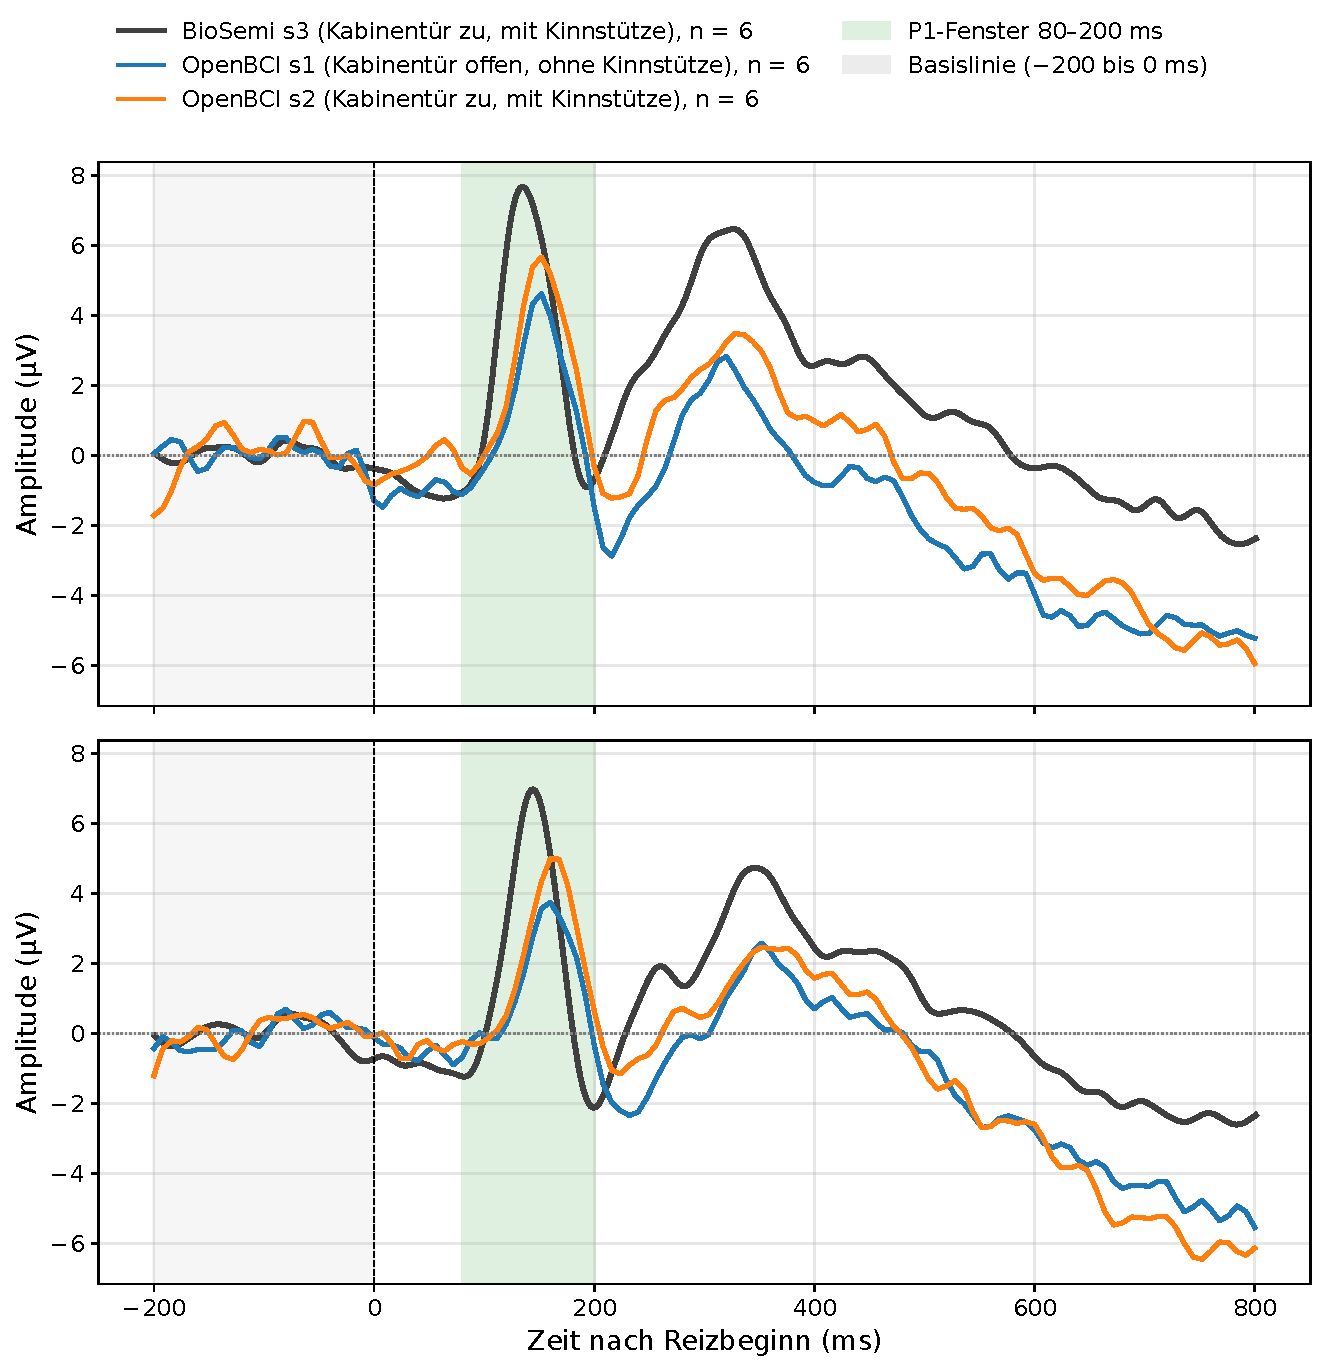
\includegraphics[width=0.95\textwidth]{diagramme/4-2_ERP_grand_average_gemeinsame6.pdf}
    \quelle{Eigene Abbildung.} 
   \caption{ERP-Grand-Average, nur Versuchspersonen mit drei gültigen Messungen, oben: groß, kontrastreich, unten: klein, kontrastreduziert}
    \label{erps_ergebnisse}
\end{figure}

Abbildung \ref{erps_ergebnisse} zeigt die über alle Versuchspersonen gemittelten Kurvenverläufe. In allen drei Bedingungen folgte auf die P1 eine Negativität um etwa 200\,ms und eine breitere Positivität zwischen etwa 300 und 350\,ms. Der grundsätzliche Verlauf stimmte damit zwischen den Systemen überein. Im Zeitraum vor dem Stimulus schwankten die OpenBCI-Kurven stärker als die BioSemi-Kurve. Ab etwa 400\,ms fielen sie zudem unter die Nulllinie ab und lagen zwischen 450 und 800\,ms im Mittel bei etwa $-$3,4\,\textmu V, während das BioSemi-Signal mit etwa $-$0,6\,\textmu V nur wenig absank.

Grundrauschen und \acrshort{snr} der P1 sind in Tabelle~\ref{tab:snr} zusammengefasst (Berechnung vgl. Abschnitt~\ref{sec:p1auswertung}). Das Grundrauschen lag beim OpenBCI-System um etwa 1,09 bis 1,46mal höher als beim BioSemi-System. Das \acrshort{snr} war beim BioSemi-System bei großen Stimuli etwa 1,9- bis 2,8-mal und bei kleinen Stimuli etwa 1,2- bis 1,9-mal so hoch wie beim OpenBCI-System. Im Mittel lag das \acrshort{snr} in allen drei Bedingungen über 1. Bei den einzelnen Versuchspersonen war dies beim BioSemi-System in 11, in s2 in 12 und in s1 in 10 von 12 Fällen (sechs Versuchspersonen mit je zwei Darbietungsformen) der Fall. Die Anzahl der gemittelten Epochen war in allen Bedingungen vergleichbar.

\begin{table}[htbp]
  \centering
  \caption{Grundrauschen (Standardabweichung der Basislinie) und \acrshort{snr} der P1 für beide Darbietungsformen (Mittelwert $\pm$ Standardabweichung)}
  \label{tab:snr}
  \small
  \begin{tabular}{llcccc}
    \hline
    System & Bedingung & \shortstack{Rauschen groß,\\kontrastreich [\textmu V]} & \shortstack{Rauschen klein,\\kontrastred. [\textmu V]} & \shortstack{\acrshort{snr} groß,\\kontrastreich} & \shortstack{\acrshort{snr} klein,\\kontrastred.} \\
    \hline
    OpenBCI & s1 & 0,79 $\pm$ 0,27 & 0,82 $\pm$ 0,39 & 1,72 $\pm$ 1,50 & 1,60 $\pm$ 0,88 \\
    OpenBCI & s2 & 0,98 $\pm$ 0,39 & 0,84 $\pm$ 0,39 & 2,53 $\pm$ 1,19 & 2,44 $\pm$ 1,21 \\
    BioSemi & s3 & 0,67 $\pm$ 0,17 & 0,75 $\pm$ 0,24 & 4,83 $\pm$ 4,05 & 3,04 $\pm$ 2,47 \\
    \hline
  \end{tabular}
  \tabquelle{Eigene Darstellung.}
\end{table}

Um grob abzuschätzen, ob die Unterschiede zwischen den Darbietungsformen über den Messfehler hinausgehen, wurde die relative Amplitudenreduktion mit dem relativen Messfehler verglichen (vgl. Abschnitt~\ref{sec:p1auswertung}). Die relative Amplitudenreduktion wurde wie folgt berechnet:

\begin{equation} \text{relative Amplitudenreduktion} = \frac{\text{P1-Amplitude für große Reize} - \text{P1-Amplitude für kleine Reize}}{\text{P1-Amplitude für große Reize}}
\end{equation}

Aus dem \acrshort{snr} lässt sich eine grobe Abschätzung für den Messfehler bestimmen. Der exakte Messfehler ist in der Praxis nicht zu errechnen, daher wird der relative Fehler als Näherung verwendet:

\begin{equation}
    \text{relativer Messfehler} \approx \frac{1}{\text{SNR}}
\end{equation}

\begin{table}[htbp]
    \centering
    \caption{Relative Amplitudenreduktion der P1, SNR und relativer Messfehler je Versuchsbedingung in Bezug auf große, kontrastreiche Stimuli}
    \label{tab:p1_reduktion}
    \begin{tabular}{cccc}
    \toprule
    Versuchsbedingung & Relative Amplitudenreduktion & SNR & Relativer Fehler \\
    \midrule
    s1 & $3{,}3\,\%$  & 1,72 & $58{,}1\,\%$ \\
    s2 & $14{,}2\,\%$ & 2,53 & $39{,}5\,\%$  \\
    s3 & $25{,}9\,\%$ & 4,83 & $20{,}7\,\%$  \\
    \bottomrule
    \end{tabular}
    \tabquelle{Eigene Darstellung.}
\end{table}

Für s1 und s2 war die relative Amplitudenreduktion geringer als der relative Messfehler, für s3 lag sie knapp darüber (Tabelle~\ref{tab:p1_reduktion}).

\section{Ergebnisse für das Alpha-Paradigma}
\autor{Lorenz Kobylka}

\subsection{Ergebnisse der Frequenzbandanalyse}
\label{sec:frequenzbandanalyse}

\begin{figure}[htbp]
	\centering
	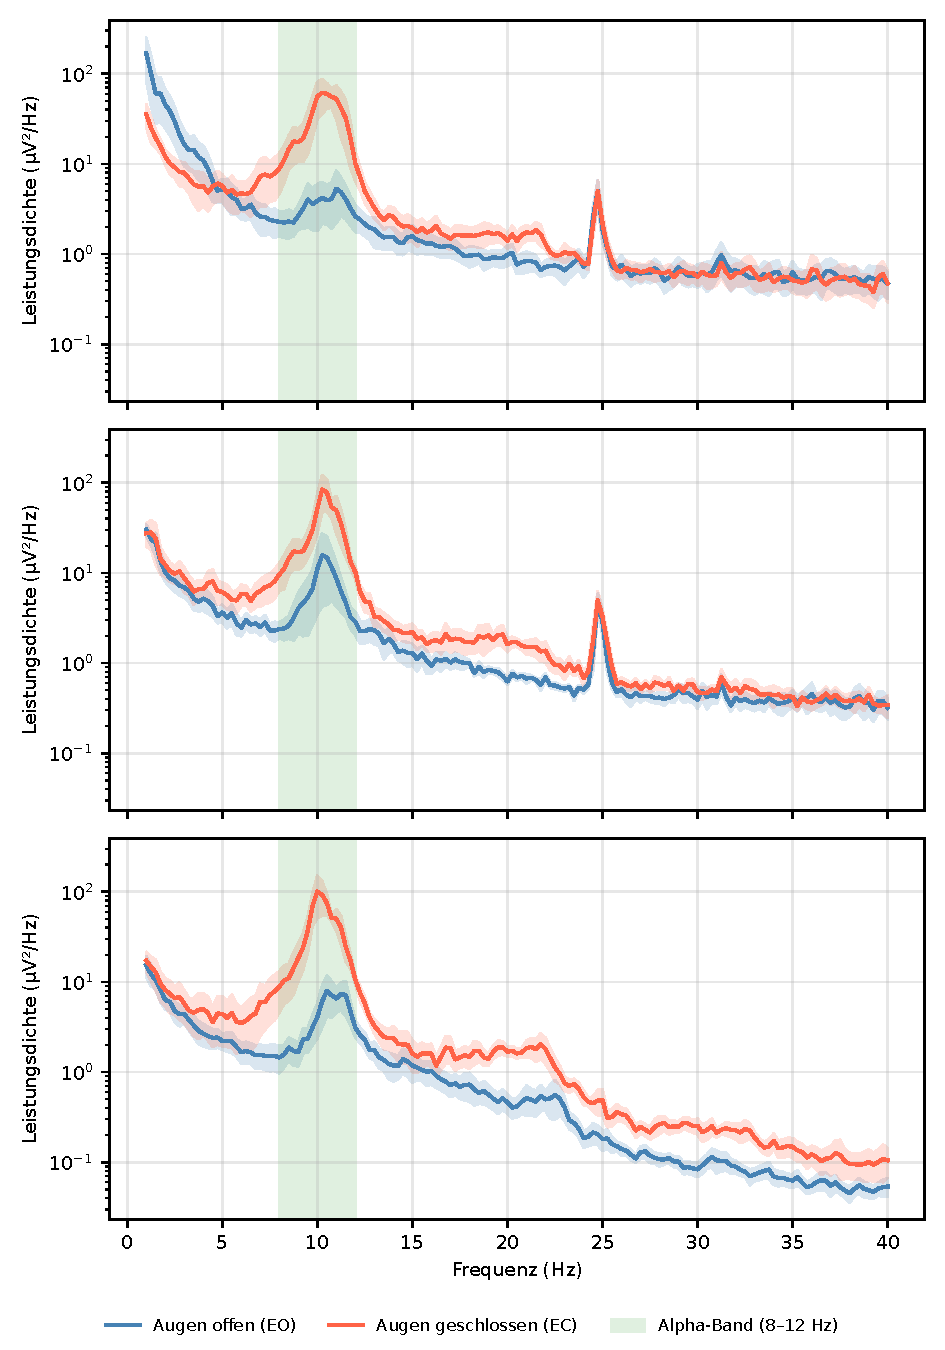
\includegraphics[width=0.85\textwidth]{diagramme/alpha_psd_okzipital.pdf}
    \quelle{Eigene Abbildung.} 
   \caption{Ergebnis der \acrshort{psd} an den okzipitalen Elektroden für alle drei Versuchsbedingungen, oben s1 (OpenBCI, Kabinentür offen), Mitte s2 (OpenBCI, Kabinentür geschlossen), unten s3 (BioSemi)}
    \label{frequenzbandanalyse}
\end{figure}

Für diesen Teil der Analyse werden ausschließlich die hinteren Elektroden über dem Okzipitallappen betrachtet (okzipitaler \gls{elektrodencluster}), da der \gls{berger-effekt} (vgl. Abschnitt~\ref{sec:alpha}) dort am stärksten ausgeprägt ist. Abbildung \ref{frequenzbandanalyse} zeigt die  \acrshort{psd} dieses Clusters als Mittelwert über alle Versuchspersonen, getrennt für die drei Versuchsbedingungen. Die \acrshort{psd} (vgl. Abschnitt~\ref{sec:alphaauswertung}) wird in \textmu V$^2$/Hz angegeben, weil die Leistung quadratisch von der Amplitude abhängt. Dadurch lässt sich die Alpha-Aktivität (8–12 Hz, grün hinterlegt) direkt ablesen.

\begin{table}[htbp]
    \centering
    \caption{Mittelwerte Alpha-Power in \textmu V$^2$/Hz bei geöffneten (EO) und geschlossenen Augen (EC) aller Versuchsbedingungen über der okzipito-parietalen Region (O1, O2, P7, P8)}
    \label{tab:alpha_power}
    \begin{tabular}{lrrrrrr}
    \toprule
     & \multicolumn{3}{c}{EO} & \multicolumn{3}{c}{EC} \\
    \cmidrule(lr){2-4} \cmidrule(lr){5-7}
    Versuchsperson & s1 & s2 & s3 & s1 & s2 & s3 \\
    \midrule
    pt\_02 & $5{,}90$ & $13{,}88$ & $6{,}22$ & $34{,}90$ & $35{,}69$ & $44{,}65$ \\
    pt\_03 & $1{,}32$ & $1{,}80$  & $1{,}36$ & $11{,}31$ & $9{,}10$  & $23{,}79$ \\
    pt\_05 & $2{,}43$ & $3{,}25$  & $3{,}19$ & $24{,}79$ & $19{,}42$ & $16{,}70$ \\
    pt\_08 & $4{,}96$ & $5{,}22$  & $6{,}73$ & $28{,}83$ & $33{,}30$ & $55{,}26$ \\
    pt\_09 & $1{,}79$ & $5{,}34$  & $3{,}06$ & $12{,}79$ & $21{,}78$ & $20{,}12$ \\
    pt\_10 & $0{,}83$ & $2{,}04$  & $1{,}00$ & $11{,}10$ & $18{,}51$ & $22{,}73$ \\
    \midrule
    Mittelwert & $2{,}87$ & $5{,}26$ & $3{,}59$ & $20{,}62$ & $22{,}97$ & $30{,}54$ \\
    \bottomrule
    \end{tabular}
  \tabquelle{Eigene Darstellung.}
\end{table}
Aus dem Graphen in Abbildung \ref{frequenzbandanalyse} lässt sich bei allen drei Messungen ein Unterschied des Hochpunkts und des Verlaufs zwischen geöffneten und geschlossenen Augen erkennen, die jedoch unterschiedlich stark ausgeprägt sind.

Die Mittelwerte der Alpha-Power der einzelnen Versuchspersonen sind in Tabelle~\ref{tab:alpha_power} aufgeführt. Diese durchschnittlichen Werte sind bessere Vergleichskriterien als die Höhe des Hochpunkts, da diese besonders anfällig für Störungen ist. Die Höhe des Peaks kann durch einzelne Artefakte stark beeinflusst werden, während die mittlere Leistung über das gesamte Frequenzband hinweg berechnet wird und dadurch robuster gegenüber Störungen ist.

Der absolute Unterschied zwischen geschlossenen und geöffneten Augen war bei s1 und s2 nahezu identisch ($20{,}62 - 2{,}87 = 17{,}75$ für s1 und $22{,}97 - 5{,}26 = 17{,}71$ für s2) und deutlich geringer als bei s3 ($30{,}54 - 3{,}59 = 26{,}95$). Außerdem zeigte sich, dass die Versuchspersonen bei s2 häufig die höchste Alpha-Power bei geöffneten Augen aufwiesen (pt\_02, pt\_03, pt\_05, pt\_09 und pt\_10).

Wichtig für die Beantwortung von Hypothese 7 (Die Trefferquote der richtigen Entscheidungen über 2-Sekunden-Abschnitte liegt über 62 \%) ist nicht nur die Betrachtung des durchschnittlichen Alpha-Wertes, sondern die Betrachtung zeitlich kurzer Abschnitte (siehe Abschnitt \ref{sec:fragestellung}).

Bei allen Durchgängen lag der Wert bei mindestens 75\,\%, meist bei mindestens 90\,\% und in seltenen Fällen sogar bei 100\,\%. Die Trefferquote war mit Daten aus dem BioSemi-System durchschnittlich höher (90--95\,\%) als mit Daten aus dem OpenBCI-System (75--100\,\%) und streute weniger. Werden die durchschnittlichen Werte zwischen s1 und s3, sowie s2 und s3 verglichen, ergibt sich ein Verhältnis von s1/s3 = \textbf{1,00} und s2/s3 = \textbf{0,96}.

Darüber hinaus lagen die absoluten Werte der einzelnen Versuchspersonen in sehr unterschiedlichen Wertebereichen. So bewegte sich die Alpha-Power bei geöffneten Augen von pt\_10 zwischen $0{,}83$ und $2{,}04$, die von pt\_02 dagegen zwischen $5{,}90$ und $13{,}88$. Ein Vergleich absoluter Werte ist daher nur eingeschränkt aussagekräftig, da jede Person eine eigene \gls{baseline_alpha} besitzt. Aus diesem Grund werden im Folgenden die Rangfolge der Versuchspersonen, wenn sie nach ihren Werten bei geöffneten Augen sortiert werden, und das Verhältnis der absoluten Werte betrachtet und zwischen den Versuchsbedingungen verglichen.

\subsection{Rangfolge der Versuchspersonen}

Die Rangfolge der Versuchspersonen ist in Tabelle \ref{tab:alpha_rank} dargestellt und wird benötigt, um die zweite Hypothese (Die Rangfolge der Versuchspersonen stimmt stark überein) zu beantworten. Sortiert man die Versuchspersonen nach ihrer Alpha-Power bei geöffneten Augen über der okzipito-parietalen Region (O1, O2, P7, P8), fällt zwischen s1 und s3 eine sehr große Ähnlichkeit auf: Die Platzierungen weichen nur bei Platz eins und zwei voneinander ab. Bei s2 unterscheidet sich die Reihenfolge vor allem im mittleren Bereich (Plätze zwei bis vier) von s1 und s3. Um die Ähnlichkeit zwischen zwei Rangfolgen zu bestimmen (um das Verhältnis der Bedingungen zu quantifizieren), wird die \gls{spearman} genutzt, die einen Wert $\rho$ liefert. Für s1/s3 beträgt $\rho$ \textbf{0,94}, für s2/s3 \textbf{0,66}.

\begin{table}[H]
    \centering
    \caption{Rang der Versuchspersonen, sortiert nach der Alpha-Power bei geöffneten Augen über der okzipito-parietalen Region (O1, O2, P7, P8) für alle Versuchsbedingungen}
    \label{tab:alpha_rank}
    \begin{tabular}{lccc}
    \toprule
    Versuchsperson & s1 & s2 & s3 \\
    \midrule
    pt\_02 & 1 & 1 & 2 \\
    pt\_03 & 5 & 6 & 5 \\
    pt\_05 & 3 & 4 & 3 \\
    pt\_08 & 2 & 3 & 1 \\
    pt\_09 & 4 & 2 & 4 \\
    pt\_10 & 6 & 5 & 6 \\
    \bottomrule
    \end{tabular}
  \tabquelle{Eigene Darstellung.}
\end{table}

\subsection{Alpha-Suppression}
\label{sec:supp}

Die Alpha-Suppression wurde wie in Abschnitt~\ref{sec:alphaauswertung} beschrieben berechnet. Ein Wert von 9 bedeutet entsprechend, dass bei geschlossenen Augen neunmal höhere Alpha-Power gemessen wird als unter Normalbedingungen (Augen geöffnet). Abbildung \ref{alpha_suppression} zeigt die über alle Versuchspersonen gemittelte Alpha-Suppression für die Cluster Okzipital, Parietal, Frontal und Zentral für s1, s2 und s3.

\begin{figure}[htbp]
	\centering
	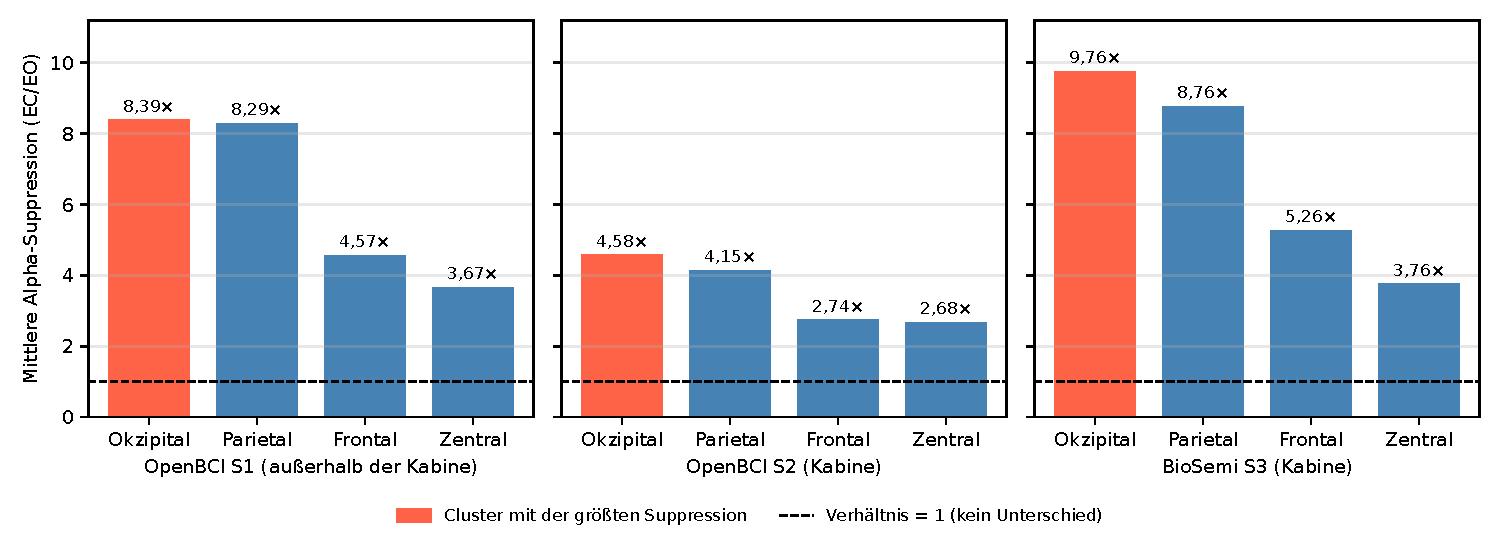
\includegraphics[width=0.85\textwidth]{diagramme/alpha_suppression_cluster.pdf}
    \quelle{Eigene Abbildung.} 
   \caption{Alpha-Suppression an den \glspl{elektrodencluster} für alle drei Versuchsbedingungen, mit Rot ist der Cluster mit größter Suppression markiert, die Linie zeigt das Kriterium Verhältnis = 2, oben s1 (OpenBCI, Kabinentür offen), Mitte s2 (OpenBCI, Kabinentür geschlossen), unten s3 (BioSemi)}
    \label{alpha_suppression}
\end{figure}

Bei allen drei Messungen war die Alpha-Suppression über dem Hinterkopf am stärksten, also über okzipitalen und parietalen Elektroden, während sie frontal und zentral deutlich geringer ausfiel. Alle Werte lagen zwischen 2 und 10. Am deutlichsten war der Unterschied zwischen den vorne und hinten liegenden Clustern beim BioSemi-System: Der okzipitale Wert (9,76) war mehr als doppelt so hoch (okzipital / zentral = 2,6) wie der zentrale (3,76) und fast doppelt so hoch wie der frontale (5,26). Bei s1 lag das Verhältnis bei 8,39 / 3,67 = 2,29. Bei s2 war die Abstufung am geringsten, der Unterschied zwischen okzipital (4,58) und frontal (2,74) war relativ gesehen kleiner (okzipital / frontal = 1,67).

Mit einer Alpha-Suppression von 9,76 lag das BioSemi-System nahe an einem Verhältnis von 10. Auch mit dem OpenBCI-System wurde in s1, mit 8,39 ein guter und nur wenig abweichender (OpenBCI / BioSemi = \textbf{0,86}) Wert erreicht.

In Abbildung~\ref{fig:alpha_suppression_pro_person} im Anhang ist eine ergänzende Grafik zur Alpha-Suppression für jede einzelne Versuchsperson dargestellt. Die Alpha-Suppression war bei jeder Versuchsperson über 2, streute aber stark zwischen 2,6 und 22,7.


\chapter{Diskussion}
\section{Bewertung der Datenqualität}
Hier werden Anomalien in den Daten sowie Umstände in der Auswertungsmethodik diskutiert. Diese können Einfluss auf die Qualität der Messergebnisse haben.\newline

Bei der Auswertung des P1-Paradigmas wird der Mittelwert der Spannung im Bereich 80--200\,ms nach dem Reiz zwischen den Systemen verglichen. Wie in Abbildung \ref{erps_ergebnisse} zu sehen, fällt die Spannung im unteren Diagramm für das BioSemi-System am Ende des betrachteten Zeitraums schneller ab als die Spannung der OpenBCI-Systeme. Das hat zur Folge, dass bei der Mittelung der Wert für das BioSemi-System geringer ist als die tatsächliche durchschnittliche Amplitude der P1. \newline
Dieser Umstand verfälscht die Daten dahingehend, dass der Wert der Spannung bei kleinen Stimuli für BioSemi größer ist als momentan berechnet. Demnach ist das Verhältnis s1/s3 und s2/s3 geringer.\newline
Bei den großen, kontrastreichen Stimuli ist der Unterschied zwischen der Negativität der Kurven kurz vor dem Ende des Intervalls sehr gering, hat also keine Auswirkung auf die Ergebnisse.\newline

Eine weitere Einschränkung der Datenqualität betrifft die zeitliche Zuordnung der Trigger beim OpenBCI-System. Da BrainFlow die Messwerte in Paketen von 60 Werten (0,48 s) empfängt, lagen die aufgezeichneten Trigger zufällig bis zu 480 ms nach dem tatsächlichen Stimulusbeginn, sodass der Stimulusbeginn nachträglich rekonstruiert werden musste (vgl. Abschnitt 3.4.2). Die Rekonstruktion ist sehr genau, ein Restfehler von im Median 8,6 ms bleibt jedoch bestehen, und die Abtastrate von 125 Hz erlaubt nur alle 8 ms einen Messwert. Verglichen mit der Dauer der P1 ist diese Abweichung klein, sodass die Auswertung möglich ist. Da die P1 jedoch nur bei exakter Überlagerung der Epochen vollständig sichtbar wird, führen bereits geringe zeitliche Verschiebungen dazu, dass die Kurven bei der Mittelung leicht zeitlich versetzt sind und die gemessene Amplitude etwas geringer ausfällt. \newline
Die niedrigeren P1-Amplituden der OpenBCI-Messungen im Vergleich zu BioSemi sind daher nicht allein auf das Messsystem selbst zurückzuführen, sondern zum Teil auch auf die Ungenauigkeit der rekonstruierten Trigger. Eine eindeutige Trennung beider Einflüsse, um die Validität der gemessenen Daten und nicht die Validität der Auswertung zu prüfen, ist anhand der vorliegenden Daten nicht möglich.\newline

Wie in den Abschnitten~\ref{sec:vorverarbeitung} und~\ref{sec:datengrundlage} beschrieben, gab es beim OpenBCI-System viele Ausfälle der Elektroden, insbesondere der frontalen. Da P1 und Alpha aber vor allem an okzipito-parietalen Elektroden ausgewertet wurden, hatte dies nur einen geringen Einfluss auf die Ergebnisse. Für eine Anwendung wie eine Station im School\_Lab ist der unzuverlässige Kontakt der Trockenelektroden jedoch eine wichtige Einschränkung. 

Bei der Frequenzbandanalyse ist eine Auffälligkeit in den Diagrammen aufgetreten.
In beiden OpenBCI-Durchläufen trat ein schmaler Peak, also ein Hochpunkt, bei 25 Hz auf, der beim BioSemi-System fehlte (in Abbildung \ref{frequenzbandanalyse} zu sehen). Er ist zu groß, zu regelmäßig und unabhängig von Augenzustand und Bedingung (keine Unterschiede in Amplitude oder Frequenz zwischen \acrshort{eo}/\acrshort{ec} sowie zwischen s1 und s2), um neuronalen Ursprungs zu sein. Auch ist nach aktuellem Stand kein physiologischer Effekt bekannt, der einen solchen Ausschlag erklären würde. Für eine technische Ursache kommen mehrere Möglichkeiten infrage:\newline
\begin{enumerate}
  \item Netzbrummen scheidet aus, da der Peak nicht bei 50 Hz liegt und sich in der Kabine keine Netzteile befinden. Gegenüber dem BioSemi-Durchlauf kam lediglich der Laptop hinzu.
  \item Bildschirmflackern: Bei Pixel-Inversion oder beim schnellen Wechsel von Pixel-Farben entsteht ein Flackern mit der halben Bildwiederholrate, bei einem 60-Hz-Monitor also bei 30 Hz. Hat der Bildschirm eine Bildwiederholrate von 50 Hz, passt diese Erklärung genau zur Beobachtung.\footnote{Vgl. \cite{flickersense_led_screens}} 
  \item Das Cyton-Board könnte aus anderen Gründen ein elektromagnetisches Feld mit 25 Hz abstrahlen.
\end{enumerate}

Mit Sicherheit lässt sich die Ursache auf Basis der vorliegenden Daten nicht bestimmen. Der Peak hat keinen Einfluss auf die Auswertung der Daten. Bei der Programmierung des Roboterarms ist jedoch zu beachten, dass diese Frequenz von 25 Hz nicht für die Bewegung des Armes genutzt werden sollte.\newline

\section{Bezug auf die Hypothesen}

\textbf{Alpha-Paradigma}\newline
Das Verhältnis zwischen den Messwerten der Alpha-Suppression zwischen OpenBCI (bei s1) und BioSemi-Gerät beträgt 0,86. Dies zeigt, dass das Alpha-Paradigma grundlegend eine gute wissenschaftliche Grundlage für eine BCI-Anwendung ist. Ob das OpenBCI-Gerät tatsächlich den \gls{berger-effekt} misst und ob die Grundlage für eine Roboterarm-Anwendung besteht, wird im Folgenden diskutiert.\newline

\textit{1) Bei beiden Systemen ist die Alpha-Power bei geschlossenen Augen bei jeder Versuchsperson größer als bei geöffneten Augen (Alpha-Suppression \acrshort{ec}/\acrshort{eo} $\geq$ 2).}\newline

Die Alpha-Suppression lag bei jeder Versuchsperson und jeder Bedingung über dem Schwellenwert von zwei (siehe Abschnitt \ref{sec:supp}, unten). Die Hypothese ist damit bestätigt.\newline
Die Suppressionen schwanken stark zwischen 2,6 und 22,7. Diese Unterschiede zwischen den Versuchspersonen sind auf die kleine Basislinie mancher Versuchspersonen zurückzuführen. Eine kleine Schwankung im Quotient zwischen den Versuchspersonen (zum Beispiel durch den Wachheitszustand) resultiert in einer großen Schwankung in der Suppression. Verstärkt wird dieser Effekt durch die quadratische Abhängigkeit der Leistung von der Amplitude der Alpha-Wellen.\newline
Würde ein durchschnittlicher Schwellenwert aus allen Versuchspersonenzur Steuerung berechnet werden, könnten Versuchspersonen mit geringer Suppression diesen nicht erreichen und der Roboterarm zu empfindlich auf geringe Alpha-Power-Schwankungen bei Versuchspersonen mit großer Suppression reagieren könnte. \newline
Deswegen muss bei der Programmierung eines Roboterarms beachtet werden, dass der Schwellenwert der Alpha-Suppression zur Initiation für eine Bewegung individuell angepasst werden sollte. \newline

\textit{2) Die Rangfolge der Versuchspersonen nach ihrer Alpha-Power stimmt zwischen den Versuchsbedingungen stark überein ($\rho \geq 0{,}5$).}\newline

Die Rangkorrelation zwischen s1 und s3 war sehr gut und liegt bei $\rho$ = 0,94, also deutlich über dem Schwellenwert von 0,5. Die Korrelation zwischen s2 und s3 lag nur bei  $\rho$ = 0,66 und ist damit zwar über dem Schwellenwert, ist aber deutlich geringer als 0,94. Die Erklärung für diesen Wert ist bei der Diskussion von Hypothese sechs gegeben.\newline 
Diese Rangfolge weist zusätzlich zu dem Verhältnis von 0,86 zwischen der Alpha-Suppression darauf hin, dass die Daten des OpenBCI-Systems ähnlich zu denen des BioSemi-Systems sind.\newline

\textit{3) Bei beiden Systemen ist die Alpha-Suppression okzipital oder parietal am größten und ist deutlich größer als die Suppression in den frontalen und zentralen Hirnregionen.}\newline

Auch diese Hypothese wird durch die Daten bestätigt (siehe Abschnitt \ref{sec:supp}). Der Unterschied zwischen am vorderen und hinteren Hirnteil iegenden Cluster war unter den drei Versuchsbedingungen unterschiedlich stark ausgeprägt (2,60 > 2,29 > 1,71). Bei s2 war der relative Unterschied der Suppression zwischen dem okzipitalen und zentralen Cluster nur 1,71. Dieser Unterschied ist zwar größer als eins (entspräche keinem Unterschied zwischen den Regionen), kann aber auch nur durch Zufall oder äußere Faktoren entstanden sein. Dies zeigt, dass die Messung unter Versuchsbedingung s2 möglicherweise nicht verwertbar ist, da hier nicht mit Sicherheit gesagt werden kann, dass diese Suppression der \gls{berger-effekt}, der physiologisch am Hinterkopf zu erwarten ist, ist und nicht ein Störsignal, welches sich auf alle Cluster auswirkt, ist. Die Begründung für diese schlechte Datenqualität bei s2 wird in der Diskussion von Hypothese sechs angebracht.\newline
Für die anderen beiden Versuchsbedingungen wurde jedoch der \gls{berger-effekt} nachgewiesen. Es ist möglich, über einen 60 Sekunden langen Abschnitt die Alpha-Suppression aufzuzeichnen und aufgrund dieser Suppression ein Steuersignal für einen Roboterarm zu senden.\newline

\textbf{P1-Paradigma}\newline
Die mittlere P1-Amplitude war bei den Messungen mit dem OpenBCI-System grundlegend geringer als beim BioSemi-System (s2/s3 = 0,86 und s1/s3 = 0,57). Das zeigt, dass das BioSemi-System ERPs und einzelne ERP-Komponenten stärker erfassen kann als das OpenBCI-System. Das liegt vermutlich an besser messenden Elektroden, keinem störenden Bluetooth-Signal und der Elektrodenanzahl. Das bedeutet weiterhin, dass das OpenBCI-System bei dem P1-Paradigma, auch unabhängig vom Rauschen, schlechtere Werte liefert als das BioSemi-System. Dieses Paradimga wird nicht als Grundlage für eine BCI-Anwendung genutzt, da der Reiz nicht von einem Menschen selbst ausgeht, sondern ein Stimulus benötigt ist. Dieses Paradigma wird lediglich zum Vergleich der Datenqualität der Systeme genutzt. Wie valide die gemessenen Daten sind, wird im Folgenden diskutiert.\newline

\textit{4) Die P1 hebt sich bei beiden Systemen vom Rauschen ab (\acrshort{snr} > 1), die \acrshort{snr} ist beim OpenBCI-System aber geringer als beim BioSemi-System.}\newline

Die SNR ist für beide Systeme in Tabelle \ref{tab:snr} dargestellt. Die SNR war durchschnittlich für beide Systeme und auch für das OpenBCI-Gerät unter alltagsnahen Bedingungen größer als eins. Es gab jedoch drei Situationen, bei denen eine Versuchsperson bei einer Versuchsbedingung eine SNR von unter eins hatte. Bei einer der Situationen wurde mit dem BioSemi-System gemessen. Deswegen ist der geringe SNR-Wert nicht besorgniserregend, da es nicht das Ziel ist, bessere Daten als das BioSemi-System zu erzeugen, also es nicht notwendig ist, dass alle Durchläufe eine SNR von über eins haben.\newline
Die SNR war für das BioSemi-System größer als für das OpenBCI-System (4,83 > 2,53 > 1,72 bei großen Stimuli und 3,04 > 2,44>1,60 bei kleinen Stimuli). Die Daten bestätigen demnach die Hypothese. Die SNR war für das OpenBCI-System deutlich geringer als für das BioSemi-System, es wurde also mehr Rauschen im Verhältnis zum Signal gemessen, wie vermutet. Dass das OpenBCI-Gerät trotzdem die P1-Komponente deutlich erfassen kann, spricht für die Validität der Daten und des Systems\newline

\textit{5) Bei beiden Systemen ist die gemessene mittlere P1-Amplitude für große, kontrastreiche Stimuli größer als für kleine, kontrastreduzierte Stimuli. Dabei ist der Unterschied beim BioSemi-System größer als beim OpenBCI-System.}\newline

Die Daten zur Einschätzung dieser Hypothese sind in Tabelle \ref{tab:p1_amplituden} und Tabelle \ref{tab:snr} zu finden. Der Unterschied zwischen großen, kontrastreichen und kleinen, kontrastreduzierten Stimuli lag bei s3, also beim BioSemi-System bei 0,77\,\textmu V und war damit mehr als doppelt so groß wie OpenBCI mit geschlossener Kabine (0,34\,\textmu V). Der Wert für s1 war im Vergleich dazu sehr gering (0,05\,\textmu V).
Wie die grobe Abschätzung des Messfehlers in Tabelle~\ref{tab:p1_reduktion} zeigt, ist für s1 und s2 die relative Amplitudenreduktion geringer als der relative Fehler. Der absolute Unterschied liegt also im Fehlerintervall. \newline
Es ist außerdem zu sehen, dass die Daten bei Bedingung 1 am wenigsten aussagekräftig sind, da der relative Fehler mehr als zehnmal so groß ist wie der gewünschte Effekt.\newline
S3 war die einzige Bedingung, bei der die Amplitudenreduktion knapp außerhalb des Fehlerintervalls liegt. Die Hypothese, es lässt sich ein Unterschied zwischen den Darbietungsformen messen, ist nur für das BioSemi-System zu bestätigen, nicht für das OpenBCI-System, selbst unter Laborbedingungen. Der absolute Unterschied ist nur der Richtung nach korrekt, aber nicht belastbar.\newline

Grund für diese Beobachtung kann ein starkes Rauschen des OpenBCI-Systems sein. Es kann in einer Folgestudie überprüft werden, ob ein größerer Kontrast zwischen den Darbietungsformen für eindeutige Messwerte mit dem OpenBCI-System sorgen würde oder ob ein derart kleiner Unterschied mit dem OpenBCI-System grundlegend nicht messbar ist. Die P1 kann zwar als Grundlage für eine Anwendung genutzt werden, allerdings ist der Unterschied zwischen verschiedenen Reizen kein guter Anhaltspunkt, um ein BCI mit dem OpenBCI-System zu erstellen.\newline

\textbf{Umgebung und Steuersignal}\newline
Hier werden zwei konkrete Aspekte zur Umsetzung eines Roboterarms-BCIs diskutiert: Die Umgebung, in der das System genutzt werden soll, und die Art des Steuersignals. \newline

\textit{6) Die Kriterien für die Datenqualität sind auch bei offener Kabinentür ohne Kinnstütze (s1) erfüllt, die Datenqualität ist bei geschlossener Kabinentür mit Kinnstütze (s2) aber besser.}\newline

Beim Auswerten des Alpha-Paradigmas fiel mehrmals auf, dass die Daten aus s2 wesentlich schlechter sind als die Daten aus s1 (siehe Hypothese 2 und 3). Das ist unerwartet, aber leicht zu erklären: Die Kabinentür war in s2 zwar geschlossen, was elektrische Störungen reduziert, aber dieser Einfluss ist gering. Einen größeren Einfluss hat die Vigilanz (allgemeine Wachheit) der Versuchspersonen. Es ist naheliegend, dass sie nach zwanzig Minuten in einem abgedunkelten Raum, wobei sie nahezu nichts tun müssen, müde werden oder sich langweilen. Beides erhöht die Alpha-Power mit geöffneten Augen, hat aber wenig Einfluss auf die Alpha-Aktivität mit geschlossenen Augen, da sich die Versuchspersonen auch nach nur zehn Minuten mit geschlossenen Augen sehr entspannen. S1 ist die zuerst durchgeführte Bedingung und liefert theoretisch die aussagekräftigste Alpha-Aktivität bei EO. \newline
S2 fand danach statt und hatte eine höhere Alpha-Aktivität bei EO (wie in Abschnitt \ref{sec:frequenzbandanalyse}, Absatz drei beschrieben), was darin resultiert, dass die Alpha-Suppression im Durchschnitt geringer ist. Die Alpha-Aktivität aufgrund Müdigkeit ist in allen Hirnregionen zu messen, deswegen ist der Unterschied zwischen den Elektroden-Clustern so gering (siehe Hypothese drei). Die Müdigkeit ist bei jeder Versuchsperson unterschiedlich stark ausgeprägt. Das spiegelt sich in der geringen Ähnlichkeit der Listen der Versuchspersonen wider (Hypothese zwei).\newline
Nach dieser Argumentation ist zu erwarten, dass die Messwerte unter Bedingung s3 noch stärker durch Müdigkeit beeinflusst sind. Dies ist jedoch nicht der Fall, die Werte sind sehr ähnlich zu s1 was Rangfolge und Alpha-Suppression betrifft. Das kann mit der Beschaffenheit und Zeitpunkt der Messung des BioSemi-Systems zu begründen sein. Es wird ein kaltes Elektrolytgel verwendet, das unangenehm kühl auf der Haut anliegt. Dieses Elektrolytgel sowie eine Umbauphase von 25 Minuten können der Grund sein, warum Müdigkeit bei s3 keinen so großen Einfluss hat wie bei s2. \newline
Anzumerken ist, dass bei Versuchsperson fünf die Reihenfolge der Bedingungen aus logistischen Gründen geändert wurde. Zuerst wurde s3 durchgeführt, dann s1 und zum Schluss s2. In diesem Fall war die Versuchsperson bei s3 am wachsten und bei s2 am müdesten, was die Datenqualität bei s2 verschlechtert und bei s3 verbessert. \newline

Hinsichtlich der s2-Messung des Alpha-Paradigmas wurde die Hypothese widerlegt. Der erste Teil der Hypothese wird jedoch bestätigt. Die Datenqualität ist bei offener Kabinentür und ohne Kinnstütze besser als bei geschlossener, allerdings liegt es dabei vermutlich nicht an den äußerlichen Bedingungen, sondern an der Vigilanz der Versuchspersonen, also einer physiologischen Änderung des Effekts. \newline
Die Müdigkeit hat jedoch keinen erkennbaren Einfluss auf das P1-Paradigma. Die Verhaltensergebnisse zeigen, dass die Versuchspersonen trotz Müdigkeit aktiv an dem Experiment teilnahmen. Bei diesem Paradigma nimmt die Datenqualität wie erwartet in der Reihenfolge s3>s2>s1 ab. Das \acrshort{snr} des OpenBCI-Systems bei geschlossener Kabine war deutlich größer als bei geöffneter Kabine mit Kinnstütze und ohne Kinnstütze (2,53>1,72 und 2,44>1,60).\newline
Die Hypothese wird für das P1-Paradigma bestätigt. Es kann vermutet werden, dass das Alpha-Paradigma die Hypothese bestätigen würde, wenn die Versuchspersonen nicht müde werden würden, aber eine begründete Aussage lässt sich nicht treffen. In Hinsicht auf die Roboterarm-Anwendung ist dies jedoch eine wichtige Erkenntnis: Das Alpha-Paradigma ist anfällig für Müdigkeit und eine Anwendung sollte anregend sein, um das Auftreten von Müdigkeit zu reduzieren.\newline

\textit{7) Mit dem OpenBCI-System lässt sich in 2-s-Abschnitten erkennen, ob die Augen geöffnet oder geschlossen waren, das heißt, die Trefferquote liegt in allen Versuchsbedingungen nicht nur über dem Zufallsniveau von 50\,\%, sondern auch über der Zufallsgrenze von 62\,\%.}\newline

Diese Hypothese lässt sich deutlich mit den gemessenen Werten, in Abschnitt \ref{sec:frequenzbandanalyse} unten, untermauern und bestätigen. Das OpenBCI-System erzielte eine Trefferquote von mindestens 75\,\%, also über dem Schwellenwert.\newline
Darüber hinaus war die Ähnlichkeit der Daten zwischen OpenBCI und BioSemi bei diesem Analyseaspekt am höchsten (1,00 beziehungsweise 0,97 bei geschlossener Kabine und müden Versuchspersonen). Daraus ergibt sich, dass ein Roboterarm mit Alpha-Aktivität über das OpenBCI-Gerät grundsätzlich gesteuert werden kann, da kurze, einfache menschliche Steuerimpulse ausreichend sind, um aus den EEG-Daten Rückschlüsse auf das Verhalten einer Versuchsperson zu ziehen. So kann ein Signal von einem Menschen an den Roboter übermittelt werden. Ob dies auch in Echtzeit zuverlässig gelingt, muss in einer Folgestudie geprüft werden.


\chapter{Fazit und Ausblick}
\autor{Sophie Kleppe}

\acrshort{bci}-Systeme können in Zukunft zu einer wegweisenden Technologie werden, die es Menschen mit Lähmungen ermöglicht, \glspl{neuroprothese} anzusteuern. Da der Einsatz im Alltag und als Experimentierstation im DLR\_School\_Lab allerdings nur mit einem portablen \acrshort{eeg}-System sinnvoll ist, war das Ziel dieser Arbeit zu prüfen, ob das OpenBCI-System auch in einer alltagsnahen Umgebung eine mit dem BioSemi-System vergleichbare Datenqualität liefert und damit als Grundlage für die Steuerung eines Roboterarms dienen kann. Um die Fragestellung zu beantworten, wurden zehn Versuchspersonen unter drei verschiedenen Versuchsbedingungen gemessen: Versuchsbedingung s1 (OpenBCI, Kabinentür offen, ohne Kinnstütze), s2 (OpenBCI, Kabinentür geschlossen, mit Kinnstütze) sowie s3 (BioSemi als Referenzsystem). Innerhalb der Versuchsbedingungen wurden zwei Paradigmen untersucht: das Alpha-Paradigma, bei dem die Augen abwechselnd geöffnet und geschlossen wurden, und das P1-Paradigma, bei dem Spielkarten groß und kontrastreich oder klein und kontrastreduziert gezeigt wurden.

Bezüglich des Alpha-Paradigmas zeigte sich, dass der \gls{berger-effekt} mit dem OpenBCI-System in allen Versuchsbedingungen deutlich messbar war, auch bei offener Kabinentür. Zudem lag die Alpha-Suppression bei allen Versuchspersonen über dem Kriterium von 2, die Alpha-Power war bei geschlossenen Augen also mindestens doppelt so hoch wie bei geöffneten. Sie war okzipito-parietal am stärksten. Die Rangfolge der Versuchspersonen stimmte stark mit der des BioSemi-Systems überein, bei offener Kabinentür stärker als bei geschlossener. Zurückzuführen ist dies vermutlich auf die zunehmende Müdigkeit der Versuchspersonen während der Messung in der geschlossenen Kabine.

Hinsichtlich des P1-Paradigmas war die P1 mit dem OpenBCI-System erkennbar und hob sich im Mittel vom Rauschen ab. Sie wies allerdings eine kleinere Amplitude auf und war stärker verrauscht. Eine mögliche Ursache ist die ungenaue Rekonstruktion der Trigger. Der Unterschied zwischen großen und kleinen Reizen war nur beim BioSemi-System belastbar. Beim OpenBCI-System lag er im Bereich des Messfehlers und kann deshalb nur als Tendenz aufgefasst werden. In der geschlossenen Kabine war die P1-Datenqualität besser als bei offener Kabinentür. Ob die Augen geöffnet oder geschlossen waren, wurde mit dem OpenBCI-System in 2-s-Abschnitten in mindestens 75\,\% der Fälle richtig erkannt, ein Ergebnis, das deutlich über der \gls{zufallsgrenze} liegt.

Für die Beantwortung der Fragestellung ergibt sich daraus, dass das OpenBCI-System für große und robuste Signale auch unter alltagsnahen Bedingungen eine ähnliche Datenqualität wie das BioSemi-System liefert. Für kleine Unterschiede in den \acrshortpl{erp} gilt dies nur eingeschränkt. Da das Öffnen und Schließen der Augen ein einfaches Steuersignal ist, das jede Person willentlich und ohne Training erzeugen kann, und bereits in Abschnitten von zwei Sekunden zuverlässig erkannt wird, kann das OpenBCI-System eine Grundlage für die Steuerung eines Roboterarms sein. Auch der Einsatz als Experimentierstation im DLR\_School\_Lab ist grundsätzlich möglich, da die Datenqualität für dieses Signal auch ohne abgeschirmte Kabine ausreicht. Allerdings gibt es auch Einschränkungen. Der Kontakt der Trockenelektroden ist nicht immer zuverlässig, sodass häufig Elektroden ausfielen und einzelne Messungen nicht auswertbar waren. Für das DLR\_School\_Lab bedeutet das, dass bei einer Station mit dem Ausfall einzelner Elektroden gerechnet werden muss. Zudem sollte die Anwendung anregend gestaltet sein, da Müdigkeit die Alpha-Aktivität beeinflusst.

Als nächster Schritt kann der Roboterarm mit dem OpenBCI-System in Echtzeit angesteuert werden. Dafür müsste die Alpha-Power während der Messung fortlaufend in kurzen Abschnitten berechnet und mit einer Schwelle verglichen werden. Wird die Schwelle überschritten, also werden die Augen geschlossen, könnte eine festgelegte Bewegung des Roboterarms ausgelöst werden. Da die Alpha-Suppression zwischen den Versuchspersonen stark schwankte, sollte die Schwelle vorher in einer kurzen Messung mit geöffneten und geschlossenen Augen für jede Person einzeln festgelegt werden. In einer Folgestudie müsste geprüft werden, ob diese Steuerung auch während der Messung zuverlässig und schnell genug funktioniert.

Außerdem ist ein reines Ein-Aus-Signal, das durch das Schließen und Öffnen der Augen erzeugt wird, zwar ein erster Schritt in Richtung einer \acrshort{bci}-gesteuerten Bewegung, reicht aber nicht für eine gezielte Greifbewegung aus. Hierzu müsste eine Folgestudie untersuchen, ob sich auch andere Signale wie die sensomotorischen Rhythmen (vgl. Abschnitt~\ref{sec:bcibaender}) für die Steuerung eignen. Diese Arbeit zeigt damit, dass bereits ein kostengünstiges, portables \acrshort{eeg}-System die Grundlage für eine einfache \acrshort{bci}-Steuerung bieten kann, im Bildungsbereich und langfristig vielleicht auch für Menschen, die ihre Gliedmaßen nicht mehr selbst bewegen können.


\printglossary

\chapter*{Anhang} 
\addcontentsline{toc}{chapter}{Anhang}
\setcounter{figure}{0}\setcounter{table}{0}
\renewcommand{\thefigure}{A.\arabic{figure}}\renewcommand{\thetable}{A.\arabic{table}}

%Ergänzende Beschreibungen aus früheren Fassungen von Abschnitt 2.4 (Sophie Kleppe),
%Text unverändert übernommen (nur Zitierformat und Abkürzungen angepasst)
\section*{Weitere Frequenzbänder}
\addcontentsline{toc}{section}{Weitere Frequenzbänder\quad\mbox{[Sophie Kleppe]}}
\autor{Sophie Kleppe}

\begin{description}

\item[\textbf{\emph{Delta} ($\boldsymbol{\delta}$)}] 

\textbf{bis zu \textasciitilde 4 Hz}

Delta-Aktivität ist die langsamste Aktivität und weist die höchste Amplitude auf. Sie tritt besonders während des Tiefschlafs und im \acrshort{eeg} von Säuglingen auf.\footnote{Vgl. \cite{jadeja2021}} Bei wachen Erwachsenen ist eine diffuse Delta-Aktivität abnormal und kann auf eine Funktionsstörung des Gehirns hinweisen. Delta-Rhythmen treten bei Erwachsenen tendenziell frontal (nach vorne gerichtet) auf (frontale intermittierende rhythmische Delta-Wellen) und bei Kindern posterior (hinten liegend).\footnote{Vgl. \cite{jadeja2021}}

\item[\textbf{\emph{Theta} ($\boldsymbol{\theta}$)}] 

\textbf{\textasciitilde 4--7 Hz}

Theta-Aktivität tritt bei Erwachsenen vor allem bei Schläfrigkeit und in frühen Schlafstadien auf und kann bei Kindern und jungen Erwachsenen durch starke Emotionen verstärkt werden.\footnote{Vgl. \cite{nayak_waveforms}} Beispielsweise ist der Übergang zum Schlaf oder die Schläfrigkeit durch eine Zunahme von Theta-Aktivität gekennzeichnet. Übermäßige Theta-Aktivität bei einem wachen Erwachsenen, insbesondere im Lobus frontalis, ist abnormal und kann z.\,B. bei Enzephalopathien (Funktionsstörung des Gehirns, die das Gehirn als Ganzes betrifft) auftreten.\footnote{Vgl. \cite{jadeja2021}}

\item[\textbf{\emph{Beta} ($\boldsymbol{\beta}$)}] 

\textbf{\textasciitilde 13--30 Hz}

Beta-Aktivität hat höhere Frequenzen, kleinere Amplituden und kommt häufig in frontalen Regionen des Kortexes vor. Sie wird mit Wachsamkeit, aktivem Denken und Konzentration assoziiert.\footnote{Vgl. \cite{jadeja2021}} Die Beta-Aktivität mit niedriger Amplitude steigt bei Aufgaben, die Aufmerksamkeit oder geistige Anstrengung erfordern, und ist der dominante Rhythmus bei geöffneten Augen oder wenn der Geist aktiv ist.\footnote{Vgl. \cite{jadeja2021}} Beta-Aktivität steht auch mit motorischem Verhalten in Verbindung, sie ist während der motorischen Vorbereitung vorhanden und wird typischerweise während der eigentlichen Bewegung unterdrückt (ein Beispiel für ereignisbezogene Desynchronisation).\footnote{Vgl. \cite{pfurtscheller1999}} Nach der Bewegung kann es zu einem Rebound der Beta-Leistung kommen, einem vorübergehenden Wiederanstieg der Beta-Aktivität nach ihrer Unterdrückung, welcher darauf zurückgeführt wird, dass sich neuronale Netzwerke nach der Bewegung wieder synchronisieren und ihre charakteristische Aktivitätsdynamik erneut ausbilden, einem Phänomen, welches in der motorischen \acrshort{eeg}-Analyse von Relevanz ist.\footnote{Vgl. \cite{pfurtscheller1999}} Im klinischen Kontext kann eine verstärkte rhythmische Beta-Aktivität bei bestimmten Sedativa (z.\,B. Benzodiazepinen)\footnote{Vgl. \cite{vanlier2004}} beobachtet werden.

\item[\textbf{\emph{Gamma} ($\boldsymbol{\gamma}$)}] 

\textbf{ab \textasciitilde 30 Hz (bis zu \textasciitilde 100 Hz)}

Gamma ist das Frequenzband mit der höchsten Frequenz, welches üblicherweise im \acrshort{eeg} analysiert wird. Gamma-Aktivität weist eine relativ geringe Amplitude auf und wird mit hochgradigen kognitiven Prozessen in Verbindung gebracht. Eine Theorie besagt, dass die Gamma-Aktivität die Verbindung verteilter neuronaler Populationen zu kohärenten Netzwerken für kognitive oder motorische Funktionen widerspiegelt, indem sie mit einer zeitlichen Synchronisation der Aktivität dieser räumlich getrennten Neuronen einhergeht, sodass Informationen effizient integriert und verarbeitet werden können.\footnote{Vgl. \cite{singer1995}} Beispielsweise können vorübergehende Steigerungen der Gamma-Aktivität mit Aufmerksamkeit oder multisensorischer Integration (Verbindung von Informationen verschiedener Sinnesorgane) korrelieren. Die zuverlässige Erkennung von Gamma-Aktivität auf der Kopfhaut kann jedoch schwierig sein, da Muskelartefakte (z.\,B. Anspannen der Kiefermuskeln) ebenfalls hochfrequente Signale erzeugen, die das \acrshort{eeg} im Gamma-Bereich verfälschen können.\footnote{Vgl. \cite{jia2011}}  Dies kann jedoch durch geeignete Filterung reduziert werden. 

\end{description}

\section*{Steuerung einer Neuroprothese über Beta-Aktivität}
\addcontentsline{toc}{section}{Steuerung einer Neuroprothese über Beta-Aktivität\quad\mbox{[Sophie Kleppe]}}
\autor{Sophie Kleppe}

% TODO Sophie: Text schreibt Sophie selbst (Stichpunkte im Chat)

\section*{Weitere frühe visuelle ERP-Komponenten}
\addcontentsline{toc}{section}{Weitere frühe visuelle ERP-Komponenten\quad\mbox{[Sophie Kleppe]}}
\autor{Sophie Kleppe}

Die erste wichtige \acrshort{erp}-Komponente wird als C1 bezeichnet und ist an den hinteren Mittellinienelektrodenstellen am größten. Im Gegensatz zu anderen Komponenten ist sie nicht mit P oder N gekennzeichnet, da ihre Polarität variieren kann.\footnote{Vgl. \cite[S.~35]{luck2005}} Die an der Kopfhaut gemessene Spannung bei Reizen im unteren Gesichtsfeld ist positiv und bei Reizen im oberen Gesichtsfeld negativ. Die C1-Komponente entsteht im V1 (primärer visueller Kortex) und tritt typischerweise etwa 40--60 ms nach dem Reiz auf und erreicht ihren Höhepunkt 80--100 ms nach dem Reiz. Sie ist sehr anfällig für Stimulusparameter, wie Kontrast (Helligkeitsunterschiede im Reiz, welche die Stärke der neuronalen Antwort beeinflussen, da stärkere Kontraste zu einer höheren Aktivierung visueller Neuronen führen) und räumliche Frequenz (Feinstruktur bzw. Detailgrad eines visuellen Reizes, da unterschiedliche Frequenzen von verschiedenen Neuronenpopulationen im visuellen Kortex verarbeitet werden).\footnote{Vgl. \cite[S.~35]{luck2005}}

Die N1-Welle hat mehrere Subkomponenten. Die früheste Subkomponente erreicht ihr Maximum 100--150 ms nach dem Reiz an anterioren Elektroden. Des Weiteren gibt es mindestens zwei N1-Komponenten, welche posterior 150--200 ms nach dem Reiz ihren Höhepunkt erreichen. Eine davon entsteht im parietalen Kortex und die andere im lateral okzipitalen Kortex.\footnote{Vgl. \cite[S.~37]{luck2005}}

Die P2-Welle wird vor allem an anterioren und zentralen Bereichen der Kopfhaut gemessen und tritt typischerweise im Zeitbereich von etwa 150--250 ms nach dem Reiz auf. Sie überlappt sich oft mit N1- und N2-Wellen, wodurch sie schwer isolierbar ist und somit wenig über sie bekannt ist.\footnote{Vgl. \cite{luck2005}}

\section*{Erläuterung der Zufallsgrenze}
\addcontentsline{toc}{section}{Erläuterung der Zufallsgrenze}
\label{anh:zufallsgrenze}

Bei der Auswertung in 2-s-Abschnitten wird für jeden Abschnitt entschieden, ob die Augen geöffnet oder geschlossen waren (vgl. Abschnitt~\ref{sec:fragestellung}). Würde bei jedem Abschnitt nur geraten, wäre im Mittel die Hälfte der Entscheidungen richtig. Dieses \gls{zufallsniveau} liegt also bei 50\,\%.

Das Raten lässt sich mit dem Werfen einer Münze vergleichen: Wirft man eine Münze 60-mal, erwartet man im Mittel 30-mal Kopf. Durch Glück können es aber auch 33 oder 35 sein. Genauso kann auch bloßes Raten bei 60 Abschnitten zufällig mehr als 50\,\% richtige Entscheidungen ergeben. Eine Trefferquote knapp über 50\,\% ist daher noch kein Beleg dafür, dass die Entscheidungen tatsächlich auf dem \acrshort{eeg}-Signal beruhen.

Deshalb wird berechnet, ab welcher Trefferquote ein so gutes Ergebnis durch Raten nur noch sehr selten, nämlich in weniger als 5\,\% der Fälle, zustande käme.\footnote{Vgl. \cite[S.~52--53]{muellerputz2008}} Bei 60 Abschnitten sind das mindestens 37 richtige Entscheidungen, also eine Trefferquote von etwa 62\,\%. Liegt die Trefferquote über dieser \gls{zufallsgrenze}, kann ein reines Zufallsergebnis praktisch ausgeschlossen werden. Je mehr Abschnitte ausgewertet werden, desto näher rückt diese Grenze an 50\,\% heran, da sich zufällige Abweichungen bei vielen Entscheidungen stärker ausgleichen.

\section*{Erste ergänzende Abbildungen zur Alpha-Auswertung}
\addcontentsline{toc}{section}{Erste ergänzende Abbildungen zur Alpha-Auswertung}
\label{sec:erganzung1}

\begin{figure}[H]
\centering
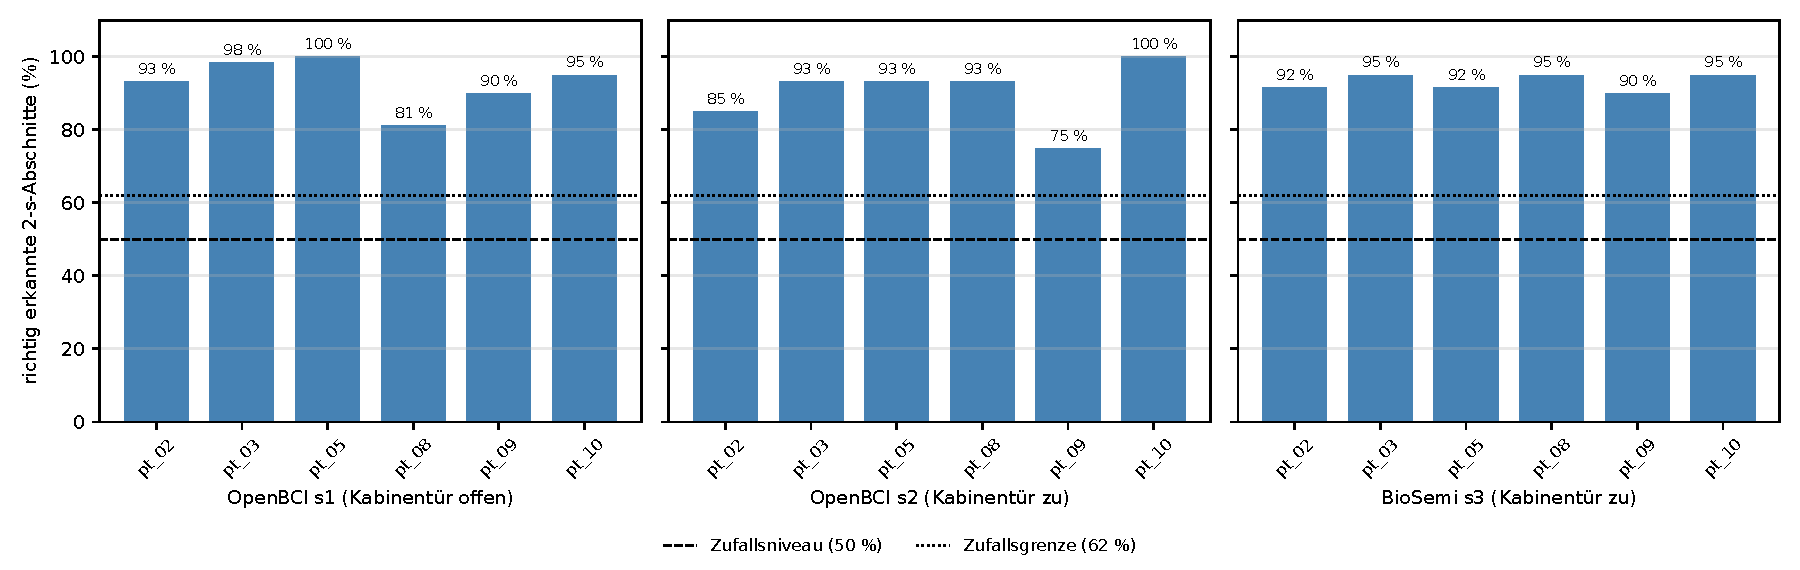
\includegraphics[width=0.9\textwidth]{diagramme/alpha_schalter_pro_person.pdf}
\quelle{Eigene Abbildung.}
\caption{Anteil der 2-Sekunden-Abschnitte, in denen allein anhand der Alpha-Power richtig erkannt wurde, ob die Augen geöffnet oder geschlossen waren, für jede der sechs Versuchspersonen in s1, s2 und s3 (links nach rechts); gestrichelt: Zufallsniveau 50\,\%, gepunktet: Zufallsgrenze 62\,\%}
\label{fig:alpha_schalter_pro_person}
\end{figure}

\section*{Zweite ergänzende Abbildungen zur Alpha-Auswertung}
\addcontentsline{toc}{section}{Zweite ergänzende Abbildungen zur Alpha-Auswertung}
\label{sec:erganzung2}
\begin{figure}[H]
\centering
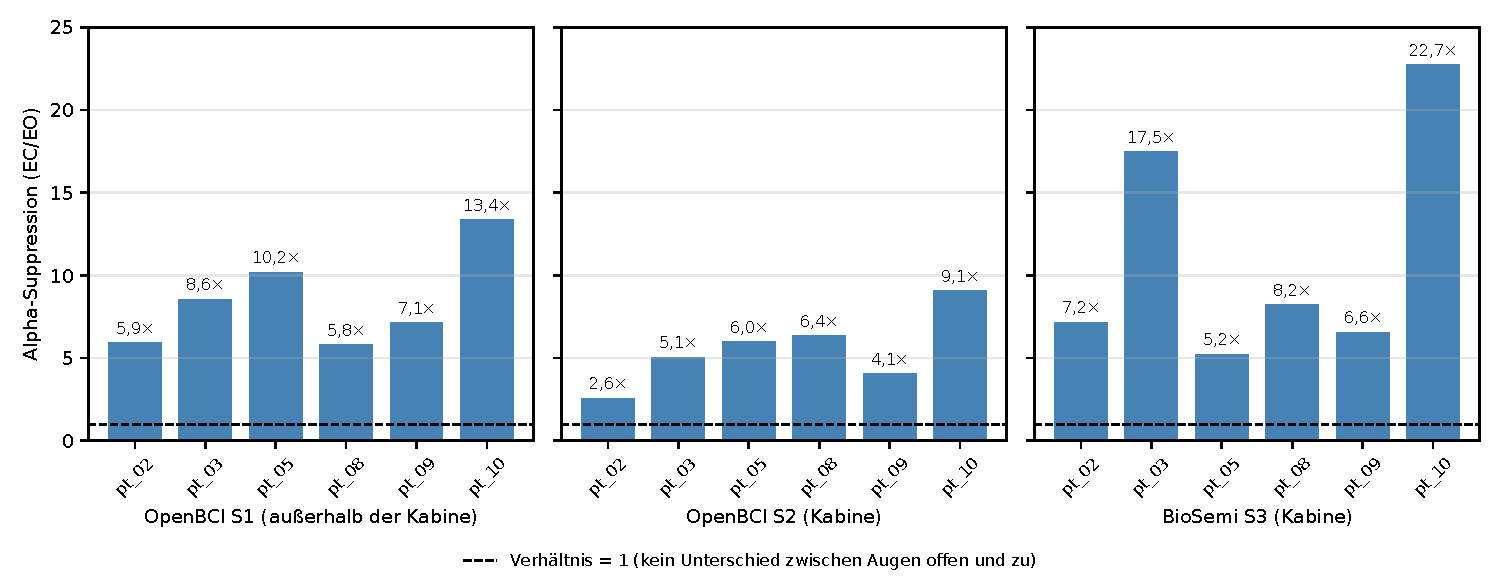
\includegraphics[width=0.9\textwidth]{diagramme/alpha_suppression_pro_person.pdf}
\quelle{Eigene Abbildung.}
\caption{Alpha-Suppression (Verhältnis der Alpha-Power bei geschlossenen zu geöffneten Augen, Elektroden O1/O2/P7/P8) für jede der sechs Versuchspersonen in s1, s2 und s3 (links nach rechts); Linie: Kriterium Verhältnis = 2}
\label{fig:alpha_suppression_pro_person}
\end{figure}



%Ein gemeinsames, alphabetisches Quellenverzeichnis ohne Unterteilung (CZG-Vorgabe)
\printbibliography[heading=bibintoc, title={Quellenverzeichnis}]


\begin{comment}%Verwendung siehe Präamble
\bibliography{literatur}
\bibliographystyle{dinat}

\bibliographyonline{literatur}
\bibliographystyleonline{dinat}
\end{comment}


	

\chapter*{Danksagung}
Wir danken Carolin Altmann und Christine Nussbaum für die fachliche Betreuung sowie die Bereitstellung der Geräte über das SchoolLab und das Institut für Psychologie. Sie unterstützten uns bei inhaltlichen Fragen und bei der Planung der Untersuchung.

Sophie Büttner und Vefa Arslan danken wir für die informatische Unterstützung und die Bereitstellung des Programmcodes zur Datenauswertung.

Bettina Kamchen und Kathrin Rauscher danken wir für die Unterstützung bei der Laborarbeit und der Betreuung der Probandinnen und Probanden.

Weiterhin danken wir Frau Meißner für die Betreuung als Fachbetreuerin an unserer Schule und die Hilfe bei der Lösung auftretender Probleme sowie Herrn Cebulski für die Betreuung als Seminarfachlehrer und seine Rückmeldungen zur Arbeit.

Abschließend danken wir allen Probandinnen und Probanden für ihre Teilnahme an der Untersuchung.

%Selbstständigkeitserklärung nach CZG-Dokumentenvorlage
\chapter*{Selbstständigkeitserklärung}
\addcontentsline{toc}{chapter}{Selbstständigkeitserklärung}
Wir erklären, dass wir die vorliegende Arbeit mit dem Titel \qt{Validierungsstudie eines portablen EEG-Gerätes von OpenBCI} selbstständig, ohne unzulässige fremde Hilfe angefertigt und nur unter Verwendung der angegebenen Literatur und Hilfsmittel verfasst haben. 
Sämtliche Stellen, die wörtlich oder inhaltlich anderen Werken entnommen sind, wurden unter Angabe der Quellen als Entlehnung kenntlich gemacht. 
Dies trifft besonders auch auf Quellen aus dem Internet zu. Gleichzeitig geben wir das Einverständnis, unsere Arbeit mittels einer Plagiatssoftware durch die Schule überprüfen zu lassen.

\vspace{0.3cm}
\noindent
Jena, den \makebox[4cm]{\hrulefill}

\vfill

\noindent\begin{tabular}{ll}
\makebox[2.5in]{\hrulefill} & \makebox[2.5in]{\hrulefill}\\
Katharina Ensslen& Alisa Fiedler\\[8ex]
\makebox[2.5in]{\hrulefill} & \makebox[2.5in]{\hrulefill}\\
Sophie Kleppe & Lorenz Kobylka\\
\end{tabular}

%Bei Drei Personen die Felder für Person Vier mit Leerzeichen ersetzen.


\end{document}
